\documentclass[11pt,oneside]{book}
\usepackage[utf8]{inputenc}
\usepackage[T1]{fontenc}
\usepackage{charter}
\usepackage{courier}
\usepackage[scaled=0.92]{helvet}
\usepackage{microtype}
\usepackage{geometry}
\geometry{
  letterpaper,
  left=1.1in,
  right=1.1in,
  top=1.0in,
  bottom=1.0in,
  headheight=24pt
}

\usepackage{amsmath,amssymb}
\usepackage{booktabs}
\usepackage{graphicx}
\usepackage{xcolor}
\usepackage{fancyhdr}
\usepackage{titlesec}
\usepackage{enumitem}
\usepackage{listings}
\usepackage{tcolorbox}
\tcbuselibrary{skins,breakable}
\usepackage{tikz}
\usetikzlibrary{arrows.meta,positioning,shapes.geometric,calc,decorations.pathreplacing,fit}

% Color Palette - Manning / O'Reilly inspired muted functional palette
\definecolor{textdark}{RGB}{30, 41, 59}       % Deep slate text
\definecolor{headingblue}{RGB}{15, 23, 42}    % Slate 900
\definecolor{codebg}{RGB}{248, 250, 252}       % Slate 50 background
\definecolor{codeframe}{RGB}{226, 232, 240}   % Slate 200 border
\definecolor{linkblue}{RGB}{2, 132, 199}      % Sky 600

% Callout colors
\definecolor{intuitionTeal}{RGB}{13, 148, 136}
\definecolor{intuitionBg}{RGB}{240, 253, 250}
\definecolor{hoodSlate}{RGB}{71, 85, 105}
\definecolor{hoodBg}{RGB}{248, 250, 252}
\definecolor{exampleBlue}{RGB}{37, 99, 235}
\definecolor{exampleBg}{RGB}{239, 246, 255}
\definecolor{mistakeAmber}{RGB}{217, 119, 6}
\definecolor{mistakeBg}{RGB}{254, 252, 232}
\definecolor{warningRed}{RGB}{220, 38, 38}
\definecolor{warningBg}{RGB}{254, 242, 242}
\definecolor{tryViolet}{RGB}{124, 58, 237}
\definecolor{tryBg}{RGB}{245, 243, 255}

% Typography & Spacing
\linespread{1.14}
\setlength{\parindent}{0pt}
\setlength{\parskip}{7pt plus 2pt minus 1pt}

% Section Titles Styling (Modern & Proportionate)
\titleformat{\chapter}[display]
  {\normalfont\sffamily\bfseries\color{headingblue}}
  {\vspace{-20pt}\flushleft\normalsize\scshape\color{gray}CHAPTER \thechapter}
  {6pt}
  {\huge\raggedright}[\vspace{10pt}\hrule height 0.8pt\vspace{14pt}]
\titlespacing*{\chapter}{0pt}{10pt}{20pt}

\titleformat{\section}
  {\normalfont\sffamily\Large\bfseries\color{headingblue}}
  {\thesection}{1em}{}
\titlespacing*{\section}{0pt}{16pt plus 3pt minus 2pt}{6pt}

\titleformat{\subsection}
  {\normalfont\sffamily\large\bfseries\color{headingblue}}
  {\thesubsection}{1em}{}
\titlespacing*{\subsection}{0pt}{12pt plus 2pt minus 2pt}{4pt}

\titleformat{\subsubsection}
  {\normalfont\sffamily\normalsize\bfseries\color{headingblue}}
  {\thesubsubsection}{1em}{}
\titlespacing*{\subsubsection}{0pt}{10pt plus 2pt minus 1pt}{3pt}

% Header & Footer
\pagestyle{fancy}
\fancyhf{}
\fancyhead[L]{\small\sffamily\color{gray}\nouppercase{\leftmark}}
\fancyhead[R]{\small\sffamily\bfseries\thepage}
\renewcommand{\headrulewidth}{0.4pt}
\renewcommand{\headrule}{\hbox to\headwidth{\color{gray!30}\leaders\hrule height \headrulewidth\hfill}}
\fancypagestyle{plain}{
  \fancyhf{}
  \fancyfoot[C]{\small\sffamily\thepage}
  \renewcommand{\headrulewidth}{0pt}
}

% Code Listings Styling
\lstset{
  backgroundcolor=\color{codebg},
  basicstyle=\ttfamily\footnotesize\color{textdark},
  breakatwhitespace=false,
  breaklines=true,
  captionpos=b,
  commentstyle=\color{gray!80!black}\itshape,
  frame=single,
  rulecolor=\color{codeframe},
  framerule=0.6pt,
  keepspaces=true,
  keywordstyle=\bfseries\color{blue!80!black},
  stringstyle=\color{green!50!black},
  numbers=left,
  numbersep=8pt,
  numberstyle=\tiny\color{gray!70},
  showspaces=false,
  showstringspaces=false,
  showtabs=false,
  tabsize=2,
  xleftmargin=12pt,
  framexleftmargin=10pt,
  framexrightmargin=4pt,
  framextopmargin=4pt,
  framexbottommargin=4pt
}

% 6 Pedagogical Callout Boxes (Muted, Left-Border Styling)
\newtcolorbox{intuitionbox}[1][]{
  enhanced,
  breakable,
  colback=intuitionBg,
  colframe=intuitionTeal,
  arc=1pt,
  boxrule=0pt,
  leftrule=3.5pt,
  top=6pt,bottom=6pt,left=10pt,right=10pt,
  coltitle=intuitionTeal,
  fonttitle=\sffamily\bfseries\small,
  title={Intuition \ifstrempty{#1}{}{: #1}},
  attach title to upper=\par\vspace{4pt}
}

\newtcolorbox{underthehoodbox}[1][]{
  enhanced,
  breakable,
  colback=hoodBg,
  colframe=hoodSlate,
  arc=1pt,
  boxrule=0pt,
  leftrule=3.5pt,
  top=6pt,bottom=6pt,left=10pt,right=10pt,
  coltitle=hoodSlate,
  fonttitle=\sffamily\bfseries\small,
  title={Under the Hood \ifstrempty{#1}{}{: #1}},
  attach title to upper=\par\vspace{4pt}
}

\newtcolorbox{realworldbox}[1][]{
  enhanced,
  breakable,
  colback=exampleBg,
  colframe=exampleBlue,
  arc=1pt,
  boxrule=0pt,
  leftrule=3.5pt,
  top=6pt,bottom=6pt,left=10pt,right=10pt,
  coltitle=exampleBlue,
  fonttitle=\sffamily\bfseries\small,
  title={Real-World Scenario \ifstrempty{#1}{}{: #1}},
  attach title to upper=\par\vspace{4pt}
}

\newtcolorbox{commonmistakebox}[1][]{
  enhanced,
  breakable,
  colback=mistakeBg,
  colframe=mistakeAmber,
  arc=1pt,
  boxrule=0pt,
  leftrule=3.5pt,
  top=6pt,bottom=6pt,left=10pt,right=10pt,
  coltitle=mistakeAmber,
  fonttitle=\sffamily\bfseries\small,
  title={Common Mistake \ifstrempty{#1}{}{: #1}},
  attach title to upper=\par\vspace{4pt}
}

\newtcolorbox{productionwarningbox}[1][]{
  enhanced,
  breakable,
  colback=warningBg,
  colframe=warningRed,
  arc=1pt,
  boxrule=0pt,
  leftrule=3.5pt,
  top=6pt,bottom=6pt,left=10pt,right=10pt,
  coltitle=warningRed,
  fonttitle=\sffamily\bfseries\small,
  title={Production Warning \ifstrempty{#1}{}{: #1}},
  attach title to upper=\par\vspace{4pt}
}

\newtcolorbox{tryityourselfbox}[1][]{
  enhanced,
  breakable,
  colback=tryBg,
  colframe=tryViolet,
  arc=1pt,
  boxrule=0pt,
  leftrule=3.5pt,
  top=6pt,bottom=6pt,left=10pt,right=10pt,
  coltitle=tryViolet,
  fonttitle=\sffamily\bfseries\small,
  title={Try It Yourself \ifstrempty{#1}{}{: #1}},
  attach title to upper=\par\vspace{4pt}
}

% Chapter Goals / Roadmaps Box
\newtcolorbox{chaptergoalsbox}{
  enhanced,
  breakable,
  colback=gray!4!white,
  colframe=gray!40!white,
  arc=2pt,
  boxrule=0.8pt,
  top=8pt,bottom=8pt,left=12pt,right=12pt,
  coltitle=headingblue,
  fonttitle=\sffamily\bfseries\small,
  title={Roadmap \& Prerequisites},
  attach title to upper=\par\vspace{4pt}
}

% Hyperref setup (Muted, readable links)
\usepackage[
  colorlinks=true,
  linkcolor=headingblue,
  citecolor=linkblue,
  urlcolor=linkblue,
  bookmarksnumbered=true,
  pdfstartview=FitH
]{hyperref}


\begin{document}
\frontmatter
\pagestyle{empty}

\begin{center}
  \vspace*{2cm}
  {\Huge\sffamily\bfseries\color{headingblue} Modern Engineering Curriculum}\\[12pt]
  {\Large\sffamily\color{gray} Volume II: AI Engineering}\\[8pt]
  {\large\sffamily\color{textdark} Vector Databases, Production RAG, Stateful Agents, Evaluations, and LLMOps}\\[30pt]
  \hrule height 1.2pt
  \vspace*{25pt}
  {\normalsize\sffamily A First-Principles Systems Textbook for Production AI Engineers}
\end{center}

\vspace{2.2cm}

\begin{tcolorbox}[
  enhanced,
  colback=white,
  colframe=gray!30!white,
  boxrule=0.8pt,
  arc=2pt,
  left=15pt,right=15pt,top=12pt,bottom=12pt
]
\sffamily\small
\textbf{About Volume II (AI Engineering):}
\begin{itemize}[leftmargin=15pt]
  \item \textbf{Who This Book Is For}: Software builders and engineers who have shipped applications---often with AI coding assistants---and want to master the math, storage engines, retrieval algorithms, state machines, and telemetry running underneath production AI systems.
  \item \textbf{Prerequisites}: Familiarity with reading basic Python functions, dictionaries, and lists, plus elementary comfort with SQL tables. Vector geometry, Transformer attention intuition, asynchronous \texttt{contextvars}, Pregel state machines, and OpenTelemetry tracing are all taught from first principles in the chapters where they appear.
  \item \textbf{Progression}: Volume II builds upward in dependency order: vector geometry and approximate indexes (Chapter~1), document parsing and contextual chunking (Chapter~2), hybrid sparse-dense retrieval and cross-encoder reranking (Chapter~3), tool-calling agent loops and safety boundaries (Chapter~4), durable LangGraph state machines (Chapter~5), semantic evaluation gates (Chapter~6), and OpenTelemetry observability, latency, and token economics (Chapter~7).
  \item \textbf{Curriculum Role}: Volume II bridges backend API and database engineering (Volume~I) with cloud security (Volume~III), distributed consensus systems (Volume~IV), and inference economics (Volume~V).
\end{itemize}
\end{tcolorbox}

\newpage
\pagestyle{fancy}
\tableofcontents
\newpage

\mainmatter

\chapter{Embeddings and Vector Databases: Geometry, Indexing, and Internals}
\label{chap:embeddings}

\begin{chaptergoalsbox}
\textbf{What You Will Learn:}
\begin{itemize}[leftmargin=15pt]
  \item Vector geometry from first principles: representing meaning as coordinates, dot products, cosine similarity, Euclidean ($L_2$) distance, and unit normalization.
  \item Why exact linear search hits a memory-bandwidth wall and why distances collapse in high dimensions (concentration of measure).
  \item Inverted File Indexes (IVF): Voronoi partitioning, $k$-means clustering, and $nlist/nprobe$ tuning.
  \item Hierarchical Navigable Small World (HNSW) graphs: building from 1D skip-lists to multi-layer proximity graphs.
  \item Out-of-core billion-scale search: Scalar Quantization (SQ8) vs Product Quantization (PQ), Vamana graphs, and Linux \texttt{io\_uring} in DiskANN.
  \item Storage engine internals: Qdrant's filtered segment traversal vs \texttt{pgvector}'s PostgreSQL buffer pool integration and distance operators.
\end{itemize}

\textbf{What You Should Already Understand:}
\begin{itemize}[leftmargin=15pt]
  \item Basic Python lists, loops, and functions.
  \item Elementary SQL (\texttt{SELECT}, \texttt{WHERE}, \texttt{ORDER BY}, \texttt{LIMIT}).
\end{itemize}

\textbf{Why This Topic Exists:}
Keyword search matches exact characters, so searching for \emph{``unauthorized SSH login''} misses a log entry reading \emph{``failed root password''}. Embedding models solve this by turning text into lists of numbers (vectors) where similar meanings land near each other. However, searching 10 million 1,536-dimensional vectors by brute force forces the CPU to stream 61.44 GB of data from RAM on every single query. Approximate Nearest Neighbor (ANN) indexes trade a tiny sliver of recall for millisecond latency.

\textbf{Motivating Practical Problem:}
A cybersecurity threat-intelligence platform ingests 50 million endpoint telemetry vectors per day. Analysts need sub-15 ms similarity search while filtering by \texttt{tenant\_id}, \texttt{operating\_system}, and \texttt{timestamp >= NOW() - INTERVAL '7 DAYS'}. A naive vector store either runs out of RAM or returns zero results when post-query filters discard all global nearest neighbors.
\end{chaptergoalsbox}

\section{From Meaning to Coordinates: 2D Vector Intuition}

Imagine you want a computer to recognize that two alerts describe the same incident even when they share zero words. Instead of storing only raw strings, an \textbf{embedding model} (a neural network trained on billions of text pairs) maps each piece of text to a list of floating-point numbers called a \textbf{vector}. Each coordinate captures a latent semantic feature.

To see how this works without drowning in 1,536 numbers, picture a tiny 2-dimensional world ($D = 2$) where axis 1 measures \emph{Security Risk} and axis 2 measures \emph{Routine Payroll/Finance}:
\begin{align*}
s_1 &= \text{``SSH brute force''}      &&\longrightarrow \vec{u} = (0.90,\; 0.10) \\
s_2 &= \text{``Failed root login''}    &&\longrightarrow \vec{v} = (0.85,\; 0.15) \\
s_3 &= \text{``Payroll CSV export''}   &&\longrightarrow \vec{w} = (0.10,\; 0.90)
\end{align*}
In this 2D plane, $\vec{u}$ and $\vec{v}$ point almost in the exact same direction (high security risk, low finance), while $\vec{w}$ points steeply upward toward finance.

\subsection{Three Ways to Measure Proximity}
Given any two vectors $\vec{u}, \vec{v} \in \mathbb{R}^D$, search engines rely on three fundamental formulas:

\begin{enumerate}[leftmargin=18pt]
  \item \textbf{Dot Product (Inner Product)}: Multiply matching coordinates and sum them up:
  \begin{equation}
  \langle \vec{u}, \vec{v} \rangle = \vec{u} \cdot \vec{v} = \sum_{i=1}^D u_i v_i
  \end{equation}
  For our tiny sentences:
  \[
  \vec{u} \cdot \vec{v} = (0.90)(0.85) + (0.10)(0.15) = 0.765 + 0.015 = 0.780
  \]
  \[
  \vec{u} \cdot \vec{w} = (0.90)(0.10) + (0.10)(0.90) = 0.090 + 0.090 = 0.180
  \]
  Here $0.780 > 0.180$, so $\vec{v}$ beats $\vec{w}$. However, notice a trap: suppose a verbose, off-topic finance report has the scaled vector $5\vec{w} = (0.50, 4.50)$. Its dot product with $\vec{u}$ is $(0.90)(0.50) + (0.10)(4.50) = 0.900 > 0.780$! Raw dot products reward \emph{longer} vectors (larger magnitudes), not just better alignment.

  \item \textbf{Cosine Similarity and Cosine Distance}: To ignore vector length and measure only the \textbf{angle} $\theta$ between two arrows, we divide each vector by its Euclidean length (its \textbf{$L_2$ norm}, $\|\vec{u}\|_2 = \sqrt{\sum_{i=1}^D u_i^2}$):
  \begin{equation}
  S_{\cos}(\vec{u}, \vec{v}) = \frac{\vec{u} \cdot \vec{v}}{\|\vec{u}\|_2 \|\vec{v}\|_2}, \qquad d_{\cos}(\vec{u}, \vec{v}) = 1 - S_{\cos}(\vec{u}, \vec{v})
  \end{equation}
  Computing lengths for our three sentences:
  \[
  \|\vec{u}\|_2 = \sqrt{0.90^2 + 0.10^2} \approx 0.9055, \quad
  \|\vec{v}\|_2 = \sqrt{0.85^2 + 0.15^2} \approx 0.8631, \quad
  \|\vec{w}\|_2 \approx 0.9055
  \]
  Therefore:
  \[
  S_{\cos}(\vec{u}, \vec{v}) = \frac{0.780}{0.9055 \times 0.8631} \approx 0.9980, \qquad
  S_{\cos}(\vec{u}, \vec{w}) = \frac{0.180}{0.9055 \times 0.9055} \approx 0.2195
  \]
  Even if we scale $\vec{w}$ to $5\vec{w} = (0.50, 4.50)$, its norm grows $5\times$ too, so $S_{\cos}(\vec{u}, 5\vec{w})$ stays $0.2195$. Cosine similarity is completely invariant to vector magnitude.

  \item \textbf{Euclidean Distance ($L_2$)}: Straight-line distance between vector tips:
  \begin{equation}
  d_{L_2}(\vec{u}, \vec{v}) = \|\vec{u} - \vec{v}\|_2 = \sqrt{\sum_{i=1}^D (u_i - v_i)^2}
  \end{equation}
  Between $\vec{u}$ and $\vec{v}$, $d_{L_2} = \sqrt{(0.05)^2 + (-0.05)^2} \approx 0.0707$, whereas between $\vec{u}$ and $\vec{w}$, $d_{L_2} = \sqrt{0.80^2 + (-0.80)^2} \approx 1.1314$.
\end{enumerate}

\begin{intuitionbox}[The Normalization Identity]
If you divide every vector by its own length once at ingestion time ($\|\vec{u}\|_2 = \|\vec{v}\|_2 = 1$), all vectors sit on the surface of a unit sphere, and all three metrics collapse into one:
\begin{equation}
\|\vec{u} - \vec{v}\|_2^2 = \|\vec{u}\|_2^2 + \|\vec{v}\|_2^2 - 2(\vec{u} \cdot \vec{v}) = 1 + 1 - 2\cos(\theta) = 2(1 - \cos(\theta)) = 2 \cdot d_{\cos}(\vec{u}, \vec{v})
\end{equation}
In production vector databases, \textbf{always pre-normalize vectors to unit length} (many models such as OpenAI's \texttt{text-embedding-3} already emit unit-normalized vectors). That eliminates square roots and divisions at query time, letting the CPU execute pure multiply-accumulate (SIMD) dot products.
\end{intuitionbox}

\section{Why Brute Force Fails at Scale: Bandwidth and High Dimensions}

\subsection{The Memory-Bandwidth Wall (Not Just FLOPs)}
Suppose your threat-intelligence platform stores $N = 10{,}000{,}000$ vectors with $D = 1536$ dimensions, each coordinate stored as a 32-bit float (`float32`, 4 bytes). Exact linear search (a \textbf{flat scan}) compares the query against every vector:
\begin{itemize}[leftmargin=18pt]
  \item \textbf{Floating-Point Arithmetic (Compute)}: Computing a dot product over $D = 1536$ dimensions performs 1,536 multiplications and 1,535 additions ($\approx 2D \approx 3{,}072$ FLOPs per vector, or $\approx 30.72\text{ billion FLOPs}$ across 10M vectors; squared $L_2$ adds subtraction for $3D \approx 46.08\text{ billion FLOPs}$). Modern server CPUs execute tens to hundreds of billions of FLOPs per second via AVX-512 SIMD lanes, so compute alone is rarely the bottleneck.
  \item \textbf{Memory Bandwidth (Data Movement)}: Each query must stream all $10^7 \times 1536 \times 4\text{ bytes} = 61{,}440{,}000{,}000\text{ bytes} \approx \mathbf{61.44\text{ GB}}$ of vector data from DRAM into CPU caches. On a server with 80 GB/s memory bandwidth, just reading the bytes off RAM takes $\approx 768\text{ ms}$ per query---making sub-15 ms latency physically impossible with a flat scan.
\end{itemize}

\subsection{The Curse of Dimensionality: Concentration of Measure}
Why can't we just use classic database trees (like B-Trees or $k$-d trees) to skip most of those 61.44 GB? Because spatial intuition from 2D and 3D breaks down completely in $\mathbb{R}^{1536}$.

Consider drawing two independent random vectors $\vec{u}, \vec{v}$ in $D$ dimensions. Each axis adds a small independent difference $(u_i - v_i)^2$. By the law of large numbers, summing 1,536 independent random terms averages out all lucky ``close'' or ``far'' extremes:
\begin{itemize}[leftmargin=18pt]
  \item For \textbf{unnormalized} standard normal vectors ($\vec{u}, \vec{v} \sim \mathcal{N}(0, I_D)$), $\mathbb{E}[\|\vec{u}-\vec{v}\|_2^2] = 2D$, so pairwise $L_2$ distances cluster tightly around $\sqrt{2D}$ (at $D=1536$, $\sqrt{3072} \approx 55.43$).
  \item For \textbf{unit-normalized} vectors ($\|\vec{u}\|_2 = \|\vec{v}\|_2 = 1$), random pairs become nearly perpendicular ($\vec{u} \cdot \vec{v} \to 0$), so by the Normalization Identity their $L_2$ distances concentrate tightly around $\sqrt{2} \approx 1.414$!
\end{itemize}

\begin{figure}[htbp]
\centering
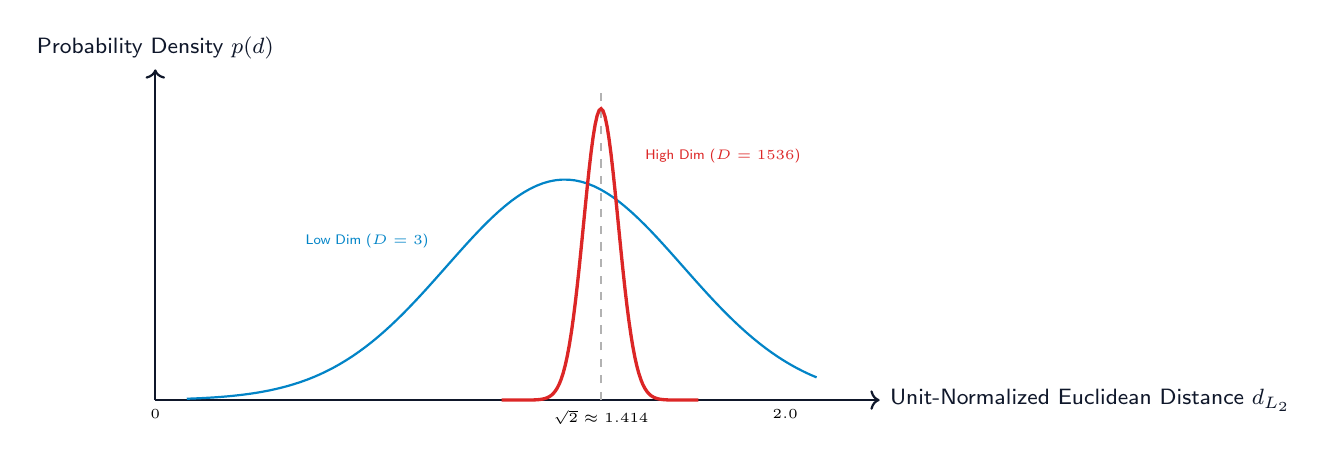
\begin{tikzpicture}
\draw[->, thick, color=headingblue] (0,0) -- (9.2,0) node[right, font=\sffamily\footnotesize] {Unit-Normalized Euclidean Distance $d_{L_2}$};
\draw[->, thick, color=headingblue] (0,0) -- (0,4.2) node[above, font=\sffamily\footnotesize] {Probability Density $p(d)$};

% Reference tick at sqrt(2) ~ 1.414 -> map d in [0, 2.2] to x in [0, 8.8] (scale 4.0)
% sqrt(2) * 4 = 5.656
\draw[dashed, color=gray!60] (5.66, 0) -- (5.66, 3.9);
\node[below, font=\tiny\sffamily] at (5.66, 0) {$\sqrt{2} \approx 1.414$};
\node[below, font=\tiny\sffamily] at (0, 0) {$0$};
\node[below, font=\tiny\sffamily] at (8.0, 0) {$2.0$};

% Low-D (D=3) Wide
\draw[thick, color=linkblue, domain=0.4:8.4, samples=100]
  plot (\x, {2.8 * exp(-0.5 * ((\x - 5.2)/1.5)^2)})
  node[above left, font=\tiny\sffamily, color=linkblue] at (3.6, 1.8) {Low Dim ($D=3$)};

% High-D (D=1536) Sharp spike at sqrt(2)
\draw[very thick, color=warningRed, domain=4.4:6.9, samples=100]
  plot (\x, {3.7 * exp(-0.5 * ((\x - 5.66)/0.22)^2)});
\node[right, font=\tiny\sffamily, color=warningRed] at (6.1, 3.1) {High Dim ($D=1536$)};

\end{tikzpicture}
\caption{Concentration of Measure for Unit-Normalized Vectors: As $D$ increases from $3$ to $1536$, random vectors become mutually orthogonal and pairwise $L_2$ distances collapse into a narrow spike around $\sqrt{2} \approx 1.414$ (unnormalized $\mathcal{N}(0, I_D)$ vectors likewise collapse around $\sqrt{2D}$).}
\label{fig:v2-ch01-concentration}
\end{figure}

In high dimensions, the gap between the nearest neighbor $d_{\min}$ and farthest neighbor $d_{\max}$ shrinks relative to $d_{\min}$:
\begin{equation}
\lim_{D \to \infty} \frac{d_{\max} - d_{\min}}{d_{\min}} = 0
\end{equation}
Space-partitioning trees ($k$-d trees, $R$-trees) must inspect almost every branch box because every box overlaps the query sphere, collapsing back to $O(N)$ linear scans. To search in milliseconds, we turn to \textbf{clustering (IVF)}, \textbf{proximity graphs (HNSW)}, and \textbf{compression (PQ)}.

\section{The Inverted File Index (IVF): Neighborhoods via Voronoi Cells}

Think of how a delivery network avoids scanning every house in a country: it groups houses into postal ZIP codes, puts a post office (a \textbf{centroid}) in the center of each zone, and only visits the 1 or 2 ZIP codes closest to the destination.

In vector search, this partitioning is called a \textbf{Voronoi diagram} (Figure~\ref{fig:v2-ch01-ivf}). Given $nlist$ centroids $\{\vec{c}_1, \dots, \vec{c}_{nlist}\}$, every point in space belongs to whichever centroid is closest. Each centroid owns an \textbf{inverted list} holding only the vectors inside its cell.

\begin{figure}[htbp]
\centering
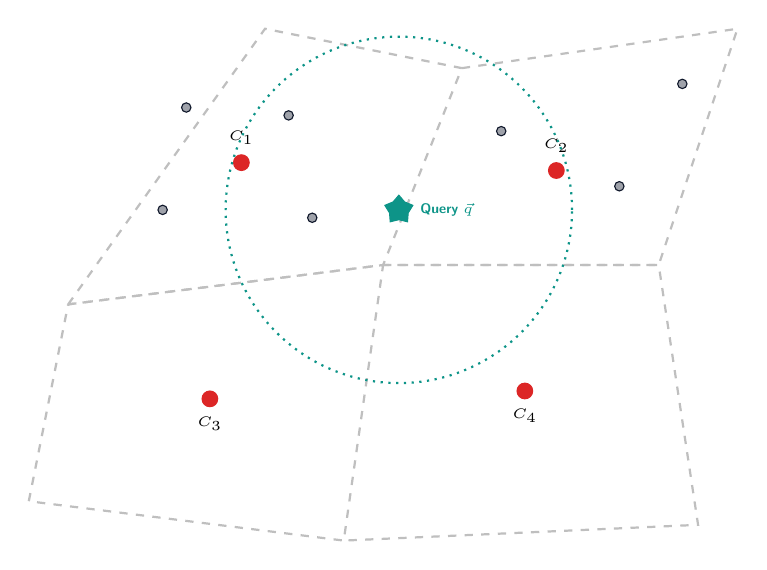
\begin{tikzpicture}[
  centroid/.style={draw=warningRed, fill=warningRed, circle, inner sep=2pt},
  point/.style={draw=headingblue, fill=headingblue!40, circle, inner sep=1.2pt},
  cell/.style={draw=gray!50, dashed, thick}
]

\draw[cell] (0,0) -- (2.5, 3.5) -- (5, 3.0) -- (4, 0.5) -- cycle;
\draw[cell] (5, 3.0) -- (8.5, 3.5) -- (7.5, 0.5) -- (4, 0.5);
\draw[cell] (0,0) -- (4, 0.5) -- (3.5, -3.0) -- (-0.5, -2.5) -- cycle;
\draw[cell] (4, 0.5) -- (7.5, 0.5) -- (8.0, -2.8) -- (3.5, -3.0);

\node[centroid, label={[font=\tiny\sffamily]above:$C_1$}] (c1) at (2.2, 1.8) {};
\node[centroid, label={[font=\tiny\sffamily]above:$C_2$}] (c2) at (6.2, 1.7) {};
\node[centroid, label={[font=\tiny\sffamily]below:$C_3$}] (c3) at (1.8, -1.2) {};
\node[centroid, label={[font=\tiny\sffamily]below:$C_4$}] (c4) at (5.8, -1.1) {};

\node[point] at (1.2, 1.2) {}; \node[point] at (2.8, 2.4) {}; \node[point] at (1.5, 2.5) {};
\node[point] at (3.1, 1.1) {};
\node[point] at (5.5, 2.2) {}; \node[point] at (7.0, 1.5) {}; \node[point] at (7.8, 2.8) {};

\node[draw=intuitionTeal, fill=intuitionTeal, star, star points=5, inner sep=2.5pt, label={[font=\tiny\sffamily\bfseries, color=intuitionTeal]right:Query $\vec{q}$}] (q) at (4.2, 1.2) {};
\draw[draw=intuitionTeal, thick, dotted] (q) circle (2.2cm);

\end{tikzpicture}
\caption{IVF Voronoi Partitioning: Query $\vec{q}$ sits near the boundary between cells $C_1$ and $C_2$. Setting $nprobe=2$ checks both neighboring cells so boundary points are not missed.}
\label{fig:v2-ch01-ivf}
\end{figure}

\subsection{How $k$-Means Learns the Centroids}
How do we pick good centroids? We run \textbf{$k$-means clustering}:
\begin{enumerate}[leftmargin=18pt]
  \item Pick $nlist$ sample vectors as initial centroids.
  \item \textbf{Assignment step}: Assign every training vector to its nearest centroid.
  \item \textbf{Update step}: Recompute each centroid as the coordinate-wise arithmetic mean of all vectors assigned to it.
  \item Repeat Steps 2--3 until assignments stop changing (or reach \texttt{max\_iters}).
\end{enumerate}

Listing~\ref{lst:v2-ch01-ivf} implements a complete IVF index with real $k$-means iterations.

\begin{lstlisting}[language=Python, label={lst:v2-ch01-ivf}, caption={Minimal Inverted File Index (IVF) with Iterative $k$-Means}]
import numpy as np

class MinimalIVFIndex:
    def __init__(self, nlist: int = 100, nprobe: int = 5):
        self.nlist = nlist
        self.nprobe = nprobe
        self.centroids: np.ndarray | None = None
        self.inverted_lists: dict[int, list[tuple[int, np.ndarray]]] = {}

    def train_and_index(
        self, vectors: np.ndarray, max_iters: int = 15, seed: int = 42
    ) -> None:
        rng = np.random.default_rng(seed)
        N, _ = vectors.shape
        init_idx = rng.choice(N, self.nlist, replace=False)
        self.centroids = vectors[init_idx].astype(np.float64).copy()

        assignments = np.zeros(N, dtype=int)
        for it in range(max_iters):
            # Broadcast shape (N, 1, D) - (1, nlist, D) -> (N, nlist) distances
            dists = np.linalg.norm(
                vectors[:, None, :] - self.centroids[None, :, :], axis=2
            )
            new_assignments = np.argmin(dists, axis=1)
            if it > 0 and np.array_equal(new_assignments, assignments):
                break
            assignments = new_assignments

            # Update each centroid to the mean of its assigned members
            for c_idx in range(self.nlist):
                members = vectors[assignments == c_idx]
                if len(members) > 0:
                    self.centroids[c_idx] = members.mean(axis=0)

        self.inverted_lists = {i: [] for i in range(self.nlist)}
        for vec_id, (vec, c_idx) in enumerate(zip(vectors, assignments)):
            self.inverted_lists[int(c_idx)].append((vec_id, vec))

    def search(self, query: np.ndarray, k: int = 5) -> list[tuple[int, float]]:
        assert self.centroids is not None
        centroid_dists = np.linalg.norm(self.centroids - query, axis=1)
        probed_centroids = np.argsort(centroid_dists)[:self.nprobe]

        candidates: list[tuple[int, float]] = []
        for c_idx in probed_centroids:
            for vec_id, vec in self.inverted_lists[int(c_idx)]:
                dist = float(np.linalg.norm(vec - query))
                candidates.append((vec_id, dist))

        candidates.sort(key=lambda x: x[1])
        return candidates[:k]
\end{lstlisting}

\textbf{Step-by-Step Code Walkthrough:} Suppose we index six 2D vectors with \texttt{nlist=2, nprobe=1}: three near $(0.15, 0.18)$ (IDs $0, 1, 2$) and three near $(0.85, 0.85)$ (IDs $3, 4, 5$).
\begin{enumerate}[leftmargin=18pt]
  \item Lines 15--16 randomly pick two starting centroids (say vector 0 and vector 1, both in the lower cluster!).
  \item In iteration 0 (lines 21--24), distances place vector 0 into cluster 0 and vectors $1..5$ into cluster 1.
  \item Lines 30--33 recompute the centroids: cluster 1's centroid jumps toward the average of vectors $1..5$, pulling it up toward $(0.7, 0.7)$. By iteration 2, cluster 0 captures IDs $\{0, 1, 2\}$ with centroid $\approx (0.15, 0.18)$ and cluster 1 captures IDs $\{3, 4, 5\}$ with centroid $\approx (0.85, 0.85)$, and the loop stops early at line 26.
  \item When \texttt{search(query=[0.88, 0.82], k=2)} runs (lines 39--50), it measures distance to just 2 centroids, picks cluster 1, and scans only 3 vectors instead of 6.
\end{enumerate}

\begin{commonmistakebox}[Setting $nprobe=1$ on Boundary Queries]
As shown in Figure~\ref{fig:v2-ch01-ivf}, a query sitting near the edge between Voronoi cells $C_1$ and $C_2$ may have its true nearest neighbor just across the border in $C_2$. If $nprobe=1$, recall often stalls around 65--75\%. Raising $nlist \approx 4\sqrt{N}$ and probing $nprobe \in [16, 64]$ cells recovers $>95\%$ recall while still skipping $>98\%$ of the dataset.
\end{commonmistakebox}

\section{HNSW Graphs: From 1D Skip-Lists to Multi-Layer Navigation}

To understand \textbf{Hierarchical Navigable Small World (HNSW)} graphs (Malkov \& Yashunin, 2020), start with a 1-dimensional sorted linked list of 1,000 numbers. Walking one node at a time from index 0 to 842 takes 842 hops ($O(N)$). A \textbf{skip-list} fixes this by adding express lanes above the base list:
\begin{itemize}[leftmargin=18pt]
  \item \textbf{Layer 2 (Express Highway)}: Only $\sim 1\%$ of nodes appear here, linked by huge jumps ($0 \to 400 \to 800$).
  \item \textbf{Layer 1 (Regional Road)}: $\sim 10\%$ of nodes appear here, taking medium steps ($800 \to 830 \to 840$).
  \item \textbf{Layer 0 (Local Street)}: Every single node lives here ($840 \to 841 \to 842$).
\end{itemize}
Search takes $O(\log N)$ hops because you cover huge distances at the top and only inspect fine neighbors at the bottom.

HNSW applies the exact same multi-layer expressway idea to vectors in $\mathbb{R}^D$ (Figure~\ref{fig:v2-ch01-hnsw}). Because vectors have no 1D left-to-right order, edges connect each node to nearby vectors (plus carefully pruned long-range bridges for navigability).

\begin{figure}[htbp]
\centering
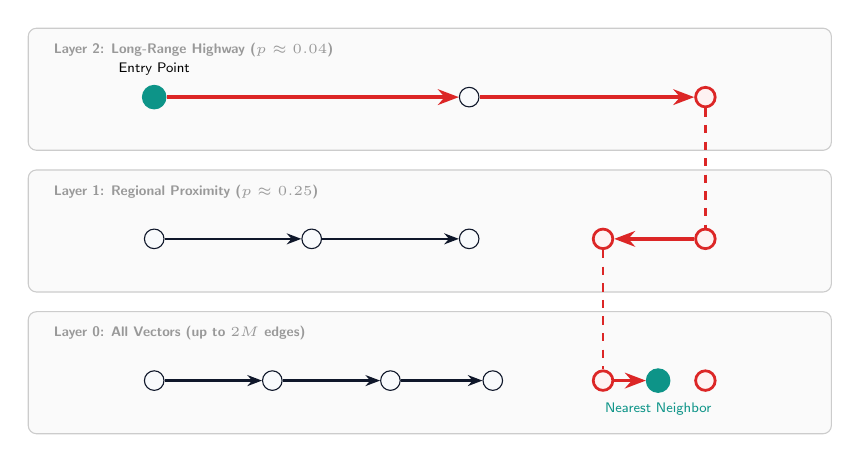
\begin{tikzpicture}[
  node/.style={circle, draw=headingblue, fill=codebg, inner sep=2.5pt},
  activenode/.style={circle, draw=warningRed, fill=warningBg, inner sep=2.5pt, line width=1pt},
  entrynode/.style={circle, draw=intuitionTeal, fill=intuitionTeal, inner sep=3pt},
  layer/.style={draw=gray!40, fill=gray!4, rounded corners=3pt, minimum width=10.2cm, minimum height=1.55cm},
  arrow/.style={-{Stealth[scale=0.8]}, thick, color=headingblue},
  route/.style={-{Stealth[scale=0.9]}, very thick, color=warningRed}
]

\node[layer] (l2) at (0, 3.6) {};
\node[anchor=west, font=\sffamily\bfseries\tiny, color=gray!80] at (-4.9, 4.1) {Layer 2: Long-Range Highway ($p \approx 0.04$)};
\node[entrynode, label={[font=\tiny\sffamily]above:Entry Point}] (e2) at (-3.5, 3.5) {};
\node[node] (n21) at (0.5, 3.5) {};
\node[activenode] (n22) at (3.5, 3.5) {};
\draw[route] (e2) -- (n21);
\draw[route] (n21) -- (n22);

\node[layer] (l1) at (0, 1.8) {};
\node[anchor=west, font=\sffamily\bfseries\tiny, color=gray!80] at (-4.9, 2.3) {Layer 1: Regional Proximity ($p \approx 0.25$)};
\node[node] (n11) at (-3.5, 1.7) {};
\node[node] (n12) at (-1.5, 1.7) {};
\node[node] (n13) at (0.5, 1.7) {};
\node[activenode] (n14) at (2.2, 1.7) {};
\node[activenode] (n15) at (3.5, 1.7) {};
\draw[arrow] (n11) -- (n12); \draw[arrow] (n12) -- (n13);
\draw[route] (n15) -- (n14);

\node[layer] (l0) at (0, 0) {};
\node[anchor=west, font=\sffamily\bfseries\tiny, color=gray!80] at (-4.9, 0.5) {Layer 0: All Vectors (up to $2M$ edges)};
\node[node] (n01) at (-3.5, -0.1) {};
\node[node] (n02) at (-2.0, -0.1) {};
\node[node] (n03) at (-0.5, -0.1) {};
\node[node] (n04) at (0.8, -0.1) {};
\node[activenode] (n05) at (2.2, -0.1) {};
\node[activenode] (n06) at (3.5, -0.1) {};
\node[entrynode, label={[font=\tiny\sffamily, color=intuitionTeal]below:Nearest Neighbor}] (target) at (2.9, -0.1) {};
\draw[arrow] (n01) -- (n02); \draw[arrow] (n02) -- (n03); \draw[arrow] (n03) -- (n04);
\draw[route] (n05) -- (target);

\draw[dashed, color=warningRed, thick] (n22) -- (n15);
\draw[dashed, color=warningRed, thick] (n14) -- (n05);

\end{tikzpicture}
\caption{HNSW Multi-Layer Graph Traversal: Greedy search crosses long-range edges on sparse upper layers, then drops vertically when no neighbor is closer to the query.}
\label{fig:v2-ch01-hnsw}
\end{figure}

\subsection{Probabilistic Layer Assignment and Key Hyperparameters}
When inserting a new vector, its highest layer $l$ is sampled from an exponentially decaying distribution:
\begin{equation}
l = \lfloor -\ln(\text{uniform}(0, 1)) \cdot m_L \rfloor, \qquad m_L = \frac{1}{\ln(M)}
\end{equation}
For example, if $M = 16$, then $m_L \approx 0.361$. A random number $u \in (0, 1)$ reaches layer $1$ or higher only when $-\ln(u)/\ln(16) \ge 1$, i.e., $u \le 1/16 = 6.25\%$, and reaches layer $2$ or higher with probability $(1/16)^2 \approx 0.39\%$. Layer 0 holds all $N$ vectors.

Three knobs govern HNSW behavior:
\begin{itemize}[leftmargin=18pt]
  \item \textbf{$M$} (typically $16 \le M \le 64$): Maximum edges per node on upper layers ($2M$ on Layer 0). Larger $M$ prevents dead-end traps in clustered data at the cost of RAM.
  \item \textbf{$efConstruction$} (typically $100 \le efConstruction \le 400$): Size of the dynamic candidate queue explored when wiring a newly inserted vector. Higher values build a cleaner graph but slow down ingestion.
  \item \textbf{$efSearch$} (typically $32 \le efSearch \le 256$): Candidate queue size at query time. You can tune this per request without rebuilding the index.
\end{itemize}

\section{DiskANN: Quantization (SQ8 vs PQ) and NVMe Search}

HNSW's drawback is RAM cost. Storing 1 billion 768-dimensional `float32` vectors with $M=32$ edges requires:
\begin{equation}
10^9 \times \bigl(768 \times 4\text{ bytes} + \text{edge pointers}\bigr) > 3.3\text{ TB of RAM}
\end{equation}
\textbf{DiskANN} (Subramanya et al., 2019) keeps a compressed guide in RAM while storing full vectors and adjacency lists on NVMe SSDs. To understand how DiskANN shrinks 3.3 TB down to tens of gigabytes, we must distinguish two compression schemes:

\begin{enumerate}[leftmargin=18pt]
  \item \textbf{Scalar Quantization (SQ8 --- 1 byte per dimension)}: Each individual 32-bit float ($4$ bytes) is linearly scaled into an 8-bit integer ($0\dots 255$, $1$ byte). A 768-dimensional vector shrinks by $4\times$, from $3{,}072$ bytes to $768$ bytes.
  \item \textbf{Product Quantization (PQ --- subvector codebooks)}: Rather than keeping 1 byte per dimension, PQ splits a $D$-dimensional vector into $M_{\text{pq}}$ smaller \emph{subvectors} (for instance, $D = 768$ split into $M_{\text{pq}} = 64$ chunks of $12$ dimensions each). Inside each 12-dimensional subspace, $k$-means learns $256$ representative centroids (a 1-byte ID, $0\dots 255$). Each 12-float chunk is replaced by a single 1-byte codebook ID! The entire 768-dimensional vector shrinks from $3{,}072$ bytes down to just \textbf{64 bytes} ($48\times$ compression).
\end{enumerate}

\begin{figure}[htbp]
\centering
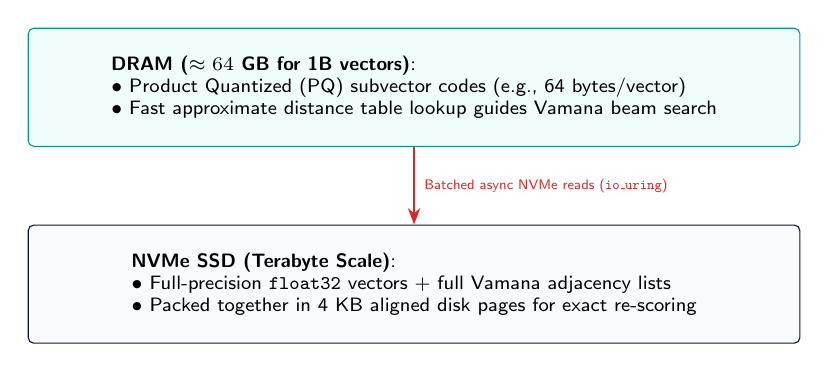
\begin{tikzpicture}[
  ram/.style={draw=intuitionTeal, fill=intuitionBg, rounded corners=2pt, font=\sffamily\scriptsize, minimum width=9.8cm, minimum height=1.5cm, align=left},
  ssd/.style={draw=headingblue, fill=codebg, rounded corners=2pt, font=\sffamily\scriptsize, minimum width=9.8cm, minimum height=1.5cm, align=left},
  arrow/.style={-{Stealth[scale=0.9]}, thick, color=warningRed}
]

\node[ram] (r) at (0, 2.0) {
  \textbf{DRAM ($\approx 64$ GB for 1B vectors)}:\\
  $\bullet$ Product Quantized (PQ) subvector codes (e.g., 64 bytes/vector)\\
  $\bullet$ Fast approximate distance table lookup guides Vamana beam search
};

\node[ssd] (s) at (0, -0.5) {
  \textbf{NVMe SSD (Terabyte Scale)}:\\
  $\bullet$ Full-precision \texttt{float32} vectors + full Vamana adjacency lists\\
  $\bullet$ Packed together in 4 KB aligned disk pages for exact re-scoring
};

\draw[arrow] (r.south) -- (s.north) node[midway, right, font=\tiny\sffamily, color=warningRed] {Batched async NVMe reads (\texttt{io\_uring})};

\end{tikzpicture}
\caption{DiskANN Architecture: Compact PQ subvector codes in DRAM steer the search; batched NVMe reads fetch full-precision vectors and neighbors for final re-scoring.}
\label{fig:v2-ch01-diskann}
\end{figure}

\begin{underthehoodbox}[Vamana Graphs and Linux \texttt{io\_uring}]
DiskANN combines PQ with two systems innovations (Figure~\ref{fig:v2-ch01-diskann}):
\begin{enumerate}
  \item \textbf{Vamana Single-Layer Graph}: Instead of HNSW's multi-layer hierarchy (which causes extra disk hops per layer), Vamana builds one flat graph with $\alpha$-pruned long-range edges ($\alpha \ge 1.2$), reaching targets in fewer SSD round-trips.
  \item \textbf{Linux \texttt{io\_uring}}: Traditional file reads block a thread per I/O syscall. \texttt{io\_uring} is a Linux kernel interface built on shared memory ring buffers between user space and the kernel: the search engine submits a batch of 16 or 32 NVMe page reads in a single syscall and harvests completions asynchronously, saturating NVMe queue depth in single-digit milliseconds.
\end{enumerate}
\end{underthehoodbox}

\section{Engine Internals: Qdrant vs \texttt{pgvector}}

\subsection{Qdrant: Segments and Filtered HNSW}
Qdrant (written in Rust) splits collections into immutable \textbf{segments}, building an HNSW index per segment in background workers. Its standout feature is how it handles metadata filters (like \texttt{WHERE tenant\_id = 42}):
\begin{itemize}[leftmargin=18pt]
  \item \textbf{Pre-filtering} filters rows first, then searches—which either falls back to a brute-force scan or breaks an HNSW graph into disconnected islands.
  \item \textbf{Post-filtering} finds the top-$k$ global vectors first and discards non-matching rows—causing catastrophic zero-result failures on selective filters.
  \item \textbf{Filtered HNSW (Qdrant)}: Checks a fast payload bitset \emph{during} graph traversal, continuing to hop through matching edges (plus fallback links) until $k$ valid matches are collected.
\end{itemize}

\subsection{\texttt{pgvector}: PostgreSQL Pages, Buffer Pools, and Operators}
PostgreSQL stores table rows and index nodes inside 8 KB disk pages cached in RAM inside a shared memory region called \texttt{shared\_buffers} (backed by the OS page cache). \texttt{pgvector} implements HNSW directly as a PostgreSQL index access method, giving you ACID transactions and relational joins in one database.

PostgreSQL exposes three distance operators for \texttt{vector} columns (remember: \texttt{ORDER BY} sorts ascending, smallest first):
\begin{itemize}[leftmargin=18pt]
  \item \texttt{<->} (\texttt{vector\_l2\_ops}): Euclidean $L_2$ distance $\|\vec{u} - \vec{v}\|_2$.
  \item \texttt{<=>} (\texttt{vector\_cosine\_ops}): Cosine distance $1 - \cos(\theta)$.
  \item \texttt{<\#>} (\texttt{vector\_ip\_ops}): \emph{Negative} inner product $-\langle \vec{u}, \vec{v} \rangle$ (negated so the largest dot product becomes the smallest number for \texttt{ORDER BY ... ASC}).
\end{itemize}
Your query's \texttt{ORDER BY} operator \textbf{must match} the operator class specified in \texttt{CREATE INDEX}, or PostgreSQL ignores the index and runs a sequential table scan.

\begin{lstlisting}[language=SQL, label={lst:v2-ch01-pgvector}, caption={pgvector Production Schema, Index Creation, and Filtered Query}]
CREATE EXTENSION IF NOT EXISTS vector;

CREATE TABLE threat_signatures (
    id UUID PRIMARY KEY DEFAULT gen_random_uuid(),
    tenant_id INT NOT NULL,
    observed_at TIMESTAMPTZ NOT NULL,
    embedding vector(1536) NOT NULL
);

-- Operator class vector_cosine_ops requires <=> in ORDER BY
CREATE INDEX idx_threat_hnsw ON threat_signatures
USING hnsw (embedding vector_cosine_ops)
WITH (m = 24, ef_construction = 128);

SET hnsw.ef_search = 64;

EXPLAIN (ANALYZE, BUFFERS)
SELECT id, tenant_id, 1 - (embedding <=> '[0.012, -0.045, ...]'::vector) AS similarity
FROM threat_signatures
WHERE tenant_id = 42 AND observed_at >= NOW() - INTERVAL '7 days'
ORDER BY embedding <=> '[0.012, -0.045, ...]'::vector
LIMIT 10;
\end{lstlisting}

\begin{productionwarningbox}[\texttt{pgvector} Shared Buffer Thrashing]
An HNSW index over 1,000,000 vectors of $D = 1536$ exceeds 6 GB on disk. If PostgreSQL \texttt{shared\_buffers} is left at 128 MB and host RAM is small, every random HNSW graph hop misses cache and reads an 8 KB page from disk, driving latency from 5 ms to 800+ ms. Size host RAM and \texttt{shared\_buffers} (typically 25--40\% of RAM, leaving room for the OS page cache) so the active HNSW graph stays memory-resident.
\end{productionwarningbox}

\begin{realworldbox}[Diagnosing Zero-Result Post-Filtering and Seq Scan Fallbacks]
A multi-tenant healthcare search API began returning empty lists for smaller clinics while larger hospitals saw normal results. Inspecting the query trace and PostgreSQL execution plan revealed two issues:
\begin{lstlisting}[basicstyle=\ttfamily\scriptsize]
INFO  query="chest pain triage" hospital_id="H-901" raw_ann_hits=10 post_filter_hits=0
EXPLAIN ANALYZE:
Limit  (actual time=412.18..412.18 rows=0 loops=1)
  -> Seq Scan on clinical_notes (actual time=412.15..412.15 rows=0)
       Filter: (hospital_id = 'H-901')
\end{lstlisting}
\textbf{Root Causes \& Fix}: First, Hospital \texttt{H-901} held only 0.2\% of total rows, so taking the global top 10 vectors and filtering afterward discarded every hit. Second, a separate query used \texttt{<->} against an index created with \texttt{vector\_cosine\_ops} (\texttt{<=>}), forcing a 412 ms sequential scan. Switching to Qdrant's payload-indexed traversal (or \texttt{pgvector} 0.8+ iterative index scans with matching \texttt{<=>} operators and a B-tree index on \texttt{hospital\_id}) eliminated empty responses and restored 8 ms $p95$ latency.
\end{realworldbox}

\begin{tryityourselfbox}[Benchmarking Exact Scan vs Cosine Normalization in Pure Python]
Write a short Python script using \texttt{random.Random(42)} (no external libraries needed) to:
\begin{enumerate}
  \item Generate 5,000 random unit-normalized vectors of dimension $D = 64$.
  \item Generate a unit-normalized query vector $\vec{q}$.
  \item Verify numerically that sorting by Euclidean distance $\|\vec{q} - \vec{v}\|_2^2$ yields the \emph{exact same} top-5 IDs as sorting by $2(1 - \langle \vec{q}, \vec{v} \rangle)$.
  \item Measure the elapsed milliseconds for a flat scan over 5,000 vectors and extrapolate to 10,000,000 vectors.
\end{enumerate}
(Worked solution is provided in Section~1.8.)
\end{tryityourselfbox}

\section{Chapter Summary \protect\& Key Takeaways}
\begin{itemize}[leftmargin=18pt]
  \item \textbf{Normalization Identity}: For unit-length vectors ($\|\vec{v}\|_2 = 1$), Euclidean distance squared, Cosine distance, and negative Inner Product produce identical rankings.
  \item \textbf{Bandwidth \& High Dimensions}: Brute-force search over 10M 1536-dim \texttt{float32} vectors streams 61.44 GB of RAM per query, while concentration of measure collapses distance variance around $\sqrt{2}$ (unit-normalized) or $\sqrt{2D}$ (unnormalized normal).
  \item \textbf{IVF}: Partitions vectors into Voronoi cells via $k$-means; tune $nlist$ and $nprobe$ to balance speed against boundary recall loss.
  \item \textbf{HNSW}: Extends 1D skip-lists to metric spaces, achieving $O(\log N \cdot D)$ query complexity governed by $M$, $efConstruction$, and $efSearch$.
  \item \textbf{Quantization \& DiskANN}: SQ8 compresses floats to 1 byte/dim ($4\times$), whereas Product Quantization encodes subvectors as 1-byte codebook IDs ($32\times$--$64\times$) so Vamana graphs can traverse DRAM guides and batch NVMe reads via \texttt{io\_uring}.
  \item \textbf{Engine Selection}: Match operators (\texttt{<=>}, \texttt{<->}, \texttt{<\#>}) to index opclasses in \texttt{pgvector}, and prefer in-traversal filtering over post-filtering for selective multi-tenant queries.
\end{itemize}

\section{Exercises}

\subsection*{Mechanics}
\textbf{Exercise \thechapter.1}: Prove algebraically that for any two unit vectors $\vec{u}, \vec{v} \in \mathbb{R}^D$ ($\|\vec{u}\|_2 = \|\vec{v}\|_2 = 1$), $\|\vec{u} - \vec{v}\|_2^2 = 2 - 2\langle \vec{u}, \vec{v} \rangle$.

\textbf{Exercise \thechapter.2}: Calculate the RAM (in GB, base 10) required for an unquantized HNSW index of $10{,}000{,}000$ vectors with $D = 1536$ (\texttt{float32}), assuming $M = 32$ bidirectional edges on Layer 0 with 8-byte integer pointers and 10\% upper-layer overhead. Then calculate the vector payload size if compressed using Product Quantization with $M_{\text{pq}} = 96$ subvectors (1 byte/subvector).

\subsection*{Debugging}
\textbf{Exercise \thechapter.3}: An engineer builds a \texttt{pgvector} index using \texttt{vector\_cosine\_ops}, yet \texttt{EXPLAIN ANALYZE} reports \texttt{Seq Scan on threat\_signatures} taking 350 ms. Identify three distinct reasons PostgreSQL chooses a sequential scan over the HNSW index.

\subsection*{Architecture}
\textbf{Exercise \thechapter.4}: Design a vector search tier for an e-commerce catalog of 500 million items requiring 1,000 price/stock updates per second, strict in-stock filtering, and sub-20 ms query latency without provisioning 2 TB of RAM.

\section{Detailed Solutions}

\subsection*{Solution \thechapter.1}
Expanding the squared $L_2$ norm coordinate by coordinate:
\begin{align*}
\|\vec{u} - \vec{v}\|_2^2 &= \sum_{i=1}^D (u_i - v_i)^2 = \sum_{i=1}^D u_i^2 + \sum_{i=1}^D v_i^2 - 2\sum_{i=1}^D u_i v_i \\
&= \|\vec{u}\|_2^2 + \|\vec{v}\|_2^2 - 2\langle \vec{u}, \vec{v} \rangle
\end{align*}
Substituting $\|\vec{u}\|_2 = \|\vec{v}\|_2 = 1$ yields $1 + 1 - 2\langle \vec{u}, \vec{v} \rangle = 2 - 2\langle \vec{u}, \vec{v} \rangle$. $\blacksquare$

\subsection*{Solution \thechapter.2}
\begin{enumerate}
  \item \textbf{Unquantized HNSW}: Raw vectors use $1536 \times 4 = 6{,}144\text{ bytes}$. Layer 0 edges use $32 \times 8 = 256\text{ bytes}$, plus $\approx 10\%$ for upper layers $\approx 282\text{ bytes}$, totaling $6{,}426\text{ bytes/vector}$. Across $10^7$ vectors: $10^7 \times 6{,}426 = 64.26\text{ GB}$.
  \item \textbf{PQ Vector Payload}: With $M_{\text{pq}} = 96$ subvectors at 1 byte each, each vector uses $96\text{ bytes}$. Across $10^7$ vectors: $10^7 \times 96 = 0.96\text{ GB}$ (a $64\times$ reduction vs raw \texttt{float32} vectors).
\end{enumerate}

\subsection*{Solution \thechapter.3}
PostgreSQL falls back to \texttt{Seq Scan} when:
\begin{enumerate}
  \item \textbf{Operator mismatch}: The index uses \texttt{vector\_cosine\_ops} (\texttt{<=>}), but the query orders by \texttt{<->} ($L_2$) or \texttt{<\#>} (inner product).
  \item \textbf{Missing \texttt{ORDER BY ... LIMIT}}: HNSW index scans only activate when both \texttt{ORDER BY} on the indexed column and a \texttt{LIMIT $k$} clause are present.
  \item \textbf{Stale statistics or small table}: \texttt{ANALYZE} has not updated planner row estimates, or the table has few rows so the planner estimates a sequential scan is cheaper than random index page reads.
\end{enumerate}

\subsection*{Solution \thechapter.4}
\begin{enumerate}
  \item \textbf{DiskANN / Vamana on NVMe}: Keep 500M PQ-compressed vectors in DRAM ($M_{\text{pq}} = 64 \implies 500\text{M} \times 64\text{ B} = 32\text{ GB}$ RAM) and store full \texttt{float32} vectors plus Vamana adjacency lists on high-IOPS NVMe SSDs read via \texttt{io\_uring}.
  \item \textbf{Decoupled Volatile Attributes}: Store fast-changing price and \texttt{in\_stock} booleans in an in-memory bitset / Redis / relational table rather than re-indexing immutable vector graphs 1,000 times/sec.
  \item \textbf{In-Traversal Bitset Filtering}: Intersect candidate node IDs against the \texttt{in\_stock} bitset during beam expansion so out-of-stock products never consume top-$k$ slots.
\end{enumerate}

\subsection*{Solution (Try It Yourself)}
\begin{lstlisting}[language=Python]
import math, random, time

rng = random.Random(42)
def rand_unit(d: int) -> list[float]:
    v = [rng.gauss(0.0, 1.0) for _ in range(d)]
    n = math.sqrt(sum(x * x for x in v))
    return [x / n for x in v]

vectors = [rand_unit(64) for _ in range(5000)]
q = rand_unit(64)

t0 = time.perf_counter()
by_l2 = sorted(range(5000), key=lambda i: sum((a - b) ** 2 for a, b in zip(q, vectors[i])))[:5]
elapsed_ms = (time.perf_counter() - t0) * 1000.0
by_ip = sorted(range(5000), key=lambda i: 2.0 * (1.0 - sum(a * b for a, b in zip(q, vectors[i]))))[:5]

assert by_l2 == by_ip
print(f"Top-5 IDs match: {by_l2}; 5k scan={elapsed_ms:.1f} ms -> 10M est={elapsed_ms * 2000 / 1000:.1f} s")
\end{lstlisting}

\begin{labbridgebox}[Hands-On Exercise]
Practice implementing dot products, $L_2$ norms, cosine similarity, and $k$-NN ranking from scratch in Python by running and inspecting \texttt{exercises/volume2/ex01\_vector\_math\_cosine.py}.
\end{labbridgebox}

\section{Further Reading \protect\& Citations}
\begin{itemize}[leftmargin=18pt]
  \item Malkov, Y. A., \& Yashunin, D. A. (2020). \emph{Efficient and Robust Approximate Nearest Neighbor Search Using Hierarchical Navigable Small World Graphs}. IEEE TPAMI, 42(4), 824--836.
  \item Subramanya, S. J., et al. (2019). \emph{DiskANN: Fast Accurate Billion-point Nearest Neighbor Search on a Single Node}. NeurIPS.
  \item Jégou, H., Douze, M., \& Schmid, C. (2011). \emph{Product Quantization for Nearest Neighbor Search}. IEEE TPAMI, 33(1), 117--128.
\end{itemize}

\chapter{Production-Grade RAG: Ingestion, Chunking, and Contextual Retrieval}
\label{chap:rag}

\begin{chaptergoalsbox}
\textbf{What You Will Learn:}
\begin{itemize}[leftmargin=15pt]
  \item Why naive character splitting corrupts tables, multi-column PDFs, and pronouns---and where each failure occurs in the ingestion pipeline.
  \item High-fidelity document parsing: coordinate-stream pitfalls, vision layout analysis, and row-to-proposition table flattening.
  \item Chunking mechanics: fixed-size, recursive separator descent (with true recursion and separator-aware overlap), and semantic cosine splitting.
  \item Transformer tokenization, attention dilution, Rotary Position Embeddings (RoPE), and the ``Lost in the Middle'' U-shaped curve.
  \item Small-to-big retrieval (\texttt{ParentDocumentRetriever}) and Anthropic's Contextual Retrieval for eliminating orphan chunks.
\end{itemize}

\textbf{What You Should Already Understand:}
\begin{itemize}[leftmargin=15pt]
  \item Vectors, dot products, and cosine similarity (Chapter~1).
  \item Python strings, regular expressions, lists, and dictionaries.
\end{itemize}

\textbf{Why This Topic Exists:}
Most Retrieval-Augmented Generation (RAG) prototypes split a document every 500 characters, embed the slices, and paste the top 5 matches into an LLM prompt. In production, that simplicity collapses: PDF columns interleave across pages, tables get chopped away from their column headers, clauses lose their subject names, and relevant facts placed in the middle of a long prompt are quietly ignored by the model.

\textbf{Motivating Practical Problem:}
A legal intelligence platform indexes 200-page corporate bond indentures. When an analyst asks, \emph{``What is the debt incurrence threshold under the negative covenants if consolidated EBITDA falls below \$50M?''}, naive RAG retrieves a fragment reading: \emph{``...provided, however, that the ratio shall not exceed 3.5:1.0 in such event.''} Because the covenant title and parent definition were sliced into a different chunk, the LLM cannot tell which clause applies and invents an incorrect legal answer.
\end{chaptergoalsbox}

\section{Anatomy of a RAG Failure}

Before writing a single line of ingestion code, trace how an answer goes wrong. Every stage between a raw enterprise file and the LLM's final response can silently corrupt meaning. Figure~\ref{fig:v2-ch02-rag-failure-map} maps the production pipeline alongside the concrete failure mode that strikes each stage when naive defaults are used.

\begin{figure}[htbp]
\centering
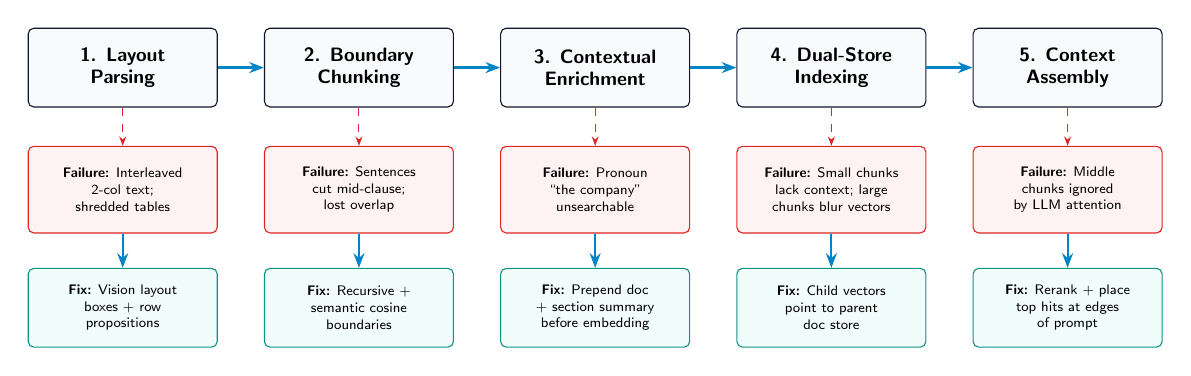
\begin{tikzpicture}[
  stage/.style={draw=headingblue, fill=codebg, rounded corners=2pt, font=\sffamily\scriptsize\bfseries, minimum width=2.4cm, minimum height=1.0cm, align=center},
  fail/.style={draw=warningRed, fill=warningBg, rounded corners=2pt, font=\sffamily\tiny, minimum width=2.4cm, minimum height=1.1cm, align=center},
  fix/.style={draw=intuitionTeal, fill=intuitionBg, rounded corners=2pt, font=\sffamily\tiny, minimum width=2.4cm, minimum height=1.0cm, align=center},
  arrow/.style={-{Stealth[scale=0.8]}, thick, color=linkblue},
  farrow/.style={-{Stealth[scale=0.7]}, dashed, color=warningRed}
]

\node[stage] (s1) at (0,0) {1. Layout\\Parsing};
\node[stage] (s2) at (3.0,0) {2. Boundary\\Chunking};
\node[stage] (s3) at (6.0,0) {3. Contextual\\Enrichment};
\node[stage] (s4) at (9.0,0) {4. Dual-Store\\Indexing};
\node[stage] (s5) at (12.0,0) {5. Context\\Assembly};

\draw[arrow] (s1) -- (s2);
\draw[arrow] (s2) -- (s3);
\draw[arrow] (s3) -- (s4);
\draw[arrow] (s4) -- (s5);

\node[fail] (f1) at (0,-1.55) {\textbf{Failure:} Interleaved\\2-col text;\\shredded tables};
\node[fail] (f2) at (3.0,-1.55) {\textbf{Failure:} Sentences\\cut mid-clause;\\lost overlap};
\node[fail] (f3) at (6.0,-1.55) {\textbf{Failure:} Pronoun\\``the company''\\unsearchable};
\node[fail] (f4) at (9.0,-1.55) {\textbf{Failure:} Small chunks\\lack context; large\\chunks blur vectors};
\node[fail] (f5) at (12.0,-1.55) {\textbf{Failure:} Middle\\chunks ignored\\by LLM attention};

\node[fix] (x1) at (0,-3.05) {\textbf{Fix:} Vision layout\\boxes + row\\propositions};
\node[fix] (x2) at (3.0,-3.05) {\textbf{Fix:} Recursive +\\semantic cosine\\boundaries};
\node[fix] (x3) at (6.0,-3.05) {\textbf{Fix:} Prepend doc\\+ section summary\\before embedding};
\node[fix] (x4) at (9.0,-3.05) {\textbf{Fix:} Child vectors\\point to parent\\doc store};
\node[fix] (x5) at (12.0,-3.05) {\textbf{Fix:} Rerank + place\\top hits at edges\\of prompt};

\draw[farrow] (s1) -- (f1); \draw[arrow] (f1) -- (x1);
\draw[farrow] (s2) -- (f2); \draw[arrow] (f2) -- (x2);
\draw[farrow] (s3) -- (f3); \draw[arrow] (f3) -- (x3);
\draw[farrow] (s4) -- (f4); \draw[arrow] (f4) -- (x4);
\draw[farrow] (s5) -- (f5); \draw[arrow] (f5) -- (x5);

\end{tikzpicture}
\caption{Production RAG Data Flow, Stage-Specific Failure Modes, and Architectural Mitigations.}
\label{fig:v2-ch02-rag-failure-map}
\end{figure}

Notice the core lesson of Figure~\ref{fig:v2-ch02-rag-failure-map}: if Stages 1--3 shred a table or strip away an entity name, Stage 5 cannot guess the missing facts later. High-accuracy RAG is won at ingestion time.

\section{Document Parsing and Structural Extraction}

\subsection{Why Raw PDF Text Streams Fail}
PDF is a print-drawing format, not a structured text format. Internally, a PDF stores painting commands placed at $(x, y)$ page coordinates:
\begin{equation}
(x=72,\; y=640,\; \text{``Consolidated''},\; \text{Helvetica},\; 10\text{pt})
\end{equation}
A PDF has no built-in tags for ``paragraph,'' ``column,'' or ``table.'' When a naive text extractor walks the stream left-to-right across a two-column financial report, it stitches Column A's line directly into Column B's line:
\begin{center}
\emph{``In 2024 our European division grew 14\%''} $\longleftrightarrow$ \emph{``While regulatory filings remained pending.''}
\end{center}

\begin{underthehoodbox}[Vision-Based Layout Analysis]
Modern document parsers (such as Marker, Docling, or LayoutLMv3) treat pages visually before reading strings:
\begin{enumerate}
  \item Render each PDF page into a bitmap image (e.g., 150--300 DPI).
  \item Run an object-detection model to draw bounding boxes labeled \texttt{Heading}, \texttt{Paragraph}, \texttt{Table}, \texttt{Header}, and \texttt{Footer}.
  \item Sort bounding boxes into true reading order (top-to-bottom within Column 1, then Column 2), drop repeated page headers/footers, and extract text inside each box via native PDF glyphs or OCR.
  \item Emit a clean Markdown hierarchy preserving headings and tables.
\end{enumerate}
\end{underthehoodbox}

\subsection{Flattening Tables into Self-Contained Propositions}
If a raw pipe-delimited Markdown table spans 40 rows and gets split at row 15, rows 16--40 lose their header row (\texttt{Year | Revenue | OpEx | EBITDA}) and become meaningless numbers. A reliable solution converts each row into a self-contained sentence (Listing~\ref{lst:v2-ch02-tables}).

\begin{lstlisting}[language=Python, label={lst:v2-ch02-tables}, caption={Flattening Financial Table Rows into Self-Contained Propositions}]
def table_to_context_tuples(table_data: list[dict[str, str]]) -> list[str]:
    """Flattens structured table rows into standalone sentences."""
    propositions: list[str] = []
    for row in table_data:
        prop = (
            f"In financial year {row['Year']}, the company recorded revenue "
            f"of {row['Revenue']}, operating expenses of {row['OpEx']}, "
            f"yielding an EBITDA of {row['EBITDA']}."
        )
        propositions.append(prop)
    return propositions

# Trace on a 2-row sample:
rows = [
    {"Year": "2023", "Revenue": "$120M", "OpEx": "$80M", "EBITDA": "$40M"},
    {"Year": "2024", "Revenue": "$150M", "OpEx": "$95M", "EBITDA": "$55M"},
]
# Output[0]: "In financial year 2023, the company recorded revenue of $120M,
#             operating expenses of $80M, yielding an EBITDA of $40M."
\end{lstlisting}

Each emitted string now carries its own column labels, so even if two rows land in separate chunks, neither loses its meaning.

\section{Chunking Topologies: Fixed, Recursive, and Semantic}

\subsection{Tokens vs Characters: A Quick Primer}
Before measuring chunk sizes, clarify what LLMs actually count. Language models do not read raw characters or whole English words; a \textbf{tokenizer} (typically Byte-Pair Encoding, or BPE) slices text into common subword pieces called \textbf{tokens}. For example, \texttt{"unbelievable"} might become \texttt{["un", "believ", "able"]} (3 tokens). As a rule of thumb:
\begin{itemize}[leftmargin=18pt]
  \item In English prose, $1\text{ token} \approx 4\text{ characters}$.
  \item In source code or JSON (heavy indentation, symbols, camelCase), $1\text{ token} \approx 2.5\text{ to }3.0\text{ characters}$.
\end{itemize}

\begin{figure}[htbp]
\centering
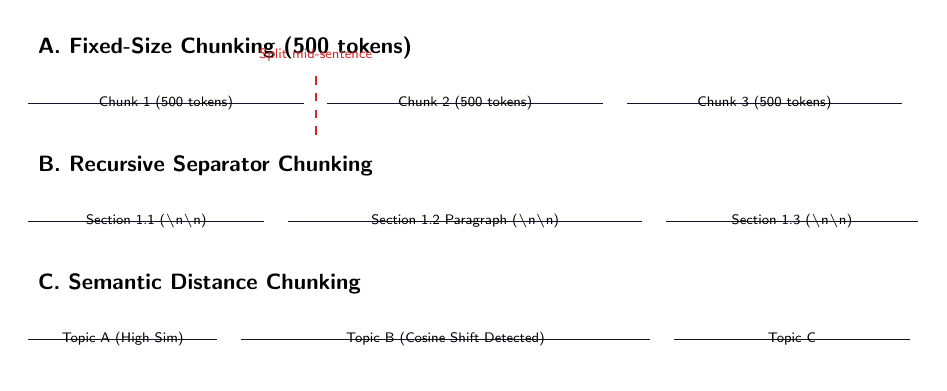
\begin{tikzpicture}[
  chunk/.style={draw=headingblue, fill=codebg, rounded corners=1pt, minimum height=0.6cm, font=\sffamily\tiny, align=center},
  sep/.style={draw=warningRed, dashed, thick}
]

\node[anchor=west, font=\sffamily\bfseries\footnotesize] at (0, 2.2) {A. Fixed-Size Chunking (500 tokens)};
\draw[chunk, minimum width=3.5cm] (0, 1.5) -- ++(3.5,0) node[midway] {Chunk 1 (500 tokens)};
\draw[chunk, minimum width=3.5cm] (3.8, 1.5) -- ++(3.5,0) node[midway] {Chunk 2 (500 tokens)};
\draw[chunk, minimum width=3.5cm] (7.6, 1.5) -- ++(3.5,0) node[midway] {Chunk 3 (500 tokens)};
\draw[sep] (3.65, 1.1) -- (3.65, 1.9) node[above, font=\tiny\sffamily, color=warningRed] {Split mid-sentence};

\node[anchor=west, font=\sffamily\bfseries\footnotesize] at (0, 0.7) {B. Recursive Separator Chunking};
\draw[chunk, minimum width=3.0cm, fill=intuitionBg] (0, 0) -- ++(3.0,0) node[midway] {Section 1.1 ($\backslash$n$\backslash$n)};
\draw[chunk, minimum width=4.5cm, fill=intuitionBg] (3.3, 0) -- ++(4.5,0) node[midway] {Section 1.2 Paragraph ($\backslash$n$\backslash$n)};
\draw[chunk, minimum width=3.2cm, fill=intuitionBg] (8.1, 0) -- ++(3.2,0) node[midway] {Section 1.3 ($\backslash$n$\backslash$n)};

\node[anchor=west, font=\sffamily\bfseries\footnotesize] at (0, -0.8) {C. Semantic Distance Chunking};
\draw[chunk, minimum width=2.4cm, fill=exampleBg] (0, -1.5) -- ++(2.4,0) node[midway] {Topic A (High Sim)};
\draw[chunk, minimum width=5.2cm, fill=exampleBg] (2.7, -1.5) -- ++(5.2,0) node[midway] {Topic B (Cosine Shift Detected)};
\draw[chunk, minimum width=3.0cm, fill=exampleBg] (8.2, -1.5) -- ++(3.0,0) node[midway] {Topic C};

\end{tikzpicture}
\caption{Chunking Topologies: Fixed slicing breaks mid-sentence; recursive splitting honors document separators; semantic chunking splits when embedding similarity drops.}
\label{fig:v2-ch02-chunking}
\end{figure}

\subsection{Recursive Character Splitting (Done Right)}
Recursive splitting tries a prioritized list of natural boundaries—paragraphs (\texttt{"\textbackslash n\textbackslash n"}), lines (\texttt{"\textbackslash n"}), sentences (\texttt{". "}), clauses (\texttt{"; "}), words (\texttt{" "}), and finally raw characters (\texttt{""})—as illustrated in Figure~\ref{fig:v2-ch02-chunking}B.

A classic bug in naive implementations is computing \texttt{new\_separators = separators[i+1:]} and forgetting to \emph{recurse} when an oversized paragraph is encountered, or forgetting to include \texttt{len(separator)} when budgeting overlap. Listing~\ref{lst:v2-ch02-recursive} fixes both bugs cleanly.

\begin{lstlisting}[language=Python, label={lst:v2-ch02-recursive}, caption={Production Recursive Separator Splitter with True Recursion and Exact Overlap}]
import re

class ProductionRecursiveSplitter:
    def __init__(self, chunk_size: int = 1000, chunk_overlap: int = 150):
        self.chunk_size = chunk_size
        self.chunk_overlap = chunk_overlap
        self.separators = ["\n\n", "\n", ". ", "; ", ", ", " ", ""]

    def split_text(self, text: str) -> list[str]:
        def _split(txt: str, separators: list[str]) -> list[str]:
            if len(txt) <= self.chunk_size:
                return [txt] if txt.strip() else []

            separator = separators[-1]
            new_separators: list[str] = []
            for i, sep in enumerate(separators):
                if sep == "":
                    separator = ""
                    break
                if re.search(re.escape(sep), txt):
                    separator = sep
                    new_separators = separators[i + 1:]
                    break

            splits = txt.split(separator) if separator else list(txt)
            docs: list[str] = []
            current_doc: list[str] = []
            current_len = 0

            def _flush() -> None:
                nonlocal current_doc, current_len
                if not current_doc:
                    return
                merged = separator.join(current_doc)
                if merged.strip():
                    docs.append(merged)
                overlap_doc: list[str] = []
                overlap_len = 0
                for prev_s in reversed(current_doc):
                    added = len(prev_s) + (len(separator) if overlap_doc else 0)
                    if overlap_len + added > self.chunk_overlap:
                        break
                    overlap_doc.insert(0, prev_s)
                    overlap_len += added
                current_doc = overlap_doc
                current_len = overlap_len

            for s in splits:
                if len(s) > self.chunk_size:
                    _flush()
                    current_doc, current_len = [], 0
                    if new_separators:
                        docs.extend(_split(s, new_separators))
                    else:
                        step = max(1, self.chunk_size - self.chunk_overlap)
                        for start in range(0, len(s), step):
                            part = s[start:start + self.chunk_size]
                            if part.strip():
                                docs.append(part)
                    continue

                sep_len = len(separator) if current_doc else 0
                if current_len + sep_len + len(s) > self.chunk_size:
                    _flush()
                    sep_len = len(separator) if current_doc else 0
                    if current_len + sep_len + len(s) > self.chunk_size:
                        current_doc, current_len, sep_len = [], 0, 0

                current_doc.append(s)
                current_len += sep_len + len(s)

            if current_doc:
                merged = separator.join(current_doc)
                if merged.strip():
                    docs.append(merged)
            return docs

        return _split(text, self.separators)
\end{lstlisting}

\textbf{Step-by-Step Walkthrough on a Concrete Input:} Configure \texttt{chunk\_size=80, chunk\_overlap=20} and pass:
\begin{quote}\small\ttfamily
"Section 1: Overview. Maintain liquidity.\textbackslash n\textbackslash nSection 2: Covenants. EBITDA must exceed \$50M. The debt ratio shall not exceed 3.5:1.0.\textbackslash n\textbackslash nSection 3: Remedies."
\end{quote}
\begin{enumerate}[leftmargin=18pt]
  \item Line 11 checks \texttt{len(txt) <= 80} (False, 177 chars). Lines 16--23 match the highest-priority separator \texttt{"\textbackslash n\textbackslash n"} and set \texttt{new\_separators = ["\textbackslash n", ". ", "; ", ", ", " ", ""]}.
  \item Line 25 splits into three paragraphs: $p_0$ (42 chars), $p_1$ (92 chars), and $p_2$ (20 chars).
  \item $p_0$ (42 chars $\le 80$) enters \texttt{current\_doc}. Next comes $p_1$ (92 chars $> 80$). Line 49 catches \texttt{len(s) > chunk\_size}, flushes $p_0$ as Chunk 0, clears the buffer, and calls \texttt{\_split(p\_1, new\_separators)} at line 53!
  \item Inside the recursive call on $p_1$, \texttt{"\textbackslash n"} is absent, so line 20 selects \texttt{". "} and splits into three sentences: \texttt{"Section 2: Covenants"} (20), \texttt{"EBITDA must exceed \$50M"} (23), and \texttt{"The debt ratio shall not exceed 3.5:1.0."} (40). The first two join with \texttt{". "} to 45 chars; adding the third ($45 + 2 + 40 = 87 > 80$) triggers \texttt{\_flush()}. In \texttt{\_flush()}, \texttt{overlap\_doc} retains \texttt{"EBITDA must exceed \$50M"} (23 chars $> 20$? Wait: $23 > 20$, so overlap stops at 0 if overlap=20, or retains it if \texttt{chunk\_overlap=25}—and crucially line 40 accounts for \texttt{len(separator)} whenever two retained segments are joined!).
  \item Every emitted chunk is guaranteed to obey \texttt{len(chunk) <= 80} while preserving sentence boundaries.
\end{enumerate}

\subsection{Semantic Chunking: A Worked 4-Sentence Example}
Even recursive splitting cuts blindly between paragraphs that discuss the same topic, or merges two unrelated paragraphs that happen to fit under \texttt{chunk\_size}. \textbf{Semantic chunking} splits when the meaning shifts between consecutive sentences.

Suppose a runbook contains 4 sentences:
\begin{itemize}[leftmargin=18pt]
  \item $s_0$: \emph{``PostgreSQL records every data change in the Write-Ahead Log before modifying heap pages.''}
  \item $s_1$: \emph{``If the server loses power, WAL replay restores committed transactions safely.''}
  \item $s_2$: \emph{``Kubernetes Horizontal Pod Autoscalers monitor CPU utilization every 15 seconds.''}
  \item $s_3$: \emph{``When load exceeds the target threshold, the controller adds new pod replicas.''}
\end{itemize}
Suppose we embed each sentence (or 3-sentence sliding window) and compute cosine similarity between consecutive pairs using Chapter~1's formula, obtaining:
\[
S_{\cos}(s_0, s_1) = 0.88, \qquad S_{\cos}(s_1, s_2) = 0.42, \qquad S_{\cos}(s_2, s_3) = 0.85
\]
Converting similarities to cosine distances $D_i = 1 - S_{\cos}(s_i, s_{i+1})$ gives:
\[
D = [D_0, D_1, D_2] = [0.12,\; 0.58,\; 0.15]
\]
Compute the statistics of $D$:
\[
\mu_D = \frac{0.12 + 0.58 + 0.15}{3} \approx 0.2833, \qquad \sigma_D = \sqrt{\frac{(0.12-0.2833)^2 + (0.58-0.2833)^2 + (0.15-0.2833)^2}{3}} \approx 0.2101
\]
Using an 85th-percentile cutoff (linearly interpolated on sorted $[0.12, 0.15, 0.58]$ at index $0.85 \times 2 = 1.7$, giving $\text{cutoff} = 0.15 + 0.7(0.58 - 0.15) = 0.451$), or equivalently $\tau = \mu_D + 0.8\sigma_D \approx 0.4514$:
\begin{itemize}[leftmargin=18pt]
  \item $D_0 = 0.12 \le 0.451 \implies$ keep $s_0$ and $s_1$ together.
  \item $D_1 = 0.58 > 0.451 \implies$ \textbf{topic jump detected!} Split between $s_1$ and $s_2$.
  \item $D_2 = 0.15 \le 0.451 \implies$ keep $s_2$ and $s_3$ together.
\end{itemize}
Result: Chunk 1 = $\{s_0, s_1\}$ (PostgreSQL WAL) and Chunk 2 = $\{s_2, s_3\}$ (Kubernetes HPA). Listing~\ref{lst:v2-ch02-semantic} implements this exact pass.

\begin{lstlisting}[language=Python, label={lst:v2-ch02-semantic}, caption={Semantic Chunking via Adjacent Cosine Distance}]
import numpy as np

def semantic_chunking(
    sentences: list[str],
    embeddings: np.ndarray,
    threshold_percentile: float = 85.0
) -> list[str]:
    """Splits sentences into chunks where embedding distance spikes."""
    if len(sentences) <= 1:
        return sentences

    # embeddings shape: (N, D), pre-normalized to unit length
    distances = np.array([
        1.0 - float(np.dot(embeddings[i], embeddings[i + 1]))
        for i in range(len(embeddings) - 1)
    ])
    cutoff = float(np.percentile(distances, threshold_percentile))

    chunks: list[str] = []
    current_chunk = [sentences[0]]
    for i, dist in enumerate(distances):
        if dist > cutoff:
            chunks.append(" ".join(current_chunk))
            current_chunk = [sentences[i + 1]]
        else:
            current_chunk.append(sentences[i + 1])

    if current_chunk:
        chunks.append(" ".join(current_chunk))
    return chunks
\end{lstlisting}

\section{The ``Lost in the Middle'' Phenomenon}

Even if chunking is spotless, pasting 30 retrieved chunks into a 64k-token prompt backfires. Liu et al. (2023) showed that LLM accuracy forms a U-shaped curve (Figure~\ref{fig:v2-ch02-lost-middle}): models reliably use facts at the very start (\textbf{primacy}) and very end (\textbf{recency}) of the prompt, while accuracy drops by 30--50\% when the critical answer sits in the middle.

\begin{figure}[htbp]
\centering
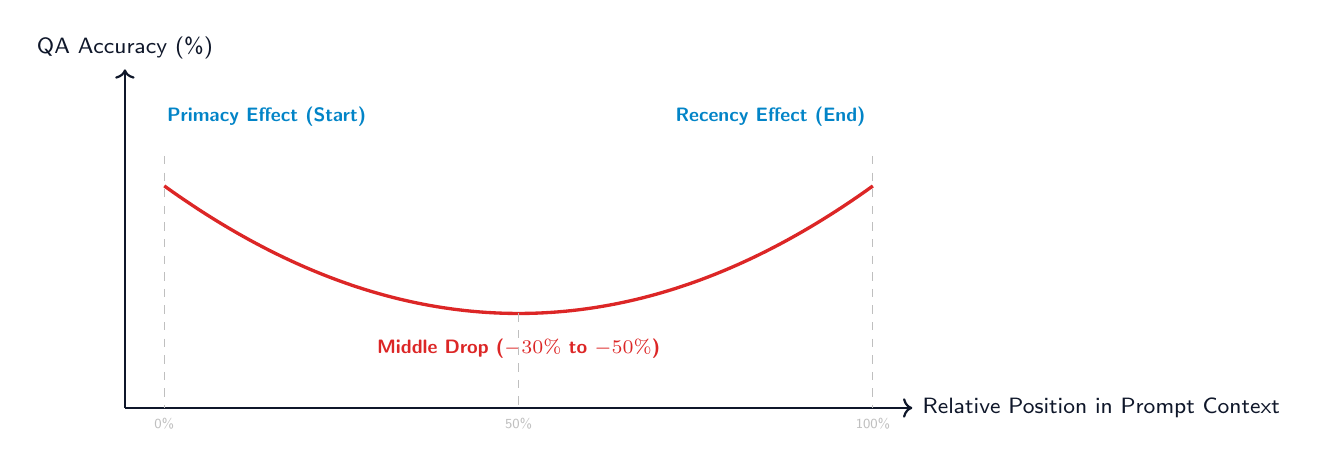
\begin{tikzpicture}
\draw[->, thick, color=headingblue] (0,0) -- (10,0) node[right, font=\sffamily\footnotesize] {Relative Position in Prompt Context};
\draw[->, thick, color=headingblue] (0,0) -- (0,4.3) node[above, font=\sffamily\footnotesize] {QA Accuracy (\%)};

\draw[very thick, color=warningRed, domain=0.5:9.5, samples=100]
  plot (\x, {0.08*(\x - 5.0)*(\x - 5.0) + 1.2});

\node[font=\sffamily\scriptsize\bfseries, color=linkblue] at (1.8, 3.7) {Primacy Effect (Start)};
\node[font=\sffamily\scriptsize\bfseries, color=linkblue] at (8.2, 3.7) {Recency Effect (End)};
\node[font=\sffamily\scriptsize\bfseries, color=warningRed] at (5.0, 0.75) {Middle Drop ($-30\%$ to $-50\%$)};

\draw[dashed, color=gray!50] (0.5, 3.2) -- (0.5, 0) node[below, font=\tiny\sffamily] {0\%};
\draw[dashed, color=gray!50] (5.0, 1.2) -- (5.0, 0) node[below, font=\tiny\sffamily] {50\%};
\draw[dashed, color=gray!50] (9.5, 3.2) -- (9.5, 0) node[below, font=\tiny\sffamily] {100\%};

\end{tikzpicture}
\caption{The ``Lost in the Middle'' U-Shaped Attention Curve: Information buried near the center of a long prompt receives weaker attention than chunks placed near the start or end.}
\label{fig:v2-ch02-lost-middle}
\end{figure}

\begin{underthehoodbox}[Why Does This Happen? Attention Decay, RoPE, and Attention Sinks]
When an LLM generates the next word, its \textbf{self-attention} mechanism assigns a numerical weight (summing to 1.0) across all earlier tokens in the prompt to decide which ones matter right now. Two mechanics starve middle tokens:
\begin{enumerate}
  \item \textbf{Rotary Position Embeddings (RoPE) Distance Decay}: To tell whether one word is 5 tokens away or 20,000 tokens away, modern LLMs encode position by rotating each token's internal vector in 2D planes by an angle proportional to its position index. As the gap $|i - j|$ between a middle chunk and the end of the prompt stretches across tens of thousands of tokens, relative alignment decays and long-range attention blurs.
  \item \textbf{Attention Sinks and Recency}: Tokens at the very end sit immediately next to the freshly generated output, dominating recency weights. Meanwhile, the very first tokens (token 0, the system prompt) act as an \textbf{attention sink}: because attention weights must sum to 1.0 even when no specific word is strongly relevant, models dump spare attention weight onto the opening tokens, leaving middle tokens starved.
\end{enumerate}
\end{underthehoodbox}

\begin{productionwarningbox}[The Context-Stuffing Anti-Pattern]
Upgrading from an 8k-token model to a 128k-token model does not fix poor retrieval. Dumping 40 raw chunks into a prompt buries the best evidence in the middle and inflates latency and cost. Keep retrieved context tight (top 5--8 chunks after reranking, Chapter~3), deduplicate overlapping chunks, and place your highest-scoring chunks at the top and bottom of the context block.
\end{productionwarningbox}

\section{Small-to-Big Retrieval and Contextual Enrichment}

\subsection{Parent-Document Retrieval: Decoupling Search from Generation}
Chunk size creates a tug-of-war:
\begin{itemize}[leftmargin=18pt]
  \item \textbf{Small chunks (100--150 tokens)} produce razor-sharp vectors because each vector describes one focused fact.
  \item \textbf{Large chunks (1,000--1,500 tokens)} give the LLM full surrounding clauses, definitions, and tables.
\end{itemize}
\textbf{Parent-Document Retrieval} solves both by indexing small \emph{child} chunks in the vector database while storing the large \emph{parent} section in a key-value store (Figure~\ref{fig:v2-ch02-parent}).

\begin{figure}[htbp]
\centering
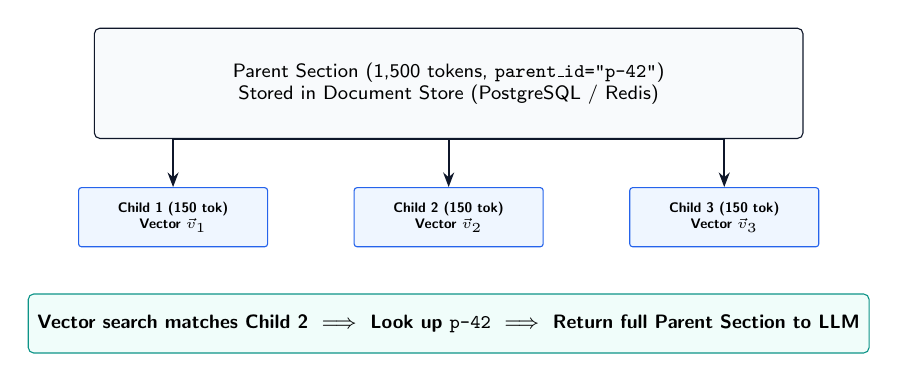
\begin{tikzpicture}[
  parent/.style={draw=headingblue, fill=codebg, rounded corners=2pt, minimum width=9.0cm, minimum height=1.4cm, font=\sffamily\scriptsize, align=center},
  child/.style={draw=exampleBlue, fill=exampleBg, rounded corners=1pt, minimum width=2.4cm, minimum height=0.75cm, font=\sffamily\tiny\bfseries, align=center},
  arrow/.style={-{Stealth[scale=0.8]}, thick, color=headingblue}
]

\node[parent] (p1) at (5, 2.4) {Parent Section (1,500 tokens, \texttt{parent\_id="p-42"})\\Stored in Document Store (PostgreSQL / Redis)};
\node[child] (c1) at (1.5, 0.7) {Child 1 (150 tok)\\Vector $\vec{v}_1$};
\node[child] (c2) at (5.0, 0.7) {Child 2 (150 tok)\\Vector $\vec{v}_2$};
\node[child] (c3) at (8.5, 0.7) {Child 3 (150 tok)\\Vector $\vec{v}_3$};

\draw[arrow] (p1.south) -| (c1.north);
\draw[arrow] (p1.south) -- (c2.north);
\draw[arrow] (p1.south) -| (c3.north);

\node[draw=intuitionTeal, fill=intuitionBg, rounded corners=2pt, font=\sffamily\scriptsize\bfseries, minimum width=9.0cm, minimum height=0.75cm] at (5, -0.65) {
  Vector search matches Child 2 $\implies$ Look up \texttt{p-42} $\implies$ Return full Parent Section to LLM
};

\end{tikzpicture}
\caption{Parent-Document (Small-to-Big) Retrieval: Granular child vectors maximize search accuracy; deduplicated parent sections preserve full context for generation.}
\label{fig:v2-ch02-parent}
\end{figure}

\begin{lstlisting}[language=Python, label={lst:v2-ch02-parent}, caption={Parent-Document Retrieval with Ordered Parent Deduplication}]
import uuid

class ParentDocumentRetriever:
    def __init__(self, vector_store, doc_store: dict[str, str]):
        self.vector_store = vector_store
        self.doc_store = doc_store
        self.child_splitter = ProductionRecursiveSplitter(chunk_size=200, chunk_overlap=20)
        self.parent_splitter = ProductionRecursiveSplitter(chunk_size=1500, chunk_overlap=150)

    def add_documents(self, raw_documents: list[str]) -> None:
        for raw_doc in raw_documents:
            parents = self.parent_splitter.split_text(raw_doc)
            for parent_text in parents:
                parent_id = str(uuid.uuid4())
                self.doc_store[parent_id] = parent_text

                children = self.child_splitter.split_text(parent_text)
                for child_text in children:
                    metadata = {"parent_id": parent_id, "snippet": child_text[:50]}
                    self.vector_store.add_text(child_text, metadata=metadata)

    def retrieve(self, query: str, top_k_children: int = 10) -> list[str]:
        child_matches = self.vector_store.search(query, k=top_k_children)

        seen_parent_ids: set[str] = set()
        parent_documents: list[str] = []
        for match in child_matches:
            pid = match.metadata["parent_id"]
            if pid not in seen_parent_ids:
                seen_parent_ids.add(pid)
                parent_documents.append(self.doc_store[pid])
        return parent_documents
\end{lstlisting}

\textbf{Step-by-Step Trace of \texttt{ParentDocumentRetriever}:}
Suppose we ingest our bond indenture from the motivating problem:
\begin{enumerate}[leftmargin=18pt]
  \item \texttt{add\_documents} splits the indenture into 1,500-character parents (lines 12--15). Section 4.02 (Negative Covenants) gets \texttt{parent\_id = "p-402"} and its full text is saved in \texttt{self.doc\_store["p-402"]}.
  \item Lines 17--20 slice \texttt{"p-402"} into 200-character children: Child A mentions \emph{``Section 4.02 Negative Covenants: Consolidated EBITDA''}, Child B contains \emph{``...the ratio shall not exceed 3.5:1.0''}. Both carry \texttt{metadata=\{"parent\_id": "p-402"\}}.
  \item When the analyst queries \texttt{"debt ratio under negative covenants"}, line 23 returns Child B (rank 1, \texttt{parent\_id="p-402"}) and Child A (rank 2, \texttt{parent\_id="p-402"}), followed by Child C from Section 7.1 (\texttt{parent\_id="p-701"}).
  \item Lines 27--31 iterate in rank order: \texttt{"p-402"} is added once to \texttt{seen\_parent\_ids} and appended; when Child A arrives with the same \texttt{"p-402"}, line 29 skips the duplicate so the LLM receives Section 4.02 once—complete with its covenant header—followed by Section 7.1.
\end{enumerate}

\subsection{Contextual Retrieval: Eliminating Orphan Chunks}
Consider a standalone chunk from an SEC filing:
\begin{center}
\emph{``Operating margin declined by 2.4\% due to regulatory headwinds in the mobility segment.''}
\end{center}
Even with small chunks, a query asking \emph{``Why did Uber's Q3 2024 operating margin drop?''} fails if neither \emph{``Uber''} nor \emph{``Q3 2024''} appears inside the chunk! \textbf{Contextual Retrieval} (Anthropic, 2024) fixes this at ingestion time by asking a fast, low-cost LLM to prepend a 2-sentence situating prefix before embedding (Listing~\ref{lst:v2-ch02-contextual}).

\begin{lstlisting}[language=Python, label={lst:v2-ch02-contextual}, caption={Contextual Enrichment Prior to Vector Embedding}]
CONTEXT_ENRICHMENT_PROMPT = """<document>
{full_document}
</document>

Here is the chunk we want to situate within the whole document:
<chunk>
{chunk_text}
</chunk>

Give a short, concise context (2-3 sentences) to situate this chunk within the overall document for search retrieval. Answer ONLY with the context."""

async def generate_contextual_chunk(
    llm_client, full_document: str, chunk_text: str
) -> str:
    prompt = CONTEXT_ENRICHMENT_PROMPT.format(
        full_document=full_document[:20000],
        chunk_text=chunk_text
    )
    context_prefix = await llm_client.generate(prompt, max_tokens=100)
    return f"{context_prefix.strip()}\n\n{chunk_text}"
\end{lstlisting}

Prepending \emph{``This chunk is from Uber Technologies' Q3 2024 Form 10-Q discussing Mobility segment results.''} embeds \texttt{Uber}, \texttt{Q3 2024}, and \texttt{Form 10-Q} directly into the chunk vector—cutting retrieval failures by nearly half in production benchmarks, especially when paired with prompt caching (Chapter~7) so \texttt{full\_document} is cached across all chunks of the same file.

\begin{realworldbox}[Diagnosing Orphaned Pronoun \& Table-Header Failures]
An internal compliance assistant answered \emph{``I found no record of the Q3 margin change''} on 38\% of financial questions. Inspecting the retrieval trace exposed the culprit:
\begin{lstlisting}[basicstyle=\ttfamily\scriptsize]
TRACE query="What was Acme Corp's Q3 2024 operating margin?"
  top_1_hit (cos=0.61): "2024 | $150M | $95M | $55M"         # Missing header \& company!
  top_2_hit (cos=0.58): "The segment fell 2.4% vs prior yr." # Missing entity \& quarter!
\end{lstlisting}
The true table row had been split away from its header, and the narrative paragraph never repeated \emph{``Acme Corp''}. Flattening table rows into prose tuples (Listing~\ref{lst:v2-ch02-tables}) and prepending contextual prefixes (Listing~\ref{lst:v2-ch02-contextual}) lifted top-5 retrieval recall from 62\% to 94\%.
\end{realworldbox}

\begin{tryityourselfbox}[Tracing Recursive Splitting \& Overlap Calculation]
Trace \texttt{ProductionRecursiveSplitter(chunk\_size=50, chunk\_overlap=15)} on the input:
\begin{quote}\small\ttfamily
"Alpha one. Beta two. Gamma three.\textbackslash n\textbackslash nDelta four."
\end{quote}
List the exact output chunks, their character lengths, and explain which separator level handled each split. (Worked solution is in Section~2.7.)
\end{tryityourselfbox}

\section{Chapter Summary \protect\& Key Takeaways}
\begin{itemize}[leftmargin=18pt]
  \item \textbf{Structure-First Ingestion}: Use layout-aware parsers for multi-column PDFs and flatten tables into self-contained propositions so rows keep their headers.
  \item \textbf{Recursive \& Semantic Chunking}: True recursive splitters descend into finer separators whenever a segment exceeds \texttt{chunk\_size} and account for \texttt{len(separator)} during overlap; semantic chunkers detect topic shifts via spikes in adjacent cosine distance.
  \item \textbf{Lost in the Middle}: Due to RoPE distance decay, recency, and attention sinks, LLMs under-attend to the center of long prompts. Rerank and place top chunks at the edges.
  \item \textbf{Parent-Document \& Contextual Retrieval}: Search over small, focused child chunks, deduplicate \texttt{parent\_id}s, and return full parent sections; prepend document/section context before embedding to eliminate orphan pronouns.
\end{itemize}

\section{Exercises}

\subsection*{Mechanics}
\textbf{Exercise \thechapter.1}: A document has 10 sentences with adjacent cosine distances:
\[
D = [0.12,\; 0.15,\; 0.08,\; 0.45,\; 0.10,\; 0.11,\; 0.52,\; 0.09,\; 0.14]
\]
Given $\tau = \mu_D + 1.0 \cdot \sigma_D$, compute $\mu_D$, $\sigma_D$, and identify which sentence boundaries trigger splits.

\textbf{Exercise \thechapter.2}: Explain the difference between character overlap and token overlap. If a splitter sets \texttt{chunk\_overlap=100} characters on Python source code, approximately how many tokens of overlap does that produce?

\subsection*{Debugging}
\textbf{Exercise \thechapter.3}: After deploying \texttt{ParentDocumentRetriever}, an engineer notices that 5 out of 5 returned parent documents in the prompt are identical copies of the same 1,500-token section, crowding out all other evidence. Explain why this happens and write the Python deduplication fix.

\subsection*{Architecture}
\textbf{Exercise \thechapter.4}: Design an incremental ingestion pipeline for an enterprise wiki (Notion/Confluence) that updates parent and child records when a single page is edited, without leaving orphaned child vectors in the index.

\section{Detailed Solutions}

\subsection*{Solution \thechapter.1}
Count $N = 9$, sum $= 1.76$, so $\mu_D = 1.76 / 9 \approx 0.1956$. Computing squared deviations $(D_i - 0.1956)^2$:
\[
0.0057 + 0.0021 + 0.0134 + 0.0647 + 0.0091 + 0.0073 + 0.1052 + 0.0112 + 0.0031 = 0.2218
\]
Variance $\sigma_D^2 = 0.2218 / 9 \approx 0.02464 \implies \sigma_D \approx 0.1570$. Threshold $\tau = 0.1956 + 0.1570 = 0.3526$. Two distances exceed $\tau$: $D_3 = 0.45$ (split between $s_3$ and $s_4$) and $D_6 = 0.52$ (split between $s_6$ and $s_7$), yielding $\{s_0..s_3\}$, $\{s_4..s_6\}$, and $\{s_7..s_9\}$.

\subsection*{Solution \thechapter.2}
Character overlap counts raw characters (`len(s)`), whereas token overlap counts BPE subword pieces. In English prose, $1\text{ token} \approx 4\text{ chars}$; in code (punctuation, indentation, short identifiers), $1\text{ token} \approx 2.5\text{ to }3.0\text{ chars}$. Thus 100 characters of Python yields $\approx 100 / 2.8 \approx 35\text{--}40$ tokens.

\subsection*{Solution \thechapter.3}
Multiple child chunks from the same parent document ranked in the top 5 vector hits, each carrying the same \texttt{parent\_id}. Fetching \texttt{doc\_store[pid]} without tracking seen IDs repeats the parent 5 times. Fix:
\begin{lstlisting}[language=Python]
def deduplicate_parents(child_hits: list, doc_store: dict[str, str]) -> list[str]:
    seen: set[str] = set()
    parents: list[str] = []
    for hit in child_hits:
        pid = hit.metadata["parent_id"]
        if pid not in seen:
            seen.add(pid)
            parents.append(doc_store[pid])
    return parents
\end{lstlisting}

\subsection*{Solution \thechapter.4}
Key each parent and child deterministically by \texttt{sha256(doc\_id + ":" + str(version) + ":" + str(idx))}. On page update: (1) write the new parent and child vectors tagged with \texttt{doc\_id} and \texttt{version = v\_new}; (2) atomically update the pointer/metadata; (3) delete stale chunks with \texttt{DELETE FROM chunks WHERE doc\_id = :id AND version < :v\_new}; (4) route transient failures to a Dead-Letter Queue for idempotent retry.

\subsection*{Solution (Try It Yourself)}
First, top-level \texttt{\_split} splits on \texttt{"\textbackslash n\textbackslash n"} into $p_0 = \text{"Alpha one. Beta two. Gamma three."}$ (33 chars $\le 50$) and $p_1 = \text{"Delta four."}$ (11 chars $\le 50$). Adding $p_1$ to $p_0$ would reach $33 + 2 + 11 = 46 \le 50$, so wait: \texttt{"\textbackslash n\textbackslash n".join([p0, p1])} has length 46, fitting in a single 46-char chunk! If instead $p_0$ were 45 chars and $p_1$ were 11 chars ($45 + 2 + 11 = 58 > 50$), \texttt{\_flush()} emits $p_0$, checks overlap ($45 > 15$, so overlap is empty), and emits $p_1$ separately. (Testing edge cases like this with \texttt{len(separator)} included is why exact budget accounting matters!)

\begin{labbridgebox}[Hands-On Exercise \& Project Bridge]
Review how chunked documents feed dense cosine retrieval in \texttt{exercises/volume2/ex01\_vector\_math\_cosine.py}, and explore how retrieved text segments enter the hybrid search pipeline in \texttt{projects/p06-rag-hybrid-rerank/}.
\end{labbridgebox}

\section{Further Reading \protect\& Citations}
\begin{itemize}[leftmargin=18pt]
  \item Liu, N. F., et al. (2023). \emph{Lost in the Middle: How Language Models Use Long Contexts}. TACL.
  \item Anthropic. (2024). \emph{Introducing Contextual Retrieval}. Anthropic Research.
  \item Lewis, P., et al. (2020). \emph{Retrieval-Augmented Generation for Knowledge-Intensive NLP Tasks}. NeurIPS.
\end{itemize}

\chapter{Retrieval Algorithms and Reranking: Sparse, Dense, and Hybrid Fusion}
\label{chap:retrieval}

\begin{chaptergoalsbox}
\textbf{What You Will Learn:}
\begin{itemize}[leftmargin=15pt]
  \item Why pure dense vector search struggles with error codes, SKUs, and IP CIDRs.
  \item Building Okapi BM25 step-by-step: from raw word counts to TF-IDF, saturation ($k_1$), and document length normalization ($b$).
  \item Hybrid search fusion: why raw scores cannot be added directly and how Reciprocal Rank Fusion (RRF) merges ranked lists.
  \item Transformer encoder mechanics from scratch (\texttt{[CLS]}, \texttt{[SEP]}, $Q/K/V$ self-attention) and why Bi-Encoders ($O(\log N \cdot D)$ via HNSW) differ from Cross-Encoders.
  \item Two-stage retrieval cascades, Hypothetical Document Embeddings (HyDE), and Mean Reciprocal Rank (\texttt{MRR@K}).
\end{itemize}

\textbf{What You Should Already Understand:}
\begin{itemize}[leftmargin=15pt]
  \item Vectors, cosine similarity, and HNSW graph search (Chapter~1).
  \item Chunking and subword tokenization (Chapter~2).
\end{itemize}

\textbf{Why This Topic Exists:}
Dense vectors shine at paraphrases (\emph{``cardiac arrest''} $\leftrightarrow$ \emph{``heart attack''}), yet routinely fail when an engineer searches for an exact identifier such as \texttt{0x80070005}, \texttt{SKU-9921-X}, or \texttt{RFC 7540}. Production search combines exact lexical matching, semantic embeddings, and deep neural rerankers into a latency-budgeted cascade.

\textbf{Motivating Practical Problem:}
An internal SRE search portal indexes 250,000 incident post-mortems. During an outage, an on-call engineer searches \emph{``AWS ALB-502-BadGateway on subnet 10.240.12.0/24''}. Pure dense vector search returns generic documentation about HTTP 502 proxies and misses the exact post-mortem documenting the broken target-group health check on \texttt{10.240.12.0/24}, adding 45 minutes to Mean Time to Recovery (MTTR).
\end{chaptergoalsbox}

\section{Why Pure Dense Vectors Miss Exact Identifiers}

Dense embeddings compress a 300-word chunk into a single point in $\mathbb{R}^{1536}$. That compression deliberately discards exact surface spelling to capture general meaning, causing three failure modes:
\begin{enumerate}[leftmargin=18pt]
  \item \textbf{Tokenizer Fragmentation}: Rare codes like \texttt{0x80070005} get sliced by BPE into generic fragments (\texttt{['0', 'x', '80', '07', '00', '05']}) whose vector looks like any other hex string.
  \item \textbf{Near-Neighbor Collision}: In semantic space, \texttt{Product Model X-200} and \texttt{Product Model X-300} sit at cosine similarity $0.98$, even though their replacement parts are completely incompatible.
  \item \textbf{Query-Document Asymmetry}: Queries are short fragments (3--7 words) while documents are long prose (300--1,000 tokens).
\end{enumerate}

To restore exact-match precision, production engines run \textbf{lexical (keyword) search} alongside dense search.

\section{Building Okapi BM25 from First Principles}

Instead of jumping straight to a intimidating formula, build the scoring function of \textbf{Okapi BM25} (Robertson \& Zaragoza, 2009) in four logical steps on a tiny 3-document corpus for the query \texttt{"alb 502"}:
\begin{itemize}[leftmargin=18pt]
  \item $d_1$ (9 tokens): \texttt{"alb 502 error on subnet 10 240 12 0"}
  \item $d_2$ (8 tokens): \texttt{"http 502 gateway proxy overview and timeout guide"}
  \item $d_3$ (9 tokens): \texttt{"alb alb alb alb health check failed on subnet"}
\end{itemize}

\subsection*{Step 1: Raw Word Counts (Fails on Spam and Common Words)}
If we just count matching words, $d_1$ matches \texttt{alb} (1) + \texttt{502} (1) $= 2$, while $d_3$ matches \texttt{alb} (4) + \texttt{502} (0) $= 4$! Repeating one keyword four times lets $d_3$ outscore $d_1$, even though $d_3$ never mentions \texttt{502}.

\subsection*{Step 2: Inverse Document Frequency (TF-IDF)}
Common words appearing in almost every document (like \texttt{"the"} or \texttt{"error"}) carry less signal than rare words. \textbf{Inverse Document Frequency (IDF)} downweights ubiquitous words using the total document count $N$ and the number of documents $n(q)$ containing term $q$:
\begin{equation}
\text{IDF}(q) = \ln \left( \frac{N - n(q) + 0.5}{n(q) + 0.5} + 1 \right)
\end{equation}
In our 3-document corpus ($N = 3$), both \texttt{alb} and \texttt{502} appear in $n = 2$ documents, giving $\text{IDF} = \ln((3 - 2 + 0.5)/(2 + 0.5) + 1) = \ln(1.6) \approx 0.4700$. A stopword appearing in all 3 documents drops to $\ln(0.5/3.5 + 1) \approx 0.1335$, while a rare error code appearing in only 1 out of 1,000 documents jumps to $\approx 6.91$.

\subsection*{Step 3: Term Frequency Saturation ($k_1$)}
Mentioning \texttt{alb} twice tells us a little more than mentioning it once, but mentioning it 50 times is spam—not $50\times$ more relevant. BM25 caps the term-frequency bonus using a curve controlled by $k_1$ (typically $1.2 \le k_1 \le 2.0$):
\[
\text{TF\_sat}(f) = \frac{f \cdot (k_1 + 1)}{f + k_1}
\]
When $f = 1$, $\text{TF\_sat}(1) = 1.0$. As $f \to \infty$, $\text{TF\_sat}(f)$ flattens out at $k_1 + 1$ (Figure~\ref{fig:v2-ch03-bm25}). With $k_1 = 1.5$, seeing \texttt{alb} 4 times instead of 1 time lifts the term weight from $1.0$ to $\frac{4 \times 2.5}{4 + 1.5} = 1.818$ (not $4.0$!), neutralizing keyword stuffing.

\subsection*{Step 4: Document Length Normalization ($b$)}
A 2,000-word manual naturally accumulates more accidental word matches than a 40-word runbook. BM25 compares each document's length $|D|$ against the corpus average $\text{avgdl}$ using parameter $b \in [0, 1]$ (default $b = 0.75$):
\begin{equation}
\text{Score}_{\text{BM25}}(D, Q) = \sum_{i=1}^n \text{IDF}(q_i) \cdot \frac{f(q_i, D) \cdot (k_1 + 1)}{f(q_i, D) + k_1 \cdot \left(1 - b + b \cdot \frac{|D|}{\text{avgdl}}\right)}
\end{equation}
On our 3-document example ($\text{avgdl} = 8.667$, $k_1 = 1.5$, $b = 0.75$), $d_1$ scores $\mathbf{0.9240}$, $d_3$ scores $0.8479$, and $d_2$ scores $0.4869$—ranking $d_1$ first as desired!

\begin{figure}[htbp]
\centering
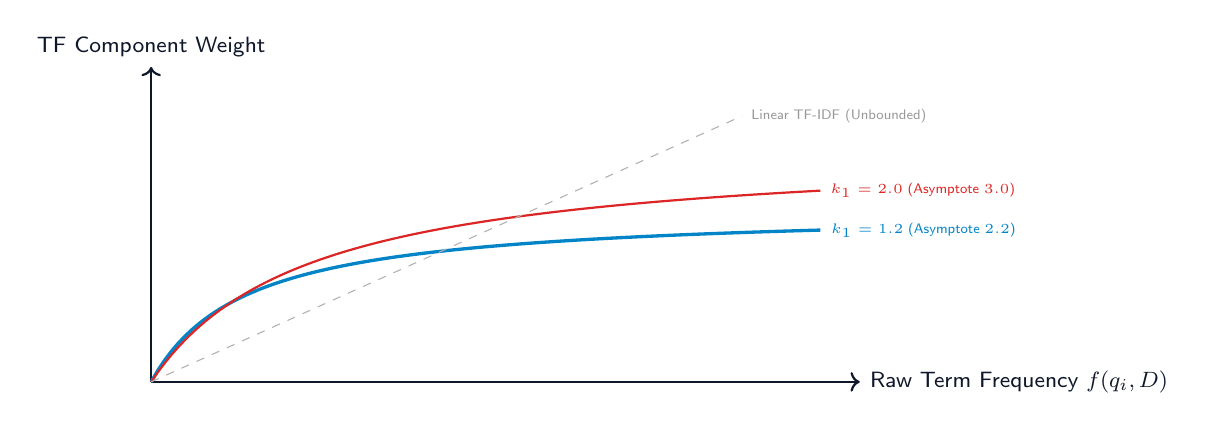
\begin{tikzpicture}
\draw[->, thick, color=headingblue] (0,0) -- (9,0) node[right, font=\sffamily\footnotesize] {Raw Term Frequency $f(q_i, D)$};
\draw[->, thick, color=headingblue] (0,0) -- (0,4) node[above, font=\sffamily\footnotesize] {TF Component Weight};

\draw[very thick, color=linkblue, domain=0:8.5, samples=100]
  plot (\x, {(\x * 2.2) / (\x + 1.2)})
  node[right, font=\tiny\sffamily, color=linkblue] {$k_1 = 1.2$ (Asymptote $2.2$)};

\draw[thick, color=warningRed, domain=0:8.5, samples=100]
  plot (\x, {(\x * 3.0) / (\x + 2.0)})
  node[right, font=\tiny\sffamily, color=warningRed] {$k_1 = 2.0$ (Asymptote $3.0$)};

\draw[dashed, color=gray!60, domain=0:7.5]
  plot (\x, {0.45 * \x})
  node[right, font=\tiny\sffamily, color=gray!80] {Linear TF-IDF (Unbounded)};

\end{tikzpicture}
\caption{BM25 Term Frequency Saturation: Unlike linear TF-IDF, BM25 approaches a horizontal ceiling $k_1 + 1$, preventing repeated-keyword spam from dominating results.}
\label{fig:v2-ch03-bm25}
\end{figure}

Listing~\ref{lst:v2-ch03-bm25} implements BM25 cleanly with both a low-level \texttt{.score()} method and a \texttt{.search()} method returning ranked document IDs.

\begin{lstlisting}[language=Python, label={lst:v2-ch03-bm25}, caption={Okapi BM25 Sparse Search Engine from First Principles}]
import math
import re
from collections import Counter

class ProductionBM25:
    def __init__(self, docs: dict[str, str], k1: float = 1.5, b: float = 0.75):
        self.k1 = k1
        self.b = b
        self.doc_ids = list(docs.keys())
        self.corpus_size = len(self.doc_ids)
        tokenized = [re.findall(r"\b\w+\b", docs[did].lower()) for did in self.doc_ids]
        self.doc_lens = [len(toks) for toks in tokenized]
        self.avgdl = sum(self.doc_lens) / max(1, self.corpus_size)

        self.df: Counter[str] = Counter()
        self.doc_freqs: list[Counter[str]] = []
        for toks in tokenized:
            counts = Counter(toks)
            self.doc_freqs.append(counts)
            for term in counts:
                self.df[term] += 1

        self.idf: dict[str, float] = {
            term: math.log((self.corpus_size - freq + 0.5) / (freq + 0.5) + 1.0)
            for term, freq in self.df.items()
        }

    def score(self, query_tokens: list[str]) -> list[float]:
        scores = [0.0] * self.corpus_size
        for term in query_tokens:
            if term not in self.idf:
                continue
            term_idf = self.idf[term]
            for idx, counts in enumerate(self.doc_freqs):
                tf = counts.get(term, 0)
                if tf == 0:
                    continue
                norm = 1.0 - self.b + self.b * (self.doc_lens[idx] / self.avgdl)
                scores[idx] += term_idf * (tf * (self.k1 + 1.0)) / (tf + self.k1 * norm)
        return scores

    def search(self, query: str, k: int = 100) -> list[str]:
        q_tokens = re.findall(r"\b\w+\b", query.lower())
        raw_scores = self.score(q_tokens)
        ranked = sorted(
            zip(self.doc_ids, raw_scores), key=lambda item: item[1], reverse=True
        )
        return [doc_id for doc_id, s in ranked[:k] if s > 0.0]
\end{lstlisting}

\section{Hybrid Fusion: Reciprocal Rank Fusion (RRF)}

Suppose BM25 returns unbounded positive scores like $14.2$ and $8.7$, while dense vector search returns cosine similarities in $[0.65, 0.89]$. Adding them directly ($\alpha S_{\text{dense}} + (1-\alpha) S_{\text{bm25}}$) is fragile because BM25 scores shift wildly depending on query length and IDF.

\textbf{Reciprocal Rank Fusion (RRF)} (Cormack, Clarke, \& Büttcher, 2009) throws away raw scores and fuses purely by \textbf{1-based ordinal rank} $r_m(d)$ across each retriever $m \in M$:
\begin{equation}
\text{RRF}(d) = \sum_{m \in M} \frac{1}{k + r_m(d)}
\end{equation}
where $k \approx 60$ is a smoothing constant. If a document does not appear in retriever $m$'s list, it contributes $0$ for that list.

\begin{intuitionbox}[Why $k = 60$ Rewards Consensus]
With $k = 0$, rank 1 gets $1/1 = 1.0$ and rank 2 gets $1/2 = 0.5$—an aggressive 50\% drop after a single position. With $k = 60$, rank 1 gets $1/61 \approx 0.01639$ and rank 2 gets $1/62 \approx 0.01613$. Consequently, a document ranked 5th in \emph{both} BM25 and dense search ($\frac{2}{65} \approx 0.03077$) cleanly outscores a document ranked 1st in dense search only ($\frac{1}{61} \approx 0.01639$).
\end{intuitionbox}

\begin{lstlisting}[language=Python, label={lst:v2-ch03-rrf}, caption={Reciprocal Rank Fusion (RRF) Implementation}]
def reciprocal_rank_fusion(
    ranked_lists: list[list[str]],
    k: int = 60
) -> list[tuple[str, float]]:
    """Fuses multiple ranked doc_id lists into a consensus ordering."""
    rrf_scores: dict[str, float] = {}

    for ranked_list in ranked_lists:
        for rank, doc_id in enumerate(ranked_list, start=1):
            rrf_scores[doc_id] = rrf_scores.get(doc_id, 0.0) + 1.0 / (k + rank)

    return sorted(rrf_scores.items(), key=lambda item: item[1], reverse=True)
\end{lstlisting}

\textbf{Step-by-Step Trace:} Given \texttt{bm25\_hits = ["d1", "d2", "d3"]} and \texttt{dense\_hits = ["d3", "d1", "d4"]} with $k=60$:
\begin{itemize}[leftmargin=18pt]
  \item \texttt{"d1"}: rank 1 in BM25 + rank 2 in Dense $= \frac{1}{61} + \frac{1}{62} \approx 0.01639 + 0.01613 = 0.03252$.
  \item \texttt{"d3"}: rank 3 in BM25 + rank 1 in Dense $= \frac{1}{63} + \frac{1}{61} \approx 0.01587 + 0.01639 = 0.03226$.
  \item \texttt{"d2"}: rank 2 in BM25 only $= \frac{1}{62} \approx 0.01613$; \texttt{"d4"}: rank 3 in Dense only $= \frac{1}{63} \approx 0.01587$.
\end{itemize}
Consensus winners \texttt{d1} and \texttt{d3} rise cleanly to the top!

\section{From Transformer Encoders to Bi-Encoders and Cross-Encoders}

\subsection{How a Transformer Encoder Reads Text (1-Page Bridge)}
Before comparing Bi-Encoders and Cross-Encoders, build a concrete mental model of an encoder Transformer (such as BERT or BGE):
\begin{enumerate}[leftmargin=18pt]
  \item \textbf{Special Tokens \texttt{[CLS]} and \texttt{[SEP]}}: Input text is tokenized and wrapped with special markers. \texttt{[CLS]} (classification token) sits at index 0 as a global summary slot, while \texttt{[SEP]} marks boundaries between sentences or between a query and a document: \texttt{[CLS] query tokens [SEP] doc tokens [SEP]}.
  \item \textbf{Self-Attention with $Q, K, V$}: Inside each Transformer layer, every token creates three small vectors: a \textbf{Query ($Q$)} asking \emph{``what context am I looking for?''}, a \textbf{Key ($K$)} advertising \emph{``what do I contain?''}, and a \textbf{Value ($V$)} holding \emph{``what information do I pass along?''}. The layer scores how strongly every token $i$ should attend to every token $j$ via scaled dot products:
  \begin{equation}
  \text{Attention}(Q, K, V) = \text{softmax}\!\left(\frac{QK^\top}{\sqrt{d_k}}\right) V
  \end{equation}
  In simple terms, each word blends in context from related words around it (e.g., resolving \emph{``not''} next to \emph{``healthy''}, or linking \emph{``subnet''} to \texttt{10.240.12.0/24}).
\end{enumerate}

\subsection{Bi-Encoder vs Cross-Encoder Architectures}
This leads directly to two search architectures (Figure~\ref{fig:v2-ch03-bi-cross}):

\begin{figure}[htbp]
\centering
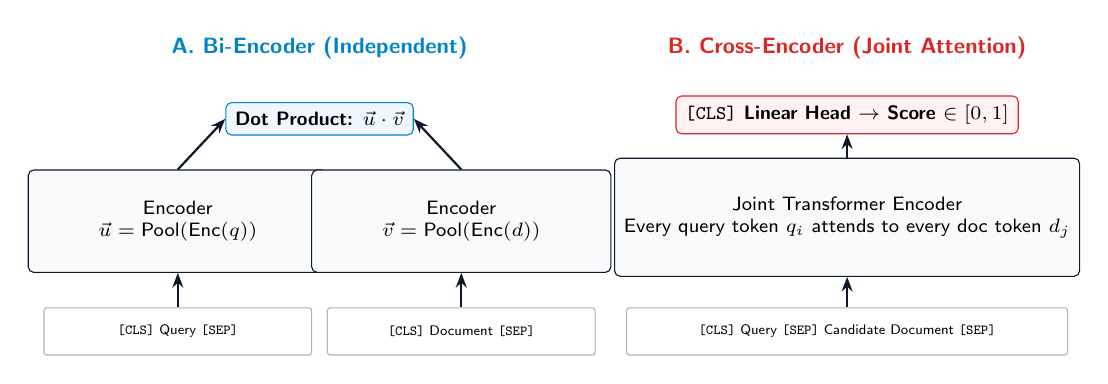
\begin{tikzpicture}[
  model/.style={draw=headingblue, fill=codebg, rounded corners=2pt, minimum width=3.8cm, minimum height=1.3cm, font=\sffamily\scriptsize, align=center},
  input/.style={draw=gray!60, fill=white, rounded corners=1pt, minimum width=3.4cm, minimum height=0.6cm, font=\sffamily\tiny, align=center},
  arrow/.style={-{Stealth[scale=0.8]}, thick, color=headingblue}
]

% Bi-Encoder
\node[font=\sffamily\bfseries\footnotesize, color=linkblue] at (2.0, 3.6) {A. Bi-Encoder (Independent)};
\node[input] (qin) at (0.2, 0) {\texttt{[CLS]} Query \texttt{[SEP]}};
\node[input] (din) at (3.8, 0) {\texttt{[CLS]} Document \texttt{[SEP]}};
\node[model] (encq) at (0.2, 1.4) {Encoder\\$\vec{u} = \text{Pool}(\text{Enc}(q))$};
\node[model] (encd) at (3.8, 1.4) {Encoder\\$\vec{v} = \text{Pool}(\text{Enc}(d))$};
\node[draw=linkblue, fill=exampleBg, rounded corners=2pt, font=\sffamily\scriptsize\bfseries] (dot) at (2.0, 2.7) {Dot Product: $\vec{u} \cdot \vec{v}$};

\draw[arrow] (qin) -- (encq);
\draw[arrow] (din) -- (encd);
\draw[arrow] (encq.north) -- (dot.west);
\draw[arrow] (encd.north) -- (dot.east);

% Cross-Encoder
\node[font=\sffamily\bfseries\footnotesize, color=warningRed] at (8.7, 3.6) {B. Cross-Encoder (Joint Attention)};
\node[input, minimum width=5.6cm] (crossin) at (8.7, 0) {\texttt{[CLS]} Query \texttt{[SEP]} Candidate Document \texttt{[SEP]}};
\node[model, minimum width=5.6cm, minimum height=1.5cm] (crossenc) at (8.7, 1.45) {
  Joint Transformer Encoder\\
  Every query token $q_i$ attends to every doc token $d_j$
};
\node[draw=warningRed, fill=warningBg, rounded corners=2pt, font=\sffamily\scriptsize\bfseries] (score) at (8.7, 2.75) {
  \texttt{[CLS]} Linear Head $\to$ Score $\in [0, 1]$
};

\draw[arrow] (crossin) -- (crossenc);
\draw[arrow] (crossenc) -- (score);

\end{tikzpicture}
\caption{Bi-Encoder vs Cross-Encoder: Bi-encoders pre-compute document vectors offline; cross-encoders run full token-level cross-attention jointly over each query-document pair.}
\label{fig:v2-ch03-bi-cross}
\end{figure}

\begin{itemize}[leftmargin=18pt]
  \item \textbf{Bi-Encoder}: Encodes query and document \emph{separately}. Because document vectors $\vec{v}$ are computed once at ingestion time, query latency is a single query forward pass plus vector lookup: 	extbf{$O(N \cdot D)$} for a flat scan or 	extbf{$O(\log N \cdot D)$} with an HNSW index (fast, $<5$ ms in RAM—not $O(1)$, since HNSW still scales logarithmically with $N$ and linearly with $D$). However, query tokens never directly inspect document tokens during encoding.
  \item \textbf{Cross-Encoder}: Concatenates \texttt{[CLS] query [SEP] document [SEP]} into one sequence. Every query token attends to every document token across $L$ layers ($O((|Q|+|D|)^2 \cdot L)$ per pair). It catches negations, exact clauses, and subtle modifiers that Bi-Encoders compress away—at the cost of 10--50 ms of GPU inference per batch of pairs.
\end{itemize}

\section{The Two-Stage Retrieval Cascade, HyDE, and MRR@K}

Because a Cross-Encoder cannot score 10 million documents in real time, production search uses a \textbf{two-stage cascade} (Figure~\ref{fig:v2-ch03-cascade}): Stage 1 uses fast Hybrid RRF (BM25 + Dense HNSW) to narrow 10M docs down to $\sim 50\text{--}100$ candidates in $<5$ ms; Stage 2 uses a Cross-Encoder to re-score only those top candidates in $\sim 25$ ms and keep the top 5 for the LLM.

\begin{figure}[htbp]
\centering
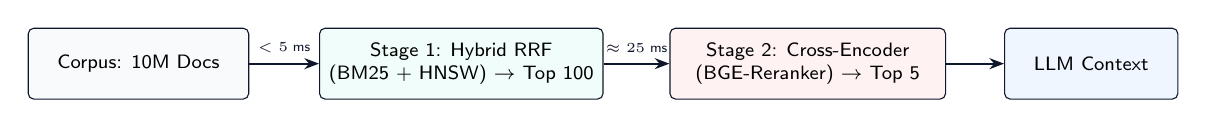
\begin{tikzpicture}[
  cascadestep/.style={draw=headingblue, fill=codebg, rounded corners=2pt, font=\sffamily\scriptsize, minimum height=0.9cm, align=center},
  arrow/.style={-{Stealth[scale=0.8]}, thick, color=headingblue}
]

\node[cascadestep, minimum width=2.8cm] (corpus) at (0, 0) {Corpus: 10M Docs};
\node[cascadestep, minimum width=3.6cm, fill=intuitionBg] (cands) at (4.1, 0) {Stage 1: Hybrid RRF\\(BM25 + HNSW) $\to$ Top 100};
\node[cascadestep, minimum width=3.5cm, fill=warningBg] (rerank) at (8.5, 0) {Stage 2: Cross-Encoder\\(BGE-Reranker) $\to$ Top 5};
\node[cascadestep, minimum width=2.2cm, fill=exampleBg] (llm) at (12.1, 0) {LLM Context};

\draw[arrow] (corpus) -- (cands) node[midway, above, font=\tiny\sffamily] {$<5$ ms};
\draw[arrow] (cands) -- (rerank) node[midway, above, font=\tiny\sffamily] {$\approx 25$ ms};
\draw[arrow] (rerank) -- (llm);

\end{tikzpicture}
\caption{Two-Stage Hybrid Retrieval Cascade: Fast recall in Stage 1 followed by high-precision cross-attention reranking in Stage 2.}
\label{fig:v2-ch03-cascade}
\end{figure}

Listing~\ref{lst:v2-ch03-cascade} shows the complete two-stage retriever. Notice that \texttt{retrieve} returns structured dictionaries matching its type annotation \texttt{list[dict[str, object]]}.

\begin{lstlisting}[language=Python, label={lst:v2-ch03-cascade}, caption={Two-Stage Hybrid Retrieval Cascade with Cross-Encoder Reranking}]
from sentence_transformers import CrossEncoder

class TwoStageRetriever:
    def __init__(
        self,
        bm25_index: ProductionBM25,
        vector_index,
        doc_store: dict[str, str],
        reranker_model: str = "BAAI/bge-reranker-large",
    ):
        self.bm25 = bm25_index
        self.vector_index = vector_index
        self.doc_store = doc_store
        self.reranker = CrossEncoder(reranker_model)

    def retrieve(self, query: str, top_k: int = 5) -> list[dict[str, object]]:
        # Stage 1: Fast candidate generation (100 lexical + 100 dense)
        sparse_hits = self.bm25.search(query, k=100)
        dense_hits = self.vector_index.search(query, k=100)

        fused = reciprocal_rank_fusion([sparse_hits, dense_hits], k=60)[:100]
        candidate_ids = [doc_id for doc_id, _ in fused]
        candidate_texts = [self.doc_store[did] for did in candidate_ids]
        if not candidate_texts:
            return []

        # Stage 2: Joint cross-encoder scoring
        pairs = [[query, text] for text in candidate_texts]
        scores = self.reranker.predict(pairs)

        ranked = sorted(
            zip(candidate_ids, candidate_texts, scores),
            key=lambda item: float(item[2]),
            reverse=True,
        )
        return [
            {"doc_id": did, "text": txt, "score": float(sc)}
            for did, txt, sc in ranked[:top_k]
        ]
\end{lstlisting}

\textbf{Step-by-Step Code Walkthrough:} On \texttt{query = "ALB-502 subnet 10.240.12.0/24"}:
\begin{enumerate}[leftmargin=18pt]
  \item Lines 18--19 fetch up to 100 exact-keyword \texttt{doc\_id}s via \texttt{self.bm25.search()} and 100 semantic \texttt{doc\_id}s via \texttt{self.vector\_index.search()}.
  \item Lines 21--23 merge both lists with \texttt{reciprocal\_rank\_fusion}, take the top 100 unique IDs, and fetch their text strings from \texttt{self.doc\_store}.
  \item Lines 28--29 pass all 100 \texttt{[query, text]} pairs in one GPU batch to \texttt{CrossEncoder.predict()}.
  \item Lines 31--39 sort descending by cross-encoder relevance logit and return the top 5 structured hit dictionaries.
\end{enumerate}

\subsection{Hypothetical Document Embeddings (HyDE)}
When user queries look nothing like formal manuals (e.g., \emph{``why do my ankles feel puffy when standing?''} vs clinical notes mentioning \emph{``bilateral peripheral edema''}), \textbf{HyDE} (Gao et al., 2022) prompts an LLM to draft a short hypothetical answer $\hat{D}$, embeds $\hat{D}$ instead of the raw question, and searches the vector index. Even if $\hat{D}$ guesses wrong specifics, its vocabulary and phrasing sit inside the target technical manifold.

\subsection{Measuring Rank Quality: Mean Reciprocal Rank (\texttt{MRR@K})}
To test whether hybrid fusion and reranking actually improve rank order, search engineers measure \textbf{Mean Reciprocal Rank at $K$ (\texttt{MRR@K})}. For each query $q \in \{1, \dots, Q\}$, find the rank $r_q \le K$ of the \emph{first} relevant document (if none appears in the top $K$, its reciprocal rank is $0$):
\begin{equation}
\text{MRR@K} = \frac{1}{|Q|} \sum_{q=1}^{|Q|} \frac{1}{r_q}
\end{equation}
For example, across 2 queries—if Query 1 finds its answer at rank 1 ($1/1 = 1.0$) and Query 2 finds its answer at rank 3 ($1/3 \approx 0.333$)—then $\text{MRR@10} = (1.0 + 0.333)/2 \approx 0.667$.

\begin{realworldbox}[Debugging SRE Post-Mortem Search Misses]
An internal incident-search service returned generic proxy docs for \emph{``ALB-502-BadGateway 10.240.12.0/24''}. Retrieval telemetry showed:
\begin{lstlisting}[basicstyle=\ttfamily\scriptsize]
dense_only_top3: ["http-502-guide"(0.84), "nginx-timeout"(0.81), "alb-intro"(0.79)]
bm25_top3:       ["inc-4412-subnet"(18.4), "vpc-cidr-map"(11.2), "http-502-guide"(6.1)]
hybrid_rrf_rerank_top1: "inc-4412-subnet" (cross_score=0.974)
\end{lstlisting}
Dense search fragmented \texttt{ALB-502-BadGateway} and \texttt{10.240.12.0/24} into subwords, ranking the real incident (\texttt{inc-4412-subnet}) at rank 47. Adding BM25 + RRF promoted \texttt{inc-4412-subnet} into the top 10, and the cross-encoder placed it at rank 1, raising team \texttt{MRR@10} from $0.41$ to $0.86$.
\end{realworldbox}

\begin{tryityourselfbox}[Computing Hybrid RRF + MRR@10 by Hand]
Suppose two test queries are run against a search index:
\begin{itemize}
  \item \textbf{Query 1} (answer is \texttt{doc\_X}): Dense ranks \texttt{[doc\_A, doc\_X, doc\_B]}; BM25 ranks \texttt{[doc\_X, doc\_C, doc\_A]}.
  \item \textbf{Query 2} (answer is \texttt{doc\_Y}): Dense ranks \texttt{[doc\_D, doc\_E, doc\_Y]}; BM25 misses \texttt{doc\_Y} entirely: \texttt{[doc\_D, doc\_F, doc\_G]}.
\end{itemize}
Compute the RRF ($k=60$) ranking for both queries, then calculate \texttt{MRR@10} for Dense alone vs Hybrid RRF. (Worked solution in Section~3.8.)
\end{tryityourselfbox}

\section{Chapter Summary \protect\& Key Takeaways}
\begin{itemize}[leftmargin=18pt]
  \item \textbf{Dense Limits}: Subword tokenization and latent compression erase exact error codes, SKUs, and CIDRs.
  \item \textbf{Okapi BM25}: Combines IDF rarity weighting, term-frequency saturation ($k_1$, asymptote $k_1+1$), and length normalization ($b$).
  \item \textbf{Reciprocal Rank Fusion}: Merges uncalibrated sparse and dense rankings via $\sum 1/(k + r_m(d))$ with $k \approx 60$.
  \item \textbf{Bi-Encoder vs Cross-Encoder}: Bi-encoders scale as $O(\log N \cdot D)$ via HNSW because document vectors are precomputed; cross-encoders run full token-to-token cross-attention ($O((|Q|+|D|)^2 L)$) on top candidates.
  \item \textbf{Two-Stage Cascade \& HyDE}: Generate $\sim 50\text{--}100$ candidates via Hybrid RRF, rerank with a Cross-Encoder, and evaluate rank quality with \texttt{MRR@K}.
\end{itemize}

\section{Exercises}

\subsection*{Mechanics}
\textbf{Exercise \thechapter.1}: Document $d_1$ ranks 2nd in BM25 and 14th in Dense search. Document $d_2$ ranks 6th in both systems. Compute the RRF scores of $d_1$ and $d_2$ with $k = 60$ and determine which ranks higher.

\textbf{Exercise \thechapter.2}: In the BM25 equation, prove what happens to document length $|D|$ when $b = 0$.

\subsection*{Debugging}
\textbf{Exercise \thechapter.3}: After adding a Cross-Encoder reranker, chatbot $p99$ latency jumps from 800 ms to 6.2 s. Profiling shows the reranker evaluates 500 candidate chunks of 512 tokens on every request. Propose two concrete changes to bring $p99$ under 1.2 s.

\subsection*{Architecture}
\textbf{Exercise \thechapter.4}: Design a multi-lingual e-commerce search engine spanning English, Japanese, and Arabic catalogs that supports cross-language queries while preserving exact SKU lookup accuracy.

\section{Detailed Solutions}

\subsection*{Solution \thechapter.1}
Using $\text{RRF}(d) = \frac{1}{60 + r_{\text{bm25}}} + \frac{1}{60 + r_{\text{dense}}}$:
\[
\text{RRF}(d_1) = \frac{1}{62} + \frac{1}{74} \approx 0.016129 + 0.013514 = 0.029643
\]
\[
\text{RRF}(d_2) = \frac{1}{66} + \frac{1}{66} = \frac{2}{66} \approx 0.030303
\]
Since $0.030303 > 0.029643$, $d_2$ outranks $d_1$ because RRF rewards balanced consensus across both retrievers.

\subsection*{Solution \thechapter.2}
In the denominator $f(q_i, D) + k_1 \cdot \left(1 - b + b \cdot \frac{|D|}{\text{avgdl}}\right)$, setting $b = 0$ gives:
\[
f(q_i, D) + k_1 \cdot (1 - 0 + 0) = f(q_i, D) + k_1
\]
The document length $|D|$ vanishes completely; length normalization is disabled.

\subsection*{Solution \thechapter.3}
1. \textbf{Shrink the Stage-1 candidate pool}: Passing 40--60 RRF candidates instead of 500 cuts cross-encoder compute by $\sim 90\%$ while retaining $>95\%$ of relevant hits. 2. \textbf{Distilled/Quantized Reranker}: Switch from a large 560M-parameter model to a distilled FP16/INT8 ONNX or TensorRT model (e.g., \texttt{bge-reranker-base} or \texttt{FlashRank}), cutting per-batch latency by 3--4$\times$.

\subsection*{Solution \thechapter.4}
1. \textbf{Language-specific BM25 analyzers}: Apply morphological tokenizers (e.g., Kuromoji for Japanese) alongside whitespace/Arabic normalizers in OpenSearch/Elasticsearch. 2. \textbf{Multilingual Bi-Encoder}: Use a shared-space multilingual embedding model (\texttt{multilingual-e5-large} or \texttt{text-embedding-3}). 3. \textbf{Exact SKU Regex Fast-Path}: Detect SKU patterns (e.g., \verb|^[A-Z]{2,5}-\d{3,}|) and route directly to an exact B-tree index lookup before hybrid fusion.

\subsection*{Solution (Try It Yourself)}
\textbf{Query 1}: \texttt{doc\_X} gets $\frac{1}{62} + \frac{1}{61} = 0.03252$ (rank 1); \texttt{doc\_A} gets $\frac{1}{61} + \frac{1}{63} = 0.03226$ (rank 2). \textbf{Query 2}: \texttt{doc\_D} gets $\frac{2}{61} = 0.03279$ (rank 1); \texttt{doc\_E}, \texttt{doc\_F} tie at $\frac{1}{62} = 0.01613$ (ranks 2--3); \texttt{doc\_Y} and \texttt{doc\_G} tie at $\frac{1}{63} = 0.01587$ (ranks 4--5).
\begin{itemize}
  \item \textbf{Dense alone}: Query 1 relevant at rank 2 ($1/2 = 0.50$); Query 2 relevant at rank 3 ($1/3 \approx 0.333$) $\implies \text{MRR@10} = (0.50 + 0.333)/2 = 0.417$.
  \item \textbf{Hybrid RRF}: Query 1 relevant at rank 1 ($1.0$); Query 2 relevant at rank 4 or 5 ($\approx 0.20$--$0.25$) $\implies \text{MRR@10} \approx (1.0 + 0.22)/2 = 0.61$.
\end{itemize}

\begin{labbridgebox}[Hands-On Exercises \& Project Bridge]
Implement BM25 and RRF directly in \texttt{exercises/volume2/ex02\_bm25\_tf\_idf\_search.py} and \texttt{exercises/volume2/ex03\_reciprocal\_rank\_fusion.py}, then run the full two-stage cascade in \texttt{projects/p06-rag-hybrid-rerank/} (\texttt{rag/dense.py}, \texttt{rag/sparse.py}, \texttt{rag/fusion.py}, \texttt{rag/reranker.py}, \texttt{rag/pipeline.py}, tested via \texttt{tests/test\_hybrid\_rag.py}).
\end{labbridgebox}

\section{Further Reading \protect\& Citations}
\begin{itemize}[leftmargin=18pt]
  \item Robertson, S., \& Zaragoza, H. (2009). \emph{The Probabilistic Relevance Framework: BM25 and Beyond}. Foundations and Trends in Information Retrieval, 3(4), 333--389.
  \item Cormack, G. V., Clarke, C. L., \& Büttcher, S. (2009). \emph{Reciprocal Rank Fusion Outperforms Condorcet and Individual Rank Learning Methods}. ACM SIGIR.
  \item Gao, L., et al. (2022). \emph{Precise Zero-Shot Dense Retrieval without Relevance Labels (HyDE)}. arXiv:2212.10496.
\end{itemize}

\chapter{Agent Architectures and Orchestration: ReAct, Planning, and Multi-Agent Systems}
\label{chap:agents}

\begin{chaptergoalsbox}
\textbf{What You Will Learn:}
\begin{itemize}[leftmargin=15pt]
  \item Cognitive agent patterns starting from a concrete multi-turn ReAct trace: ReAct, Plan-and-Solve, and Reflexion.
  \item Tool-calling wire protocols: JSON Schema (Draft 2020-12), Pydantic validation, and exception feedback loops.
  \item Deterministic execution guards: canonical JSON loop detection, step/token ceilings, and output truncation.
  \item Expression sandboxing with Python's Abstract Syntax Tree (\texttt{ast}) and why \texttt{eval()} is never safe.
  \item Multi-agent topologies: Supervisor-Worker context isolation and peer-review validation.
\end{itemize}

\textbf{What You Should Already Understand:}
\begin{itemize}[leftmargin=15pt]
  \item Python functions, dictionaries, exceptions, and JSON strings.
  \item Basic HTTP request/response concepts and status codes.
\end{itemize}

\textbf{Why This Topic Exists:}
A standalone LLM prompt can draft text, but it cannot check a database, inspect pod logs, or open a pull request. Turning an LLM into an \textbf{agent} means wiring it into a loop where it calls external tools and reacts to real outputs. Without strict input validation, loop detection, sandboxing, and token budgets, autonomous agents hallucinate arguments, spin in infinite retry loops, or execute unsafe expressions.

\textbf{Motivating Practical Problem:}
A DevOps remediation agent is asked to diagnose a crashing Kubernetes service. It must inspect pod logs, confirm an Out-Of-Memory (OOM) exit code, read current Helm memory limits, propose a safe memory bump, and recover gracefully if the metrics API times out---all without burning \$500 in an accidental retry loop.
\end{chaptergoalsbox}

\section{Inside a Real ReAct Trace: Reason + Act}

An AI \textbf{agent} is a loop that lets an LLM perceive its environment through \emph{tool outputs} and act upon that environment through \emph{tool calls}. Earlier prompt techniques either reasoned in isolation (Chain-of-Thought, which invents fake facts if it lacks live data) or fired tools blindly without checking intermediate errors.

\textbf{ReAct} (Yao et al., 2022) interleaves internal reasoning (\textbf{Thought}), external invocation (\textbf{Action}), and real tool feedback (\textbf{Observation}):
\begin{equation}
\text{Thought}_t \longrightarrow \text{Action}_t \longrightarrow \text{Observation}_t \longrightarrow \text{Thought}_{t+1} \longrightarrow \dots
\end{equation}

Before inspecting any code, read an actual 3-turn ReAct transcript for our crashing Kubernetes service:
\begin{quote}\small
\textbf{User:} Why is \texttt{payments-api} restarting in \texttt{prod}, and how should we fix it?\\[4pt]
\textbf{Thought 1:} I should inspect the pod termination status and recent logs in namespace \texttt{prod}.\\
\textbf{Action 1:} \texttt{get\_pod\_status(namespace="prod", pod\_prefix="payments-api")}\\
\textbf{Observation 1:} \texttt{\{"pod": "payments-api-7f9b", "restarts": 14, "last\_exit\_code": 137, "reason": "OOMKilled"\}}\\[4pt]
\textbf{Thought 2:} Exit code 137 means the Linux kernel killed the container for exceeding its memory limit. I need to check the current Helm memory limit before suggesting a bump.\\
\textbf{Action 2:} \texttt{read\_helm\_values(service="payments-api", key="resources.limits.memory")}\\
\textbf{Observation 2:} \texttt{\{"resources.limits.memory": "512Mi", "peak\_observed\_rss": "508Mi"\}}\\[4pt]
\textbf{Thought 3:} The service hit its 512Mi ceiling. Doubling the limit to 1024Mi provides headroom. No further tool calls are needed.\\
\textbf{Final Answer:} \texttt{payments-api} is being \texttt{OOMKilled} (exit code 137) against a 512Mi limit. Recommend raising \texttt{resources.limits.memory} to \texttt{1024Mi}.
\end{quote}

Figure~\ref{fig:v2-ch04-react} shows this cyclic flow. Each \textbf{Observation} anchors the next \textbf{Thought} in ground-truth system state rather than guesswork.

\begin{figure}[htbp]
\centering
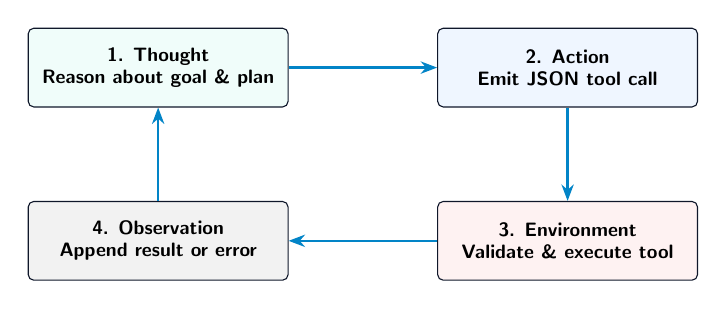
\begin{tikzpicture}[
  node/.style={draw=headingblue, fill=codebg, rounded corners=2pt, font=\sffamily\scriptsize\bfseries, minimum width=3.3cm, minimum height=1.0cm, align=center},
  arrow/.style={-{Stealth[scale=0.9]}, thick, color=linkblue}
]

\node[node, fill=intuitionBg] (thought) at (0, 2) {1. Thought\\Reason about goal \& plan};
\node[node, fill=exampleBg] (action) at (5.2, 2) {2. Action\\Emit JSON tool call};
\node[node, fill=warningBg] (env) at (5.2, -0.2) {3. Environment\\Validate \& execute tool};
\node[node, fill=gray!10] (obs) at (0, -0.2) {4. Observation\\Append result or error};

\draw[arrow] (thought) -- (action);
\draw[arrow] (action) -- (env);
\draw[arrow] (env) -- (obs);
\draw[arrow] (obs) -- (thought);

\end{tikzpicture}
\caption{The Cyclic ReAct (Reason + Act) Execution Loop.}
\label{fig:v2-ch04-react}
\end{figure}

\subsection{Plan-and-Solve and Reflexion}
ReAct is flexible, but over 15--20 steps an agent can suffer \emph{myopic drift}—forgetting its original objective while chasing a side error. Two complementary patterns address this:
\begin{itemize}[leftmargin=18pt]
  \item \textbf{Plan-and-Solve} (Wang et al., 2023): Splits work into a \textbf{Planner} (which writes a numbered task DAG upfront) and an \textbf{Executor} (which completes each sub-task in order and re-plans only if an assumption breaks).
  \item \textbf{Reflexion} (Shinn et al., 2023): When an attempt fails a test or API check (Figure~\ref{fig:v2-ch04-reflexion}), a separate reflection step writes a brief post-mortem into an episodic memory buffer (e.g., \emph{``I passed an ISO date string instead of an integer UNIX timestamp''}) so the next trial avoids repeating the same mistake.
\end{itemize}

\begin{figure}[htbp]
\centering
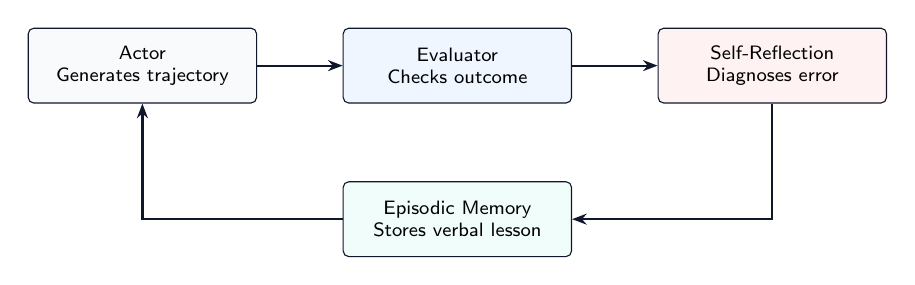
\begin{tikzpicture}[
  box/.style={draw=headingblue, fill=codebg, rounded corners=2pt, font=\sffamily\scriptsize, minimum width=2.9cm, minimum height=0.95cm, align=center},
  arrow/.style={-{Stealth[scale=0.8]}, thick, color=headingblue}
]

\node[box] (actor) at (0, 1.5) {Actor\\Generates trajectory};
\node[box, fill=exampleBg] (eval) at (4.0, 1.5) {Evaluator\\Checks outcome};
\node[box, fill=warningBg] (self) at (8.0, 1.5) {Self-Reflection\\Diagnoses error};
\node[box, fill=intuitionBg] (mem) at (4.0, -0.45) {Episodic Memory\\Stores verbal lesson};

\draw[arrow] (actor) -- (eval);
\draw[arrow] (eval) -- (self);
\draw[arrow] (self) |- (mem);
\draw[arrow] (mem) -| (actor);

\end{tikzpicture}
\caption{Reflexion Architecture: Failed executions trigger verbal self-critiques stored in short-term episodic memory.}
\label{fig:v2-ch04-reflexion}
\end{figure}

\section{Tool Calling Protocols and Validation Self-Correction}

How does an LLM know what arguments a Python tool expects? A \textbf{JSON Schema} is a standard JSON document describing an object's allowed field names, types (\texttt{"string"}, \texttt{"integer"}), bounds (\texttt{minimum}, \texttt{maximum}), and \texttt{required} keys. Rather than hand-writing schemas, Pydantic v2 generates them automatically via \texttt{model\_json\_schema()}, which conforms to \textbf{JSON Schema Draft 2020-12} (Listing~\ref{lst:v2-ch04-schema}).

\begin{lstlisting}[language=Python, label={lst:v2-ch04-schema}, caption={Declaring Tool Schemas with Pydantic v2 (JSON Schema Draft 2020-12)}]
from pydantic import BaseModel, Field

class RestartPodInput(BaseModel):
    namespace: str = Field(
        ...,
        description="Kubernetes namespace containing the target pod, e.g. 'prod'."
    )
    pod_name: str = Field(
        ...,
        description="Exact pod name to restart."
    )
    grace_period_seconds: int = Field(
        default=30, ge=0, le=300,
        description="Grace period in seconds (0..300) before SIGKILL."
    )
    force: bool = Field(
        default=False,
        description="Set true only if graceful deletion stalls."
    )

# Pydantic v2 model_json_schema() emits JSON Schema Draft 2020-12
tool_definition = {
    "type": "function",
    "function": {
        "name": "restart_kubernetes_pod",
        "description": "Restarts a pod by issuing a Kubernetes delete call.",
        "parameters": RestartPodInput.model_json_schema()
    }
}
\end{lstlisting}

When the model decides to call \texttt{restart\_kubernetes\_pod}, the API returns a \texttt{tool\_call} object carrying \texttt{name} and a raw JSON string \texttt{arguments}. Never pass raw parsed JSON straight to an internal handler—validate it first (Listing~\ref{lst:v2-ch04-dispatch}). Note that \texttt{async def} / \texttt{await} allows our dispatcher to run I/O-bound tool calls concurrently on Python's event loop without blocking other requests.

\begin{lstlisting}[language=Python, label={lst:v2-ch04-dispatch}, caption={Safe Tool Dispatch and Schema Validation Loop}]
import json
from pydantic import ValidationError

async def dispatch_tool_call(tool_call, registered_tools: dict) -> dict:
    func_name = tool_call.name
    raw_args = tool_call.arguments

    if func_name not in registered_tools:
        return {
            "is_error": True,
            "error": f"Unknown tool '{func_name}'. Available: {list(registered_tools.keys())}"
        }

    tool_meta = registered_tools[func_name]
    schema_model = tool_meta["schema"]
    callable_func = tool_meta["handler"]

    # 1. Parse JSON string safely
    try:
        args_dict = json.loads(raw_args) if isinstance(raw_args, str) else raw_args
    except json.JSONDecodeError as e:
        return {"is_error": True, "error": f"Invalid JSON syntax: {e}"}

    # 2. Validate types and constraints against Pydantic schema
    try:
        validated_args = schema_model(**args_dict)
    except ValidationError as ve:
        return {
            "is_error": True,
            "error": f"Parameter validation failed: {ve.json()}. Fix arguments."
        }

    # 3. Execute tool and catch runtime exceptions as Observations
    try:
        result = await callable_func(validated_args)
        return {"is_error": False, "result": result}
    except Exception as exc:
        return {
            "is_error": True,
            "error": f"Execution error in '{func_name}': {type(exc).__name__}: {exc}"
        }
\end{lstlisting}

\begin{intuitionbox}[Tracing One Self-Correction Iteration on \texttt{ValidationError}]
Suppose the LLM emits an out-of-range argument:
\begin{center}\small\ttfamily
tool\_call(id="call\_91", name="restart\_kubernetes\_pod", arguments='\{"namespace":"prod","pod\_name":"payments-api-7f9b","grace\_period\_seconds":900\}')
\end{center}
\begin{enumerate}
  \item Line 20 parses the JSON cleanly into a Python \texttt{dict}.
  \item Line 26 runs \texttt{RestartPodInput(**args\_dict)}, which raises \texttt{ValidationError}: \texttt{grace\_period\_seconds: Input should be less than or equal to 300}.
  \item Instead of crashing, lines 28--31 return \texttt{\{"is\_error": True, "error": "Parameter validation failed: ..."\}}.
  \item The agent loop appends a \texttt{tool} message tagged with \texttt{tool\_call\_id="call\_91"} containing that error. On the next turn, the LLM reads the \texttt{<= 300} constraint and re-emits \texttt{"grace\_period\_seconds": 120}, which passes validation and executes!
\end{enumerate}
\end{intuitionbox}

\section{Deterministic Runtimes and Canonical Loop Detection}

An unguarded \texttt{while} loop around an LLM can burn thousands of dollars in minutes if a tool keeps failing or returning 20,000-character logs. Production runtimes enforce three tripwires (Listing~\ref{lst:v2-ch04-loop}):
\begin{enumerate}[leftmargin=18pt]
  \item \textbf{Canonical Loop Detection}: If an LLM invokes \texttt{search(\{"a": 1, "b": 2\})} and then \texttt{search(\{"b": 2, "a": 1\})} with whitespace or key order changed, naive string comparison misses the duplicate! Normalizing arguments via \texttt{json.dumps(parsed, sort\_keys=True, separators=(",", ":"))} ensures identical calls always produce the exact same signature.
  \item \textbf{Step \& Token Budgets}: Cap both reasoning turns (\texttt{max\_steps}) and cumulative tokens (\texttt{max\_tokens}).
  \item \textbf{Observation Truncation}: Truncate oversized tool outputs before appending them to conversation history.
\end{enumerate}

\begin{lstlisting}[language=Python, label={lst:v2-ch04-loop}, caption={Production Execution Loop with Canonical Loop Detection and Tripwires}]
import json

def _canonical_call_sig(name: str, raw_args: str | dict) -> tuple[str, str]:
    try:
        parsed = json.loads(raw_args) if isinstance(raw_args, str) else raw_args
        return (name, json.dumps(parsed, sort_keys=True, separators=(",", ":")))
    except (json.JSONDecodeError, TypeError):
        return (name, str(raw_args))

class ProductionAgentLoop:
    def __init__(self, llm_client, tools: dict, max_steps: int = 10, max_tokens: int = 15000):
        self.llm = llm_client
        self.tools = tools
        self.max_steps = max_steps
        self.max_tokens = max_tokens

    async def run(self, user_prompt: str) -> str:
        messages = [{"role": "user", "content": user_prompt}]
        total_tokens_consumed = 0
        call_history: list[tuple[str, str]] = []

        for step_count in range(1, self.max_steps + 1):
            response = await self.llm.invoke(messages, tools=list(self.tools.values()))
            total_tokens_consumed += response.usage.total_tokens
            if total_tokens_consumed > self.max_tokens:
                raise RuntimeError("Token budget exceeded safety limit. Aborting.")

            messages.append(response.message)
            if not response.tool_calls:
                return response.content

            for tool_call in response.tool_calls:
                call_sig = _canonical_call_sig(tool_call.name, tool_call.arguments)
                if call_history.count(call_sig) >= 2:
                    tool_result = {
                        "is_error": True,
                        "error": "CRITICAL: Identical tool call repeated twice. Change strategy."
                    }
                else:
                    call_history.append(call_sig)
                    tool_result = await dispatch_tool_call(tool_call, self.tools)

                str_res = str(
                    tool_result["result"] if not tool_result["is_error"] else tool_result["error"]
                )
                if len(str_res) > 2000:
                    str_res = str_res[:2000] + "... [TRUNCATED]"

                messages.append({
                    "role": "tool",
                    "tool_call_id": tool_call.id,
                    "content": str_res
                })

        return "Task could not be completed within maximum allowed reasoning steps."
\end{lstlisting}

\section{Safe Tool Execution: \texttt{ast} Expression Sandboxing}

Suppose an LLM needs a calculator tool to compute \texttt{"2 + 3 * 4"}. The worst mistake in Python is calling \texttt{eval(expression)}: if a prompt-injected document tricks the model into sending \texttt{"\_\_import\_\_('os').system('id')"}, \texttt{eval()} executes arbitrary shell commands on your server! Regex blocklists also fail because Python offers dozens of sneaky attribute-lookup tricks.

The safe engineering solution uses Python's \textbf{Abstract Syntax Tree (\texttt{ast})} module. How does Python turn source text into execution, and why does stopping at the AST keep us safe?
\begin{enumerate}[leftmargin=18pt]
  \item \textbf{Tokenization}: The lexer breaks raw characters \texttt{"2 + 3 * 4"} into tokens (\texttt{2}, \texttt{+}, \texttt{3}, \texttt{*}, \texttt{4}).
  \item \textbf{Parsing into an AST}: \texttt{ast.parse(expr, mode="eval")} builds an inert tree of syntax nodes honoring operator precedence—\emph{without executing anything}:
  \[
  \texttt{Expression(BinOp(left=Constant(2), op=Add(), right=BinOp(Constant(3), Mult(), Constant(4))))}
  \]
  \item \textbf{Whitelisted Tree Evaluation}: Our code walks the tree recursively and allows \emph{only} numeric constants and safe arithmetic operators (\texttt{Add}, \texttt{Sub}, \texttt{Mult}, \texttt{Div}, \texttt{Pow} with bounded exponents).
\end{enumerate}
If an attacker sends \texttt{"\_\_import\_\_('os').system('id')"}, \texttt{ast.parse} builds a \texttt{Call} node; our evaluator sees \texttt{Call} is not in the whitelist and immediately raises \texttt{ValueError("Unsupported AST node: Call")} before a single function is ever invoked!

\section{Multi-Agent Topologies: Supervisor-Worker Isolation}

When a single agent manages 15 tools and reads huge logs, its prompt fills with noisy intermediate traces. \textbf{Supervisor-Worker} architectures (Figure~\ref{fig:v2-ch04-supervisor}) split work across specialized sub-agents.

\begin{figure}[htbp]
\centering
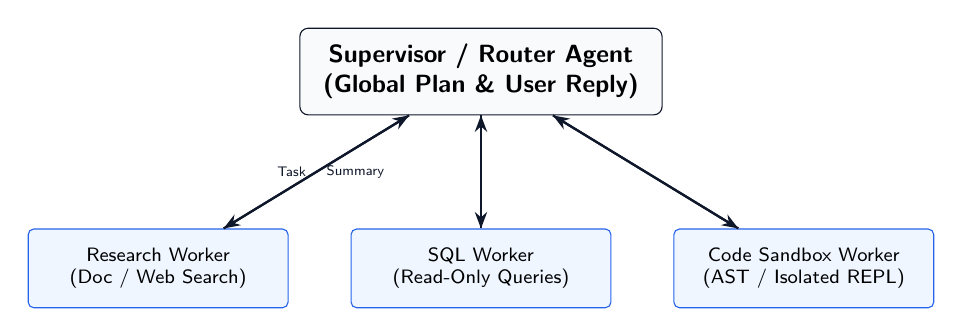
\begin{tikzpicture}[
  supervisor/.style={draw=headingblue, fill=codebg, rounded corners=3pt, font=\sffamily\small\bfseries, minimum width=4.6cm, minimum height=1.1cm, align=center},
  worker/.style={draw=exampleBlue, fill=exampleBg, rounded corners=2pt, font=\sffamily\scriptsize, minimum width=3.3cm, minimum height=1.0cm, align=center},
  arrow/.style={-{Stealth[scale=0.9]}, thick, color=headingblue}
]

\node[supervisor] (sup) at (0, 2.5) {Supervisor / Router Agent\\(Global Plan \& User Reply)};
\node[worker] (w1) at (-4.1, 0) {Research Worker\\(Doc / Web Search)};
\node[worker] (w2) at (0, 0) {SQL Worker\\(Read-Only Queries)};
\node[worker] (w3) at (4.1, 0) {Code Sandbox Worker\\(AST / Isolated REPL)};

\draw[arrow] (sup) -- (w1) node[midway, left, font=\tiny\sffamily] {Task};
\draw[arrow] (w1) -- (sup) node[midway, right, font=\tiny\sffamily] {Summary};
\draw[arrow] (sup) -- (w2);
\draw[arrow] (w2) -- (sup);
\draw[arrow] (sup) -- (w3);
\draw[arrow] (w3) -- (sup);

\end{tikzpicture}
\caption{Supervisor-Worker Topology: Workers run in isolated context windows and return compact summaries to the Supervisor.}
\label{fig:v2-ch04-supervisor}
\end{figure}

\begin{underthehoodbox}[Context Isolation as the Primary Payoff]
Suppose the SQL Worker runs 12 exploratory schema queries generating 8,000 tokens of column dumps and failed SQL syntax corrections. Because the SQL Worker runs inside its own private message list, it returns only a 150-token summary to the Supervisor. The Supervisor's prompt stays clean, avoiding both token bloat and ``Lost in the Middle'' attention degradation.
\end{underthehoodbox}

\begin{realworldbox}[Multi-Agent Security Review \& Canonical Loop Incident]
A platform team deployed two patterns: (1) a Terraform Coder + Security Auditor pair, and (2) an incident triage agent. During IaC review, the Coder drafted an S3 bucket without public access blocks; the Auditor flagged \texttt{CIS-AWS-2.1.4} (S3 Block Public Access), prompting an automatic patch before any PR was opened. Meanwhile, the triage agent produced an unexpected \$420 overnight bill:
\begin{lstlisting}[basicstyle=\ttfamily\scriptsize]
step=3  tool=query_metrics args='{"service":"auth","window":"5m"}'
step=4  tool=query_metrics args='{"window":"5m","service":"auth"}'  # bypassed string check!
step=5  tool=query_metrics args='{"service": "auth", "window": "5m"}'
\end{lstlisting}
Because the old loop detector compared raw unparsed argument strings, flipped JSON key ordering bypassed loop detection. Switching to \texttt{\_canonical\_call\_sig} (Listing~\ref{lst:v2-ch04-loop}) caught the duplicate on step 5 and halted the spin.
\end{realworldbox}

\begin{tryityourselfbox}[Build a Safe AST Calculator Tool]
Build a tool \texttt{safe\_calculate} that evaluates mathematical expressions sent by an LLM:
\begin{enumerate}
  \item Define a Pydantic model \texttt{MathExpression} with field \texttt{expression: str}.
  \item Parse with \texttt{ast.parse(expr, mode="eval")} and evaluate \emph{only} numeric constants, unary negation (\texttt{USub}), and binary operators (\texttt{Add, Sub, Mult, Div, Pow} with bounded exponent \texttt{<= 100}).
  \item Verify that \texttt{"2 + 3 * 4"} returns \texttt{14.0} while \texttt{"\_\_import\_\_('os').system('id')"} fails safely with an error JSON object.
\end{enumerate}
(Complete worked solution in Section~4.9.)
\end{tryityourselfbox}

\section{Chapter Summary \protect\& Key Takeaways}
\begin{itemize}[leftmargin=18pt]
  \item \textbf{Cognitive Loops}: ReAct grounds reasoning in tool Observations; Plan-and-Solve curbs multi-step drift; Reflexion stores verbal failure lessons.
  \item \textbf{Validation \& Recovery}: Pydantic v2 emits JSON Schema Draft 2020-12; serializing \texttt{ValidationError} back as a \texttt{tool} message lets frontier LLMs self-correct invalid arguments.
  \item \textbf{Deterministic Guards}: Canonicalize JSON arguments before counting repeats, cap steps and tokens, and truncate huge tool outputs.
  \item \textbf{AST Sandboxing}: Never run \texttt{eval()} on LLM strings; parse to an AST and evaluate only whitelisted arithmetic nodes.
  \item \textbf{Context Isolation}: Supervisor-Worker systems keep messy intermediate tool traces out of the main orchestrator's prompt.
\end{itemize}

\section{Exercises}

\subsection*{Mechanics}
\textbf{Exercise \thechapter.1}: Write the JSON Schema Draft 2020-12 tool definition for:
\begin{lstlisting}[language=Python]
def transfer_funds(
    source_account: str, destination_account: str, amount_cents: int, currency: str = "USD"
) -> bool:
    """Transfers funds between corporate ledger accounts."""
\end{lstlisting}

\textbf{Exercise \thechapter.2}: In step 1 of a ReAct loop, the LLM calls \texttt{search\_database("user\_id=12")} with \texttt{id="call\_abc123"}. The database returns \texttt{InvalidColumnError: Table 'users' has no column 'user\_id'}. Write the exact \texttt{tool} message dictionary appended to \texttt{messages} so the LLM can self-correct.

\subsection*{Debugging}
\textbf{Exercise \thechapter.3}: Two Slack support bots talk to each other overnight and burn \$4,000 in API fees repeating \emph{``Thank you, let me know if you need anything else!''}. Identify two missing termination guards and write the Python check to stop the loop.

\subsection*{Architecture}
\textbf{Exercise \thechapter.4}: Design a customer-service multi-agent system for an airline with a Triage Supervisor, Flight Booking Worker, Baggage Tracking Worker, and Compensation Claims Worker. Specify state isolation, authentication gating, and human-approval thresholds.

\section{Detailed Solutions}

\subsection*{Solution \thechapter.1}
\begin{lstlisting}[language=Python]
tool_schema = {
    "type": "function",
    "function": {
        "name": "transfer_funds",
        "description": "Transfers funds between corporate ledger accounts.",
        "parameters": {
            "type": "object",
            "properties": {
                "source_account": {"type": "string", "description": "Source ledger ID."},
                "destination_account": {"type": "string", "description": "Target ledger ID."},
                "amount_cents": {"type": "integer", "minimum": 1, "description": "Cents to transfer."},
                "currency": {"type": "string", "enum": ["USD", "EUR", "GBP"], "default": "USD"}
            },
            "required": ["source_account", "destination_account", "amount_cents"]
        }
    }
}
\end{lstlisting}

\subsection*{Solution \thechapter.2}
\begin{lstlisting}[language=Python]
tool_message = {
    "role": "tool",
    "tool_call_id": "call_abc123",
    "name": "search_database",
    "content": json.dumps({
        "status": "error",
        "error_type": "InvalidColumnError",
        "message": "Table 'users' has no column 'user_id'. Available: ['id', 'email', 'created_at']"
    })
}
\end{lstlisting}

\subsection*{Solution \thechapter.3}
The bot lacked: (1) a monotonic turn counter across agent-to-agent replies, and (2) an explicit termination sentinel such as \texttt{[TASK\_COMPLETE]} in the system prompt. Fix:
\begin{lstlisting}[language=Python]
if "[TASK_COMPLETE]" in response.content or step_count >= 6:
    return response.content.replace("[TASK_COMPLETE]", "").strip()
\end{lstlisting}

\subsection*{Solution \thechapter.4}
1. \textbf{Shared State \& Isolation}: Store only \texttt{user\_id}, \texttt{verified\_identity: bool}, \texttt{pnr}, and \texttt{messages} in shared orchestrator state; keep worker SQL/API scratchpads private inside each worker context. 2. \textbf{Auth Gate}: Before routing to Booking or Compensation workers, verify \texttt{verified\_identity == True}; otherwise route to an identity-verification node. 3. \textbf{Human Escalation Gate}: Any payout exceeding \$200 pauses via an explicit interrupt (Chapter~5) for human sign-off.

\subsection*{Solution (Try It Yourself)}
\begin{lstlisting}[language=Python]
import ast, json, operator
from pydantic import BaseModel

class MathExpression(BaseModel):
    expression: str

OPS = {ast.Add: operator.add, ast.Sub: operator.sub,
       ast.Mult: operator.mul, ast.Div: operator.truediv, ast.Pow: operator.pow}

def safe_calculate(payload: MathExpression) -> str:
    def _eval(node: ast.AST) -> float:
        if isinstance(node, ast.Expression):
            return _eval(node.body)
        if isinstance(node, ast.Constant) and isinstance(node.value, (int, float)):
            return float(node.value)
        if isinstance(node, ast.UnaryOp) and isinstance(node.op, ast.USub):
            return -_eval(node.operand)
        if isinstance(node, ast.BinOp) and type(node.op) in OPS:
            left, right = _eval(node.left), _eval(node.right)
            if isinstance(node.op, ast.Pow) and abs(right) > 100:
                raise ValueError("Exponent exceeds safety cap of 100.")
            return float(OPS[type(node.op)](left, right))
        raise ValueError(f"Unsupported AST node: {type(node).__name__}")
    try:
        tree = ast.parse(payload.expression, mode="eval")
        return json.dumps({"ok": True, "result": _eval(tree)})
    except Exception as exc:
        return json.dumps({"ok": False, "error": str(exc)})
\end{lstlisting}

\begin{labbridgebox}[Project Bridge]
Inspect how read-only tools and privileged side-effect tools are separated and dispatched in \texttt{projects/p05-langgraph-agent-state/agent/tools.py} and \texttt{projects/p05-langgraph-agent-state/agent/research\_agent.py}.
\end{labbridgebox}

\section{Further Reading \protect\& Citations}
\begin{itemize}[leftmargin=18pt]
  \item Yao, S., et al. (2022). \emph{ReAct: Synergizing Reasoning and Acting in Language Models}. ICLR.
  \item Wang, L., et al. (2023). \emph{Plan-and-Solve Prompting}. ACL.
  \item Shinn, N., et al. (2023). \emph{Reflexion: Language Agents with Verbal Reinforcement Learning}. NeurIPS.
\end{itemize}

\chapter{LangGraph and Stateful Agent Architectures}
\label{chap:langgraph}

\begin{chaptergoalsbox}
\textbf{What You Will Learn:}
\begin{itemize}[leftmargin=15pt]
  \item Why in-memory agent loops fail across crashes or human approvals, and how state machines solve durability.
  \item Channel reducers and monoids in plain English before Bulk Synchronous Parallel (Pregel) supersteps.
  \item Constructing cyclic \texttt{StateGraph} workflows and tracing state across Supersteps 0, 1, and 2.
  \item Production persistence: PostgreSQL \texttt{AsyncPostgresSaver} schema (\texttt{checkpoints}, \texttt{checkpoint\_blobs}, \texttt{checkpoint\_writes}) and \texttt{AsyncConnectionPool(open=False)}.
  \item Human-in-the-loop (HITL) interrupts: \texttt{interrupt\_before} vs \texttt{langgraph.types.interrupt()}, and time-travel debugging.
\end{itemize}

\textbf{What You Should Already Understand:}
\begin{itemize}[leftmargin=15pt]
  \item Tool-calling ReAct loops and Pydantic schemas (Chapter~4).
  \item Python dictionaries, \texttt{TypedDict}, and basic SQL primary/foreign keys.
\end{itemize}

\textbf{Why This Topic Exists:}
Chapter~4's \texttt{ProductionAgentLoop} works well for a 10-second task inside one Python process. However, if the container restarts at step 4—or if a financial transaction needs a compliance officer to click ``Approve'' three hours later—an in-memory \texttt{while} loop loses all progress. Production agents need explicit, serializable state transitions stored in a database after every step.

\textbf{Motivating Practical Problem:}
A financial reconciliation agent parses corporate invoices, cross-checks an ERP ledger, and—whenever a discrepancy exceeds \$10,000—must pause for a compliance officer's approval before posting ledger adjustments. If the worker crashes mid-audit, it must resume from the exact checkpoint without re-charging APIs or duplicating ledger entries.
\end{chaptergoalsbox}

\section{Why Single Loops Break Across Process Boundaries}

Early LLM frameworks modeled workflows as linear pipelines:
\begin{equation}
\text{Input} \longrightarrow \text{Prompt} \longrightarrow \text{LLM} \longrightarrow \text{Parser} \longrightarrow \text{Result}
\end{equation}
Linear pipelines cannot loop back when a tool fails, cannot branch cleanly across parallel workers, and cannot pause for hours while a human reviews a draft. LangGraph reformulates agent orchestration as a \textbf{state machine} inspired by Google's \textbf{Pregel} graph engine (Malewicz et al., 2010).

\begin{intuitionbox}[The Rail Network Metaphor]
A linear chain is a train on one track: if a signal turns red, the whole trip stalls or derails. A stateful graph is a rail network with switches (\textbf{conditional edges}), sidings (\textbf{tool loops}), and a shared cargo manifest (\textbf{State}). At every station (\textbf{node}), workers inspect the manifest, emit cargo updates (\textbf{deltas}), and pause cleanly at red signals (\textbf{interrupts}) while the manifest sits safely locked in a database vault.
\end{intuitionbox}

\section{Reducers and Monoids in Plain English}

Suppose two parallel workers inspect different invoices at the exact same moment. Worker A finds discrepancy \texttt{"ERR-101"}, and Worker B finds \texttt{"ERR-102"}. If both run \texttt{state["discrepancies"] = [found\_item]}, Worker B overwrites Worker A's finding! Even \texttt{list.append()} across concurrent tasks can interleave unpredictably.

Instead of letting nodes mutate shared state directly, LangGraph makes every node return a \emph{partial update} (a \textbf{delta}) and delegates merging to a \textbf{channel reducer}:
\begin{itemize}[leftmargin=18pt]
  \item \textbf{Reducer}: Simply a two-argument merge function \texttt{combine(existing\_value, incoming\_delta) -> new\_value}. For example, \texttt{operator.add([A], [B])} returns \texttt{[A, B]}.
  \item \textbf{Monoid}: A reducer that also obeys two clean rules: (1) \textbf{associativity}—grouping doesn't change the outcome, so $(S \oplus \Delta_A) \oplus \Delta_B = S \oplus (\Delta_A \oplus \Delta_B)$; and (2) an \textbf{identity value} (such as \texttt{[]} for lists or \texttt{0} for addition) that leaves state unchanged when merged.
\end{itemize}
Why does this matter in production? Because when two parallel nodes finish in unpredictable order, an associative reducer at the synchronization point combines their deltas deterministically with zero race conditions.

\section{The Pregel Superstep Model and State Trace}

In Pregel, execution advances in discrete rounds called \textbf{Supersteps} (Figure~\ref{fig:v2-ch05-pregel}). Every superstep has three strict phases:
\begin{enumerate}[leftmargin=18pt]
  \item \textbf{Parallel Node Execution}: All active nodes in Superstep $t$ read the exact same immutable snapshot $S_t$. Neither node sees the other's in-flight work.
  \item \textbf{Delta Emission}: Each node returns a dictionary of changes $\Delta_i = f_i(S_t)$.
  \item \textbf{Barrier \& Channel Reduction}: At the synchronization barrier, LangGraph applies each channel's reducer:
  \begin{equation}
  S_{t+1} = S_t \oplus \Delta_A \oplus \Delta_B
  \end{equation}
  Only after $S_{t+1}$ is committed to the checkpointer does LangGraph evaluate edges to schedule nodes for Superstep $t+1$.
\end{enumerate}

\begin{figure}[htbp]
\centering
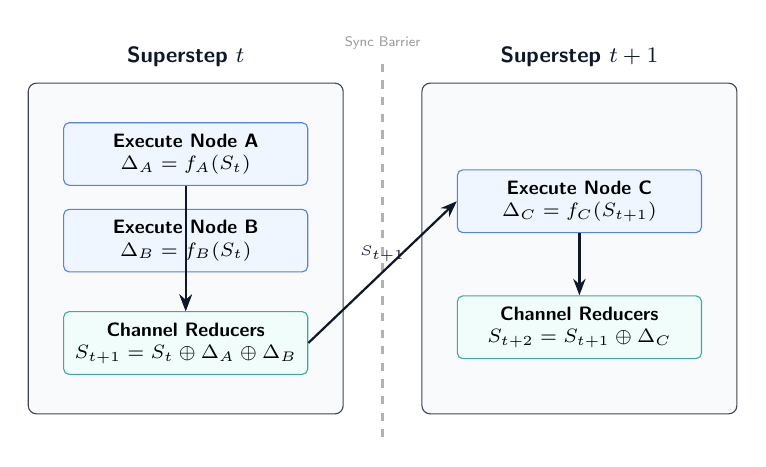
\begin{tikzpicture}[
  superstep/.style={draw=headingblue!80, fill=codebg, rounded corners=3pt, inner sep=8pt, minimum width=4.0cm, minimum height=4.2cm},
  nodeblock/.style={draw=exampleBlue!80, fill=exampleBg, rounded corners=2pt, inner sep=4pt, font=\sffamily\scriptsize\bfseries, minimum width=3.1cm, align=center},
  reducer/.style={draw=intuitionTeal!80, fill=intuitionBg, rounded corners=2pt, inner sep=4pt, font=\sffamily\scriptsize\bfseries, minimum width=3.1cm, align=center},
  arrow/.style={-{Stealth[scale=0.9]}, thick, color=headingblue}
]

\node[superstep] (s1) at (0,0) {};
\node[above=2pt of s1.north, font=\sffamily\bfseries\footnotesize, color=headingblue] {Superstep $t$};
\node[nodeblock] (n1) at (0, 1.2) {Execute Node A\\$\Delta_A = f_A(S_t)$};
\node[nodeblock] (n2) at (0, 0.1) {Execute Node B\\$\Delta_B = f_B(S_t)$};
\node[reducer] (r1) at (0, -1.2) {Channel Reducers\\$S_{t+1} = S_t \oplus \Delta_A \oplus \Delta_B$};

\draw[dashed, thick, color=gray!60] (2.5, -2.4) -- (2.5, 2.4) node[above, font=\tiny\sffamily, color=gray!80] {Sync Barrier};

\node[superstep] (s2) at (5.0,0) {};
\node[above=2pt of s2.north, font=\sffamily\bfseries\footnotesize, color=headingblue] {Superstep $t+1$};
\node[nodeblock] (n3) at (5.0, 0.6) {Execute Node C\\$\Delta_C = f_C(S_{t+1})$};
\node[reducer] (r2) at (5.0, -1.0) {Channel Reducers\\$S_{t+2} = S_{t+1} \oplus \Delta_C$};

\draw[arrow] (n1.south) -- (r1.north);
\draw[arrow] (n2.south) -- (r1.north);
\draw[arrow] (r1.east) -- (n3.west) node[above, midway, font=\tiny\sffamily] {$S_{t+1}$};
\draw[arrow] (n3.south) -- (r2.north);

\end{tikzpicture}
\caption{Pregel Superstep Model: Parallel nodes read immutable snapshot $S_t$, emit deltas, and reconcile at the synchronization barrier before $S_{t+1}$ begins.}
\label{fig:v2-ch05-pregel}
\end{figure}

\subsection{Defining State Schemas and Graph Topology}
Listing~\ref{lst:v2-ch05-schema} attaches reducers via \texttt{typing.Annotated}, and Listing~\ref{lst:v2-ch05-graph} wires our financial audit workflow.

\begin{lstlisting}[language=Python, label={lst:v2-ch05-schema}, caption={Defining Typed State Channels with Explicit Reducers}]
import operator
from typing import Annotated, Sequence, TypedDict
from langchain_core.messages import BaseMessage
from langgraph.graph.message import add_messages

def merge_dict_reducer(
    current: dict[str, str],
    update: dict[str, str] | None
) -> dict[str, str]:
    """Non-destructive dictionary merge reducer."""
    if update is None:
        return current
    merged = current.copy()
    merged.update(update)
    return merged

class FinancialAuditState(TypedDict):
    messages: Annotated[Sequence[BaseMessage], add_messages]
    discrepancies: Annotated[list[dict], operator.add]
    metadata: Annotated[dict[str, str], merge_dict_reducer]
    audit_status: str                 # Unannotated: last-writer-wins overwrite
    requires_human_approval: bool     # Unannotated: overwrite
\end{lstlisting}

\begin{commonmistakebox}[Concurrent Writes Without a Reducer]
If two nodes run in the same superstep and both return \texttt{\{"audit\_status": ...\}}, LangGraph raises \texttt{InvalidUpdateError} because an unannotated key has no merge rule for two simultaneous writes. Either attach a reducer via \texttt{Annotated} or ensure parallel nodes never write to the same scalar key.
\end{commonmistakebox}

\begin{lstlisting}[language=Python, label={lst:v2-ch05-graph}, caption={Building the Financial Audit \texttt{StateGraph} with Conditional Routing}]
from langgraph.graph import StateGraph, START, END

def intake_node(state: FinancialAuditState) -> dict:
    return {
        "metadata": {"started_at": "2026-11-23T09:00:00Z"},
        "audit_status": "in_progress"
    }

def discrepancy_detector_node(state: FinancialAuditState) -> dict:
    found = [{"id": "ERR-101", "amount": 14500.00, "vendor": "Acme Corp"}]
    needs_signoff = any(e["amount"] > 10000 for e in found)
    return {
        "discrepancies": found,
        "requires_human_approval": needs_signoff
    }

def route_after_detection(state: FinancialAuditState) -> str:
    if state.get("requires_human_approval"):
        return "human_approval_gate"
    return "auto_post_adjustments"

def human_approval_node(state: FinancialAuditState) -> dict:
    return {"audit_status": "approved_by_compliance"}

def auto_post_node(state: FinancialAuditState) -> dict:
    return {"audit_status": "posted_to_erp"}

workflow = StateGraph(FinancialAuditState)
workflow.add_node("intake", intake_node)
workflow.add_node("detector", discrepancy_detector_node)
workflow.add_node("human_approval_gate", human_approval_node)
workflow.add_node("auto_post_adjustments", auto_post_node)

workflow.add_edge(START, "intake")
workflow.add_edge("intake", "detector")
workflow.add_conditional_edges(
    "detector",
    route_after_detection,
    {
        "human_approval_gate": "human_approval_gate",
        "auto_post_adjustments": "auto_post_adjustments",
    },
)
workflow.add_edge("human_approval_gate", "auto_post_adjustments")
workflow.add_edge("auto_post_adjustments", END)
\end{lstlisting}

\subsection{Tracing \texttt{FinancialAuditState} Across Supersteps 0, 1, and 2}
Suppose we invoke the graph compiled with \texttt{interrupt\_before=["human\_approval\_gate"]} and initial input:
\texttt{discrepancies=[]}, \texttt{metadata=\{\}}, \texttt{audit\_status="pending"}, \texttt{requires\_human\_approval=False}:
\begin{enumerate}[leftmargin=18pt]
  \item \textbf{Superstep 0 (\texttt{intake} runs)}: \texttt{intake\_node} emits \texttt{metadata=\{"started\_at": "2026-11-23T09:00:00Z"\}} and \texttt{audit\_status="in\_progress"}. At the barrier, \texttt{merge\_dict\_reducer} merges into \texttt{metadata}, and \texttt{audit\_status} overwrites to \texttt{"in\_progress"}. Next node: \texttt{"detector"}.
  \item \textbf{Superstep 1 (\texttt{detector} runs)}: \texttt{discrepancy\_detector\_node} finds \texttt{ERR-101} (\$14,500) and returns \texttt{discrepancies=[...]} and \texttt{requires\_human\_approval=True}. At the barrier, \texttt{operator.add} appends \texttt{ERR-101} to \texttt{discrepancies}, \texttt{metadata} retains \texttt{"started\_at"}, and \texttt{route\_after\_detection} returns \texttt{"human\_approval\_gate"}. Because \texttt{interrupt\_before} matches \texttt{"human\_approval\_gate"}, LangGraph saves the checkpoint and pauses cleanly!
  \item \textbf{Superstep 2 (Human patch + Resume)}: The compliance officer inspects \texttt{discrepancies}, calls \texttt{aupdate\_state(..., values=\{"metadata": \{"approved\_by": "Officer Smith"\}\})}, and resumes with \texttt{astream(None, config)}. Crucially, \texttt{merge\_dict\_reducer} produces \texttt{metadata=\{"started\_at": ..., "approved\_by": "Officer Smith"\}} without erasing \texttt{"started\_at"}! \texttt{human\_approval\_gate} sets \texttt{audit\_status="approved\_by\_compliance"}, followed in the final superstep by \texttt{auto\_post\_adjustments} setting \texttt{audit\_status="posted\_to\_erp"}.
\end{enumerate}

\section{Persistence and Checkpointing with PostgreSQL}

To survive server restarts, \texttt{AsyncPostgresSaver} commits every superstep to three PostgreSQL tables (Figure~\ref{fig:v2-ch05-pg-er}):
\begin{itemize}[leftmargin=18pt]
  \item \textbf{\texttt{checkpoints}} (PK: \texttt{(thread\_id, checkpoint\_ns, checkpoint\_id)}): Stores the JSONB checkpoint metadata, channel versions, and \texttt{parent\_checkpoint\_id} pointer. (\texttt{checkpoint\_ns} isolates subgraphs cleanly within the same thread.)
  \item \textbf{\texttt{checkpoint\_blobs}} (PK: \texttt{(thread\_id, checkpoint\_ns, channel, version)}): Stores large serialized channel payloads out-of-line by \texttt{(channel, version)}. Because blobs are keyed by version rather than \texttt{checkpoint\_id}, unchanged channels are never duplicated across supersteps!
  \item \textbf{\texttt{checkpoint\_writes}} (PK: \texttt{(thread\_id, checkpoint\_ns, checkpoint\_id, task\_id, idx)}): Logs intermediate node writes emitted during a superstep for crash recovery and auditability.
\end{itemize}

\begin{figure}[htbp]
\centering
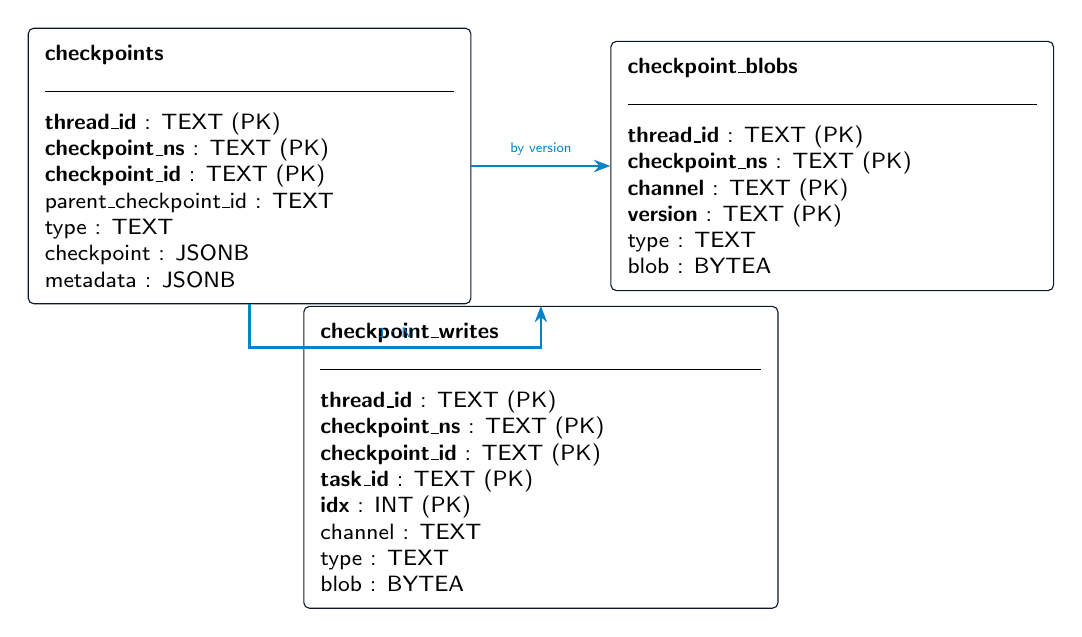
\begin{tikzpicture}[
  table/.style={draw=headingblue, fill=white, rounded corners=2pt, font=\sffamily\footnotesize, align=left, inner sep=6pt},
  arrow/.style={-{Stealth[scale=0.9]}, thick, color=linkblue}
]

\node[table] (checkpoints) at (0, 0) {
  \textbf{checkpoints}\\[2pt]
  \rule{5.2cm}{0.4pt}\\[4pt]
  \textbf{thread\_id} : TEXT (PK)\\
  \textbf{checkpoint\_ns} : TEXT (PK)\\
  \textbf{checkpoint\_id} : TEXT (PK)\\
  parent\_checkpoint\_id : TEXT\\
  type : TEXT\\
  checkpoint : JSONB\\
  metadata : JSONB
};

\node[table] (blobs) at (7.4, 0) {
  \textbf{checkpoint\_blobs}\\[2pt]
  \rule{5.2cm}{0.4pt}\\[4pt]
  \textbf{thread\_id} : TEXT (PK)\\
  \textbf{checkpoint\_ns} : TEXT (PK)\\
  \textbf{channel} : TEXT (PK)\\
  \textbf{version} : TEXT (PK)\\
  type : TEXT\\
  blob : BYTEA
};

\node[table] (writes) at (3.7, -3.7) {
  \textbf{checkpoint\_writes}\\[2pt]
  \rule{5.6cm}{0.4pt}\\[4pt]
  \textbf{thread\_id} : TEXT (PK)\\
  \textbf{checkpoint\_ns} : TEXT (PK)\\
  \textbf{checkpoint\_id} : TEXT (PK)\\
  \textbf{task\_id} : TEXT (PK)\\
  \textbf{idx} : INT (PK)\\
  channel : TEXT\\
  type : TEXT\\
  blob : BYTEA
};

\draw[arrow] (checkpoints.east) -- (blobs.west) node[above, midway, font=\tiny\sffamily] {by version};
\draw[arrow] (checkpoints.south) -- ++(0,-0.55) -| (writes.north) node[above, near start, font=\tiny\sffamily] {1 : N};

\end{tikzpicture}
\caption{Relational Schema of \texttt{PostgresSaver}: \texttt{checkpoint\_ns} scopes subgraphs, \texttt{checkpoints.checkpoint} is \texttt{JSONB}, and \texttt{checkpoint\_blobs} deduplicates payloads via PK \texttt{(thread\_id, checkpoint\_ns, channel, version)}.}
\label{fig:v2-ch05-pg-er}
\end{figure}

Listing~\ref{lst:v2-ch05-pg} wires \texttt{AsyncPostgresSaver}. Note \texttt{open=False} in \texttt{AsyncConnectionPool}: in \texttt{psycopg\_pool >= 3.2}, opening pools implicitly in \texttt{\_\_init\_\_} inside an async event loop is deprecated and triggers errors, so pass \texttt{open=False} and explicitly \texttt{await pool.open()}.

\begin{lstlisting}[language=Python, label={lst:v2-ch05-pg}, caption={Configuring \texttt{AsyncPostgresSaver} with \texttt{AsyncConnectionPool(open=False)}}]
from langgraph.checkpoint.postgres.aio import AsyncPostgresSaver
from psycopg_pool import AsyncConnectionPool

async def initialize_production_graph(connection_string: str):
    pool = AsyncConnectionPool(
        conninfo=connection_string,
        max_size=20,
        open=False,
        kwargs={"autocommit": True}
    )
    await pool.open()

    checkpointer = AsyncPostgresSaver(pool)
    await checkpointer.setup()  # Idempotent schema creation

    app = workflow.compile(
        checkpointer=checkpointer,
        interrupt_before=["human_approval_gate"]
    )
    return app, pool
\end{lstlisting}

\begin{productionwarningbox}[Checkpointer Pool Isolation]
Keep the checkpointer's \texttt{AsyncConnectionPool} separate from your application's business-query pool. If a slow ERP SQL query inside a node holds a pool connection while the superstep barrier tries to commit checkpoints, shared pools can deadlock under load.
\end{productionwarningbox}

\section{Human-in-the-Loop (HITL): \texttt{interrupt()} vs Static Breakpoints}

LangGraph offers two ways to pause for human input (Figure~\ref{fig:v2-ch05-hitl}):
\begin{enumerate}[leftmargin=18pt]
  \item \textbf{Static Breakpoints (\texttt{interrupt\_before} / \texttt{interrupt\_after})}: Compiled into the graph topology. Execution pauses cleanly at a superstep boundary before (or after) the named node. Resuming via \texttt{astream(None, config)} starts at the next scheduled node.
  \item \textbf{Dynamic Interrupts (\texttt{langgraph.types.interrupt()})}: Replaces the deprecated \texttt{NodeInterrupt} exception. A node conditionally calls \texttt{decision = interrupt(\{"amount": 14500\})} at runtime; the caller resumes using \texttt{Command(resume={"approved": True})}. \textbf{Crucial detail}: when a node using \texttt{interrupt()} resumes, LangGraph \emph{re-executes that node from its first line} so \texttt{interrupt()} can return the human's \texttt{resume} value! Therefore, never place non-idempotent side effects (like a Stripe charge) \emph{before} \texttt{interrupt()} in the same node.
\end{enumerate}

\begin{figure}[htbp]
\centering
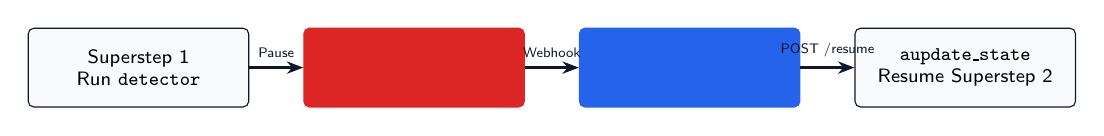
\begin{tikzpicture}[
  stepbox/.style={draw=headingblue, fill=codebg, rounded corners=2pt, minimum width=2.8cm, minimum height=1.0cm, align=center, font=\sffamily\scriptsize},
  alertbox/.style={draw=warningRed, fill=warningBg, rounded corners=2pt, minimum width=2.8cm, minimum height=1.0cm, align=center, font=\sffamily\scriptsize\bfseries, color=warningRed},
  humanbox/.style={draw=exampleBlue, fill=exampleBg, rounded corners=2pt, minimum width=2.8cm, minimum height=1.0cm, align=center, font=\sffamily\scriptsize\bfseries, color=exampleBlue},
  arrow/.style={-{Stealth[scale=0.9]}, thick, color=headingblue}
]

\node[stepbox] (start) at (0,0) {Superstep 1\\Run \texttt{detector}};
\node[alertbox] (interrupt) at (3.5,0) {Breakpoint Hit\\Checkpoint Saved};
\node[humanbox] (ui) at (7.0,0) {Human Reviewer\\Approves Delta};
\node[stepbox] (resume) at (10.5,0) {\texttt{aupdate\_state}\\Resume Superstep 2};

\draw[arrow] (start) -- (interrupt) node[above, midway, font=\tiny\sffamily] {Pause};
\draw[arrow] (interrupt) -- (ui) node[above, midway, font=\tiny\sffamily] {Webhook};
\draw[arrow] (ui) -- (resume) node[above, midway, font=\tiny\sffamily] {POST /resume};

\end{tikzpicture}
\caption{Human-in-the-Loop Interrupt Lifecycle.}
\label{fig:v2-ch05-hitl}
\end{figure}

Listing~\ref{lst:v2-ch05-hitl} demonstrates both static resumption and dynamic \texttt{langgraph.types.interrupt()}.

\begin{lstlisting}[language=Python, label={lst:v2-ch05-hitl}, caption={HITL Interrupts: Static Breakpoint Resumption and Dynamic \texttt{interrupt()}}]
from langgraph.types import Command, interrupt

def dynamic_approval_gate(state: FinancialAuditState) -> dict:
    # Side-effect-free check BEFORE interrupt(); node restarts here on resume
    high_risk = [d for d in state["discrepancies"] if d["amount"] > 10000]
    if high_risk:
        decision = interrupt({"pending_items": high_risk})
        if not decision.get("approved"):
            return {"audit_status": "rejected_by_compliance"}
    return {"audit_status": "approved_by_compliance"}

async def run_compliance_workflow(conn_str: str):
    app, pool = await initialize_production_graph(conn_str)
    config = {"configurable": {"thread_id": "session-fin-2026-991"}}
    initial_input = {
        "messages": [],
        "discrepancies": [],
        "metadata": {},
        "audit_status": "pending",
        "requires_human_approval": False,
    }

    async for event in app.astream(initial_input, config=config):
        print(f"Event: {event}")

    state_snap = await app.aget_state(config)
    print(f"Paused before: {state_snap.next}")  # ('human_approval_gate',)

    await app.aupdate_state(
        config=config,
        values={"metadata": {"approved_by": "Officer Smith"}}
    )
    async for event in app.astream(None, config=config):
        print(f"Resumed event: {event}")
    await pool.close()
\end{lstlisting}

\section{Time-Travel Debugging and History Forking}

Because \texttt{checkpoints} forms an immutable parent-linked tree (like Git commits), you can rewind any failed production thread, patch a corrupted field at an earlier \texttt{checkpoint\_id}, and replay forward from that fork without losing the original audit trail (Listing~\ref{lst:v2-ch05-timetravel}).

\begin{lstlisting}[language=Python, label={lst:v2-ch05-timetravel}, caption={Time-Travel Debugging: Inspecting History and Forking a Checkpoint}]
async def perform_time_travel(app, thread_id: str):
    config = {"configurable": {"thread_id": thread_id}}
    history = [s async for s in app.aget_state_history(config)]
    for i, snap in enumerate(history):
        print(f"Step {i}: id={snap.config['configurable']['checkpoint_id']} "
              f"next={snap.next} status={snap.values.get('audit_status')}")

    target_snap = history[-2]  # Snapshot prior to erroneous node
    fork_config = await app.aupdate_state(
        config=target_snap.config,
        values={"discrepancies": [{"id": "OVERRIDE", "amount": 0.0}]}
    )
    async for event in app.astream(None, config=fork_config):
        print(f"Forked execution: {event}")
\end{lstlisting}

\begin{realworldbox}[Recovering a Stuck CRM Agent via Checkpoint Forking]
An automated support workflow repeatedly failed when a malformed \texttt{customer\_id="cust\_"} (truncated) was saved into state early in a thread:
\begin{lstlisting}[basicstyle=\ttfamily\scriptsize]
thread_id=crm-8821 checkpoint_id=0193a4-03 next=('lookup_crm',)
ERROR: CRMClientError: 400 Bad Request for customer_id='cust_' (retry 3/3)
\end{lstlisting}
Instead of discarding the customer's 12-turn conversation, the on-call engineer queried \texttt{aget\_state\_history}, located \texttt{checkpoint\_id=0193a4-02} prior to \texttt{lookup\_crm}, patched \texttt{customer\_id="cust\_99210"} via \texttt{aupdate\_state}, and resumed from the forked config—completing the ticket cleanly.
\end{realworldbox}

\begin{tryityourselfbox}[Two-Tier Approval Routing]
Extend \texttt{FinancialAuditState} and \texttt{route\_after\_detection} so that:
\begin{enumerate}
  \item Discrepancies summing between \$1,000 and \$10,000 route to \texttt{"finance\_manager\_gate"}.
  \item Discrepancies exceeding \$10,000 route to \texttt{"cro\_gate"}.
  \item Discrepancies under \$1,000 bypass both gates straight to \texttt{"auto\_post\_adjustments"}.
\end{enumerate}
Write the Python routing function and \texttt{add\_conditional\_edges} mapping. (Worked solution in Section~5.8.)
\end{tryityourselfbox}

\section{Chapter Summary \protect\& Key Takeaways}
\begin{itemize}[leftmargin=18pt]
  \item \textbf{Reducers \& Monoids}: Reducers combine incoming deltas deterministically at superstep barriers; associative reducers prevent race conditions across parallel branches.
  \item \textbf{Pregel Supersteps}: Nodes read immutable state $S_t$, return deltas, and synchronize before $S_{t+1}$ triggers outgoing edges.
  \item \textbf{Postgres Persistence}: \texttt{AsyncPostgresSaver} stores thread snapshots in \texttt{checkpoints}, deduplicated channel versions in \texttt{checkpoint\_blobs}, and pending deltas in \texttt{checkpoint\_writes}, using \texttt{AsyncConnectionPool(open=False)}.
  \item \textbf{HITL Semantics}: Use \texttt{interrupt\_before} for node-level approval gates, or \texttt{langgraph.types.interrupt()} inside a node—keeping non-idempotent side effects \emph{after} \texttt{interrupt()} because resumption re-runs that node from the top.
  \item \textbf{Time-Travel}: Target historical \texttt{checkpoint\_id}s to fork and replay without mutating past logs.
\end{itemize}

\section{Exercises}

\subsection*{Mechanics}
\textbf{Exercise \thechapter.1}: A state schema defines \texttt{counter: int} without a reducer. Two parallel nodes $A$ and $B$ connected from \texttt{START} both return \texttt{\{"counter": 1\}}. Explain what happens at the barrier and write the exact \texttt{Annotated} reducer definition so \texttt{counter} accumulates both updates.

\textbf{Exercise \thechapter.2}: Count the PostgreSQL write operations performed by \texttt{PostgresSaver} over $S$ supersteps if $N$ nodes execute per superstep, each node writes to 2 channels, and $C$ distinct channels change value per superstep.

\subsection*{Debugging}
\textbf{Exercise \thechapter.3}: A billing graph has a single node \texttt{bill\_and\_confirm} that calls \texttt{stripe.charges.create(...)} on line 2 and then calls \texttt{interrupt("Confirm receipt?")} on line 3. When the user resumes with \texttt{Command(resume=True)}, the customer is charged twice! Explain why LangGraph re-executed the charge and show two ways to fix it.

\subsection*{Architecture}
\textbf{Exercise \thechapter.4}: Design a resilient order-fulfillment graph that validates inventory, charges a card, schedules warehouse packing, and handles an asynchronous user cancellation webhook arriving at any time before shipment.

\section{Detailed Solutions}

\subsection*{Solution \thechapter.1}
At the Superstep 0 barrier, LangGraph detects two conflicting scalar writes to \texttt{counter} and raises \texttt{InvalidUpdateError: Conflicting updates for channel 'counter'}. Fix with \texttt{operator.add}:
\begin{lstlisting}[language=Python]
import operator
from typing import Annotated, TypedDict

class CounterState(TypedDict):
    counter: Annotated[int, operator.add]
\end{lstlisting}

\subsection*{Solution \thechapter.2}
Per superstep: $2N$ rows go into \texttt{checkpoint\_writes}, $1$ row goes into \texttt{checkpoints}, and $C$ updated channel payloads go into \texttt{checkpoint\_blobs}. Over $S$ supersteps: $S \times (1 + 2N + C)$ writes. For $S=10, N=3, C=2$: $10 \times (1 + 6 + 2) = 90$ database writes.

\subsection*{Solution \thechapter.3}
Unlike static \texttt{interrupt\_after=["bill\_and\_confirm"]} (which checkpoints \emph{after} the node finishes and only re-runs if a caller mistakenly passes a fresh input dict instead of \texttt{None}), calling \texttt{langgraph.types.interrupt()} \emph{inside} a node suspends mid-function and \textbf{re-executes that node from its very first line upon resume} so \texttt{interrupt()} can yield the human's \texttt{resume} value. Thus line 2 runs twice! Two fixes: (1) split \texttt{confirm\_gate} and \texttt{charge\_card} into separate nodes and compile with \texttt{interrupt\_before=["charge\_card"]}; or (2) move \texttt{interrupt()} \emph{before} \texttt{stripe.charges.create(...)} (and pass an idempotency key derived from \texttt{thread\_id}).

\subsection*{Solution \thechapter.4}
1. \textbf{State}: \texttt{OrderState} holds \texttt{order\_id}, \texttt{is\_cancelled: bool}, \texttt{payment\_intent\_id}, and \texttt{status}. 2. \textbf{Webhook Update}: When the cancel webhook arrives, call \texttt{await app.aupdate\_state(\{"configurable": \{"thread\_id": order\_id\}\}, \{"is\_cancelled": True\})}. 3. \textbf{Conditional Guards}: Before \texttt{charge\_card} and \texttt{pack\_warehouse}, conditional edges inspect \texttt{state["is\_cancelled"]} and route to \texttt{refund\_and\_release\_inventory} $\to$ \texttt{END} if true.

\subsection*{Solution (Try It Yourself)}
\begin{lstlisting}[language=Python]
def route_after_detection(state: FinancialAuditState) -> str:
    total = sum(d["amount"] for d in state["discrepancies"])
    if total > 10000:
        return "cro_gate"
    if total >= 1000:
        return "finance_manager_gate"
    return "auto_post_adjustments"

workflow.add_conditional_edges(
    "detector",
    route_after_detection,
    {
        "cro_gate": "cro_gate",
        "finance_manager_gate": "finance_manager_gate",
        "auto_post_adjustments": "auto_post_adjustments",
    },
)
\end{lstlisting}

\begin{labbridgebox}[Hands-On Exercise \& Project Bridge]
Implement typed state channel reducers and immutable history tracking in \texttt{exercises/volume2/ex04\_agent\_state\_reducer.py}, then explore a full stateful graph with HITL approval gates and time-travel in \texttt{projects/p05-langgraph-agent-state/} (\texttt{agent/state.py}, \texttt{agent/graph.py}, \texttt{agent/tools.py}, \texttt{tests/test\_agent\_graph.py}).
\end{labbridgebox}

\section{Further Reading \protect\& Citations}
\begin{itemize}[leftmargin=18pt]
  \item Malewicz, G., et al. (2010). \emph{Pregel: A System for Large-Scale Graph Processing}. ACM SIGMOD.
  \item Valiant, L. G. (1990). \emph{A Bridging Model for Parallel Computation}. Communications of the ACM, 33(8), 103--111.
  \item LangChain AI. (2025). \emph{LangGraph Persistence and Human-in-the-Loop Documentation}. \url{https://langchain-ai.github.io/langgraph/}.
\end{itemize}

\chapter{LLM Evaluations: The RAG Triad, Metrics, and Evals-Driven Development}
\label{ch:llm_evaluations}

\begin{chaptergoalsbox}
\textbf{What You Will Learn:}
\begin{itemize}[leftmargin=15pt]
  \item Why deterministic unit testing, BLEU, and ROUGE fail on modern generative language systems.
  \item The RAG Triad (TruLens) and component evaluation metrics (Ragas): Faithfulness, Answer Relevance, Context Precision, and Context Recall.
  \item Mathematical formalization of claim extraction and natural language entailment verification.
  \item Synthetic test dataset synthesis using Evol-Instruct multi-hop generation.
  \item Mitigating LLM-as-a-Judge systematic vulnerabilities: Position bias, verbosity bias, and self-enhancement bias.
  \item Implementing automated CI/CD evaluation gates and statistical regression boundaries.
\end{itemize}

\textbf{What You Should Already Understand:}
\begin{itemize}[leftmargin=15pt]
  \item Precision, Recall, and $F_1$ classification metrics.
  \item Basic prompt engineering and structured JSON output generation.
  \item CI/CD pipeline automation (GitHub Actions, GitLab CI).
\end{itemize}

\textbf{Why This Topic Exists:}
In traditional software, \texttt{assert add(2, 2) == 4} provides binary truth. In LLM applications, changing a single word in a system prompt or upgrading from GPT-4o to Claude 3.5 Sonnet may improve 80\% of customer responses while subtly introducing catastrophic hallucinations into 5\% of edge cases. Without automated semantic evaluation metrics, engineering teams fly blind.

\textbf{Motivating Practical Problem:}
A health-insurance chatbot answers queries regarding policy coverage. An engineer updates the prompt to make responses "more empathetic and concise." While internal spot-checks look excellent, the new prompt silently causes the model to tell customers that experimental chemotherapy treatments are covered without prior authorization. By the time customer complaints escalate, the company faces significant regulatory fines.
\end{chaptergoalsbox}

\section{The Generative Evaluation Crisis}

Traditional software engineering relies on deterministic assertion testing: given input $X$, output must strictly equal $Y$. In generative AI, this paradigm collapses:
\begin{itemize}[leftmargin=18pt]
  \item \textbf{Non-Deterministic Semantic Equivalence}: The sentences \emph{"The engine requires 5W-30 synthetic oil"} and \emph{"Use 5W-30 full synthetic lubricant for the powertrain"} share identical semantic truth, but zero exact string equality.
  \item \textbf{Failure of $n$-gram Overlap Metrics (BLEU and ROUGE)}: BLEU and ROUGE measure superficial surface-level $n$-gram overlap. If a model generates:
  \begin{center}
  \emph{"Patient should take 50mg of Atenolol"} $\longleftrightarrow$ \emph{"Patient should not take 50mg of Atenolol"}
  \end{center}
  The ROUGE-1 score is 0.86 (near perfect), despite the medical advice being completely inverted and potentially lethal.
\end{itemize}

To evaluate generative pipelines at scale, the industry transitioned to \textbf{Evals-Driven Development (EDD)}, employing smaller, highly-calibrated LLMs to audit generation traces against formal semantic contracts.

\section{The RAG Triad and Core Metrics}

Formalized by TruLens and expanded by frameworks like Ragas (Es et al., 2023), the \textbf{RAG Triad} models the three interdependent pillars of a retrieval-augmented system:

\begin{figure}[htbp]
\centering
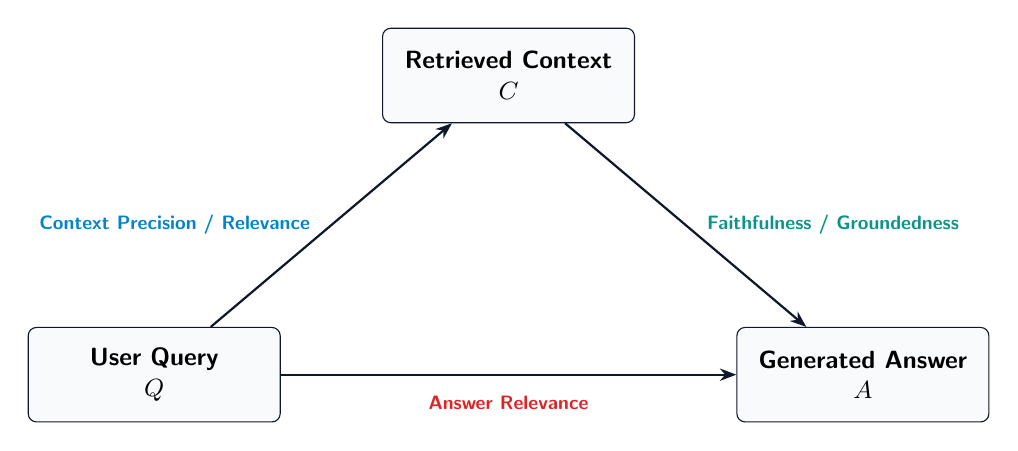
\begin{tikzpicture}[
  entity/.style={draw=headingblue, fill=codebg, rounded corners=3pt, font=\sffamily\small\bfseries, minimum width=3.2cm, minimum height=1.2cm, align=center},
  metric/.style={draw=warningRed, fill=warningBg, rounded corners=2pt, font=\sffamily\scriptsize\bfseries, minimum width=3.0cm, minimum height=0.8cm, align=center, color=warningRed},
  arrow/.style={-{Stealth[scale=0.9]}, thick, color=headingblue}
]

\node[entity] (query) at (0, 0) {User Query\\$Q$};
\node[entity] (context) at (4.5, 3.8) {Retrieved Context\\$C$};
\node[entity] (answer) at (9.0, 0) {Generated Answer\\$A$};

% Metrics along edges
\draw[arrow] (query) -- (context) node[midway, left=4pt, font=\sffamily\scriptsize\bfseries, color=linkblue] {Context Precision / Relevance};
\draw[arrow] (context) -- (answer) node[midway, right=4pt, font=\sffamily\scriptsize\bfseries, color=intuitionTeal] {Faithfulness / Groundedness};
\draw[arrow] (query) -- (answer) node[midway, below=4pt, font=\sffamily\scriptsize\bfseries, color=warningRed] {Answer Relevance};

\end{tikzpicture}
\caption{The RAG Triad: Context Relevance, Faithfulness, and Answer Relevance form a closed evaluation loop.}
\label{fig:rag_triad}
\end{figure}

\subsection{1. Faithfulness (Groundedness)}
Faithfulness measures whether the generated answer $A$ is strictly derived from the retrieved context $C$, preventing hallucinations.

\begin{figure}[htbp]
\centering
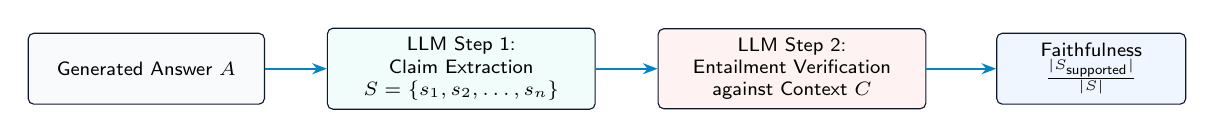
\begin{tikzpicture}[
  box/.style={draw=headingblue, fill=codebg, rounded corners=2pt, font=\sffamily\scriptsize, align=center, minimum height=0.9cm},
  arrow/.style={-{Stealth[scale=0.8]}, thick, color=linkblue}
]

\node[box, minimum width=3.0cm] (ans) at (0, 0) {Generated Answer $A$};
\node[box, minimum width=3.4cm, fill=intuitionBg] (claims) at (4.0, 0) {LLM Step 1:\\Claim Extraction\\$S = \{s_1, s_2, \dots, s_n\}$};
\node[box, minimum width=3.4cm, fill=warningBg] (entail) at (8.2, 0) {LLM Step 2:\\Entailment Verification\\against Context $C$};
\node[box, minimum width=2.4cm, fill=exampleBg] (score) at (12.0, 0) {Faithfulness\\$\frac{|S_{\text{supported}}|}{|S|}$};

\draw[arrow] (ans) -- (claims);
\draw[arrow] (claims) -- (entail);
\draw[arrow] (entail) -- (score);

\end{tikzpicture}
\caption{Two-Step Algorithmic Verification of Faithfulness.}
\label{fig:faithfulness_pipeline}
\end{figure}

The calculation proceeds in two deterministic steps:
\begin{enumerate}[leftmargin=18pt]
  \item \textbf{Decomposition}: The evaluation LLM decomposes $A$ into atomic factual propositions $S = \{s_1, s_2, \dots, s_{|S|}\}$.
  \item \textbf{Entailment Check}: For each claim $s_i$, the evaluation model determines whether $C \models s_i$ (Natural Language Inference entailment).
\end{enumerate}
\begin{equation}
\text{Faithfulness}(A, C) = \frac{|\{s_i \in S \mid C \models s_i\}|}{|S|} \in [0, 1]
\end{equation}

\subsection{2. Answer Relevance}
Answer relevance measures whether the response directly addresses the user's inquiry, irrespective of factual truth. A response stating \emph{"Paris is the capital of France and the Eiffel Tower is 330m tall"} is 100\% faithful, but if the user asked \emph{"How do I reset my router password?"}, its Answer Relevance is 0.0.

To compute this without human labels, Ragas generates $M$ hypothetical reverse questions $q_1, \dots, q_M$ from the generated answer $A$ and measures mean cosine similarity against the original query $Q$:
\begin{equation}
\text{Answer\_Relevance}(A, Q) = \frac{1}{M} \sum_{i=1}^M \frac{\vec{E}(q_i) \cdot \vec{E}(Q)}{\|\vec{E}(q_i)\| \|\vec{E}(Q)\|}
\end{equation}

\subsection{3. Context Precision (Context Relevance)}
Context Precision evaluates the retrieval stage. Given retrieved chunks $C = [c_1, c_2, \dots, c_K]$, it calculates the Mean Average Precision (MAP) of whether relevant chunks are ranked at the top:
\begin{equation}
\text{Context\_Precision@K} = \frac{\sum_{k=1}^K (\text{Precision@}k \times v_k)}{\sum_{k=1}^K v_k}
\end{equation}
where $v_k \in \{0, 1\}$ denotes whether chunk $c_k$ contains ground-truth information necessary to answer the question.

\begin{lstlisting}[language=Python, caption={Faithfulness Evaluator Implementation from Scratch}]
import json
from pydantic import BaseModel
from typing import list

class ClaimList(BaseModel):
    claims: list[str]

class ClaimVerification(BaseModel):
    claim: str
    is_supported: bool
    verbatim_quote: str
    reasoning: str

class VerificationResult(BaseModel):
    verifications: list[ClaimVerification]

EXTRACT_CLAIMS_PROMPT = """
You are a strict factual auditor. Break down the following text into atomic, independent factual claims.
Each claim must contain exactly one verifiable fact.
Text: {answer}
Respond strictly in JSON matching the schema.
"""

VERIFY_CLAIMS_PROMPT = """
You are a formal logic judge. For each of the following claims, determine whether it is strictly supported by the provided context.
Context:
{context}

Claims to verify:
{claims_json}

A claim is supported ONLY if it can be directly inferred from the context. If the context does not mention the fact, is_supported must be FALSE.
"""

async def evaluate_faithfulness(llm_judge, context: str, answer: str) -> float:
    # Step 1: Extract atomic propositions
    prompt_1 = EXTRACT_CLAIMS_PROMPT.format(answer=answer)
    res_1 = await llm_judge.generate_structured(prompt_1, schema=ClaimList)
    claims = res_1.claims
    
    if not claims:
        return 1.0 # Vacuously true
        
    # Step 2: Verify each claim against context
    prompt_2 = VERIFY_CLAIMS_PROMPT.format(
        context=context, 
        claims_json=json.dumps(claims)
    )
    res_2 = await llm_judge.generate_structured(prompt_2, schema=VerificationResult)
    
    supported_count = sum(1 for v in res_2.verifications if v.is_supported)
    return supported_count / len(claims)
\end{lstlisting}

\section{Synthetic Test Dataset Generation}

Evaluating systems requires high-quality ground-truth evaluation sets (Query, Ground-Truth Context, Ground-Truth Answer). Relying entirely on manual human labeling costs tens of thousands of dollars and moves too slowly for rapid iteration.

\textbf{Evol-Instruct Synthesis} (Xu et al., 2023) generates realistic, multi-faceted benchmark datasets directly from ingested technical documents:

\begin{figure}[htbp]
\centering
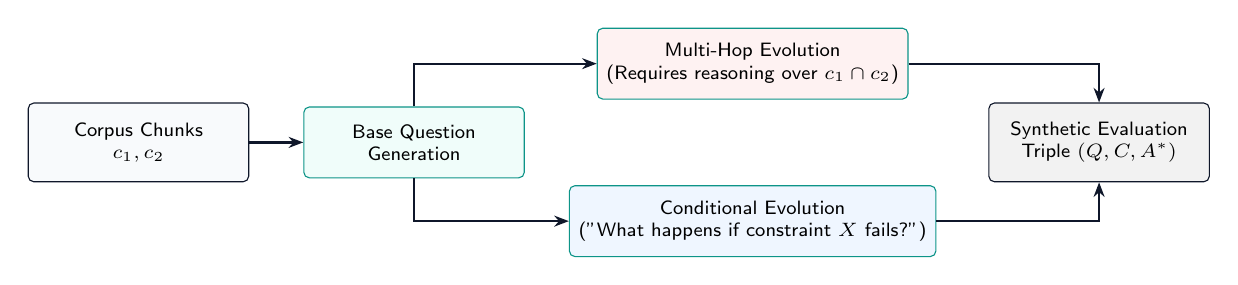
\begin{tikzpicture}[
  chunk/.style={draw=headingblue, fill=codebg, rounded corners=2pt, font=\sffamily\scriptsize, minimum width=2.8cm, minimum height=1.0cm, align=center},
  evol/.style={draw=intuitionTeal, fill=intuitionBg, rounded corners=2pt, font=\sffamily\scriptsize, minimum width=2.8cm, minimum height=0.9cm, align=center},
  arrow/.style={-{Stealth[scale=0.8]}, thick, color=headingblue}
]

\node[chunk] (doc) at (0, 1.5) {Corpus Chunks\\$c_1, c_2$};
\node[evol] (base) at (3.5, 1.5) {Base Question\\Generation};
\node[evol, fill=warningBg, minimum width=3.8cm] (multi) at (7.8, 2.5) {Multi-Hop Evolution\\(Requires reasoning over $c_1 \cap c_2$)};
\node[evol, fill=exampleBg, minimum width=3.8cm] (cond) at (7.8, 0.5) {Conditional Evolution\\("What happens if constraint $X$ fails?")};
\node[chunk, fill=gray!10] (final) at (12.2, 1.5) {Synthetic Evaluation\\Triple $(Q, C, A^*)$};

\draw[arrow] (doc) -- (base);
\draw[arrow] (base) |- (multi);
\draw[arrow] (base) |- (cond);
\draw[arrow] (multi) -| (final);
\draw[arrow] (cond) -| (final);

\end{tikzpicture}
\caption{Evol-Instruct Synthetic Question Generation Pipeline.}
\label{fig:evol_instruct}
\end{figure}

\begin{lstlisting}[language=Python, caption={Generating Multi-Hop Synthetic Evaluation Triples}]
SYNTHETIC_EVOLVE_PROMPT = """
You are an expert curriculum examiner. Given these two related document fragments, generate a complex MULTI-HOP question.
The question MUST NOT be answerable by reading Chunk 1 alone, nor by reading Chunk 2 alone.
Answering the question MUST require combining a fact from Chunk 1 with a fact from Chunk 2.

Chunk 1:
{chunk_1}

Chunk 2:
{chunk_2}

Provide your output as:
Question: <complex multi-hop question>
GroundTruthAnswer: <comprehensive answer citing both chunks>
"""

async def generate_synthetic_triple(llm, chunk_1: str, chunk_2: str) -> dict:
    prompt = SYNTHETIC_EVOLVE_PROMPT.format(chunk_1=chunk_1, chunk_2=chunk_2)
    response = await llm.generate(prompt)
    # Parse into (question, ground_truth, [chunk_1, chunk_2])
    return parse_synthetic_response(response, [chunk_1, chunk_2])
\end{lstlisting}

\section{LLM-as-a-Judge Calibration \& Bias Mitigation}

While using an LLM to evaluate another LLM is scalable, naive judges exhibit severe systematic cognitive biases (Zheng et al., 2023):

\begin{enumerate}[leftmargin=18pt]
  \item \textbf{Position Bias (Order Effect)}: When comparing Candidate A vs Candidate B pairwise, models preferentially favor Candidate A up to 65\% of the time simply because it appears first in the prompt.
  \item \textbf{Verbosity Bias}: Models systematically award higher scores to longer, fluffier responses containing conversational pleasantries over crisp, accurate 1-line answers.
  \item \textbf{Self-Enhancement Bias}: Models preferentially award higher scores to completions generated by their own model family (e.g., GPT-4 favoring GPT-3.5 over Claude 3.5).
\end{enumerate}

\subsection{Engineering Mitigation Protocols}
\begin{itemize}[leftmargin=18pt]
  \item \textbf{Pairwise Position Swap}: Evaluate twice: trial 1 with $(A, B)$, trial 2 with $(B, A)$. A win is counted if and only if Candidate $A$ wins both positions. If candidates split decisions, mark as a tie.
  \item \textbf{G-Eval / Chain-of-Thought Rubrics}: Force the judge to output a structured step-by-step reasoning trace evaluating explicit criteria before emitting numeric scores.
  \item \textbf{Few-Shot Calibration Anchors}: Provide the judge with fixed, standardized reference examples representing a score of 1, 3, and 5 to pin scale variance.
\end{itemize}

\begin{figure}[htbp]
\centering
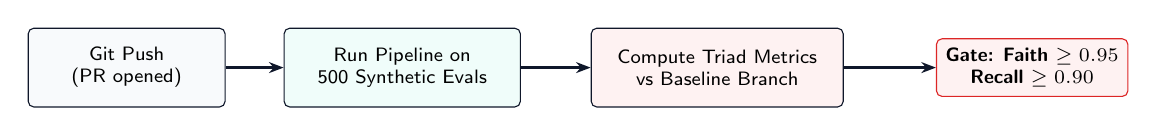
\begin{tikzpicture}[
  stage/.style={draw=headingblue, fill=codebg, rounded corners=2pt, font=\sffamily\scriptsize, minimum height=1.0cm, align=center},
  arrow/.style={-{Stealth[scale=0.8]}, thick, color=headingblue}
]

\node[stage, minimum width=2.5cm] (git) at (0, 0) {Git Push\\(PR opened)};
\node[stage, minimum width=3.0cm, fill=intuitionBg] (runner) at (3.5, 0) {Run Pipeline on\\500 Synthetic Evals};
\node[stage, minimum width=3.2cm, fill=warningBg] (calc) at (7.5, 0) {Compute Triad Metrics\\vs Baseline Branch};
\node[draw=warningRed, fill=warningBg, rounded corners=2pt, font=\sffamily\scriptsize\bfseries, minimum width=2.4cm, align=center] (gate) at (11.5, 0) {Gate: Faith $\ge 0.95$\\Recall $\ge 0.90$};

\draw[arrow] (git) -- (runner);
\draw[arrow] (runner) -- (calc);
\draw[arrow] (calc) -- (gate);

\end{tikzpicture}
\caption{Continuous Integration (CI/CD) Automated Evaluation Gate.}
\label{fig:cicd_evals}
\end{figure}

\begin{productionwarningbox}[Never Use Zero-Shot Likert Scales]
Prompts instructing an LLM to \emph{"Rate the quality of this response from 1 to 10"} are useless in production. LLM scores on unanchored 1-10 scales cluster entirely between 7 and 9 with immense stochastic variance. Always use binary assertions (Supported vs Not Supported) or strict qualitative rubrics with explicit failure definitions.
\end{productionwarningbox}

\begin{realworldbox}[Catching a Silent Regression in Production]
A major retail banking application deployed a prompt optimization to reduce token usage by 18\%.
The standard regression test suite (1,000 synthetic questions run through GitHub Actions) ran automatically. While overall Answer Relevance held steady at 0.94, the Context Recall metric for credit card dispute policies dropped from 0.98 to 0.76.
The CI evaluation gate failed the pull request build, blocking a regression that would have cost the bank thousands of dollars in uncollected dispute fees.
\end{realworldbox}

\begin{tryityourselfbox}[Build an Automated PR Evaluation Gate]
Write a GitHub Actions workflow script using Python:
\begin{enumerate}
  \item Load a golden dataset of 25 QA pairs from \texttt{evals/golden\_dataset.json}.
  \item Execute the application's RAG pipeline against each query.
  \item Score Faithfulness and Context Precision using the \texttt{evaluate\_faithfulness} function.
  \item If the mean Faithfulness drops below 0.92, raise \texttt{sys.exit(1)} to block PR merge.
\end{enumerate}
\end{tryityourselfbox}

\section{Chapter Summary \& Key Takeaways}
\begin{itemize}[leftmargin=18pt]
  \item \textbf{Failure of Deterministic Tests}: String matching, BLEU, and ROUGE fail to capture semantic truth and penalize valid paraphrasing. Evals-Driven Development (EDD) uses LLM judges operating on formal semantic contracts.
  \item \textbf{The RAG Triad}: Faithfulness audits the Answer against Context. Context Precision audits retrieval against the Query. Answer Relevance audits the Answer against the Query.
  \item \textbf{Atomic Claim Verification}: Faithfulness is evaluated by breaking answers into atomic propositions and executing natural language entailment against retrieved context chunks.
  \item \textbf{Synthetic Benchmarking}: Evol-Instruct synthesizes multi-hop, reasoning-heavy test datasets from raw documents, enabling automated testing without expensive manual labeling.
  \item \textbf{Judge Calibration}: Mitigate LLM judge vulnerabilities (position bias, verbosity bias) via pairwise swaps, chain-of-thought grading rubrics, and strict anchor definitions.
  \item \textbf{CI/CD Gates}: Treat semantic evaluation scores like unit test coverage; block deployment pipelines whenever Faithfulness or Context Precision drops below calibrated thresholds.
\end{itemize}

\section{Exercises}

\subsection*{Mechanics}
\textbf{Exercise 6.1}: A generated answer contains 5 atomic claims:
\begin{itemize}
  \item $s_1$: "PostgreSQL uses Write-Ahead Logging for durability."
  \item $s_2$: "The default WAL buffer size is 16 Megabytes."
  \item $s_3$: "PostgreSQL stores tables in 16 Kilobyte page blocks."
  \item $s_4$: "Checkpointing flushes dirty pages from shared buffers to disk."
  \item $s_5$: "MVCC creates a new tuple version for every SQL UPDATE."
\end{itemize}
Upon entailment check against the retrieved context, claims $s_1, s_2, s_4,$ and $s_5$ are supported, while the context explicitly states that page blocks are 8 Kilobytes ($s_3$ fails). Calculate the Faithfulness score.

\textbf{Exercise 6.2}: Given a retrieval system that returns 4 chunks for a query, where chunks at rank 1, 2, and 4 are relevant ($v_1=1, v_2=1, v_3=0, v_4=1$), compute the Context Precision@4 score.

\subsection*{Debugging}
\textbf{Exercise 6.3}: In an A/B evaluation between Model Alpha and Model Beta, Model Alpha wins 82\% of pairwise comparisons. However, an engineer notices that Model Alpha was consistently placed as "Option 1" in the judge prompt. When the order is reversed, Model Beta wins 79\% of comparisons. Explain this discrepancy and prescribe the exact evaluation protocol to eliminate it.

\subsection*{Architecture}
\textbf{Exercise 6.4}: Design a continuous offline evaluation engine for a high-volume enterprise customer service agent processing 200,000 conversations daily. Your architecture must sample traces, execute Faithfulness/Relevance checks, detect drift, and alert engineers without saturating LLM API rate limits or budget caps.

\section{Detailed Solutions}

\subsection*{Solution 6.1}
The total number of extracted atomic claims $|S| = 5$.
The number of supported claims $|S_{\text{supported}}| = 4$ ($s_1, s_2, s_4, s_5$).
\[
\text{Faithfulness} = \frac{|S_{\text{supported}}|}{|S|} = \frac{4}{5} = 0.80 \quad (80\%)
\]

\subsection*{Solution 6.2}
Precision@$k$ is the fraction of relevant documents in the top-$k$ results:
\begin{itemize}
  \item $k=1: v_1=1 \implies \text{Precision@}1 = \frac{1}{1} = 1.0$
  \item $k=2: v_2=1 \implies \text{Precision@}2 = \frac{2}{2} = 1.0$
  \item $k=3: v_3=0 \implies \text{Precision@}3 = \frac{2}{3} \approx 0.667$ (not included in sum since $v_3=0$)
  \item $k=4: v_4=1 \implies \text{Precision@}4 = \frac{3}{4} = 0.75$
\end{itemize}
Context Precision@4 is:
\[
\text{Context Precision@4} = \frac{\sum_{k=1}^4 (\text{Precision@}k \times v_k)}{\sum_{k=1}^4 v_k} = \frac{1.0(1) + 1.0(1) + 0.667(0) + 0.75(1)}{1 + 1 + 0 + 1} = \frac{2.75}{3} \approx 0.9167
\]

\subsection*{Solution 6.3}
The system is suffering from \textbf{Position Bias}: LLM judges preferentially select the first option presented in the context window.
Fix: Implement the \textbf{Pairwise Swap Protocol}:
\begin{enumerate}
  \item Run Test 1: Present Option 1 = Alpha, Option 2 = Beta.
  \item Run Test 2: Present Option 1 = Beta, Option 2 = Alpha.
  \item Evaluation logic:
  \[
  \text{Score} = \begin{cases} 
  \text{Alpha Win} & \text{if Alpha wins Test 1 AND Alpha wins Test 2} \\
  \text{Beta Win} & \text{if Beta wins Test 1 AND Beta wins Test 2} \\
  \text{Tie / Inconclusive} & \text{if winners disagree across positions}
  \end{cases}
  \]
\end{enumerate}

\subsection*{Solution 6.4}
Architecture:
\begin{enumerate}
  \item \textbf{Stratified Sampling Queue}: Out of 200,000 daily traces, capture 1\% (2,000 traces) using reservoir sampling stratified across user intent categories and explicit negative feedback flags.
  \item \textbf{Decoupled Worker Pool}: Push sampled trace IDs to an Amazon SQS / Celery queue processed by background workers running a lightweight, high-throughput judge (e.g., Llama-3.1-70B or GPT-4o-mini).
  \item \textbf{Statistical Process Control (SPC)}: Aggregate daily scores into rolling 7-day Shewhart control charts. If the mean Faithfulness drops by more than $3\sigma$ below the moving average, trigger a PagerDuty alert to the AI platform team.
\end{enumerate}

\section{Further Reading \& Citations}
\begin{itemize}[leftmargin=18pt]
  \item Es, S., et al. (2023). \emph{Ragas: Automated Evaluation of Retrieval Augmented Generation}. arXiv preprint arXiv:2309.15217.
  \item Zheng, L., et al. (2023). \emph{Judging LLM-as-a-Judge with MT-Bench and Chatbot Arena}. Advances in Neural Information Processing Systems (NeurIPS).
  \item Xu, C., et al. (2023). \emph{WizardLM: Empowering Large Language Models to Follow Complex Instructions (Evol-Instruct)}. arXiv preprint arXiv:2304.12244.
\end{itemize}

\chapter{Observability and Tracing: OpenTelemetry, Latency, and LLMOps}
\label{chap:observability}

\begin{chaptergoalsbox}
\textbf{What You Will Learn:}
\begin{itemize}[leftmargin=15pt]
  \item Why traditional HTTP 200 monitoring breaks on probabilistic, streaming AI APIs.
  \item OpenTelemetry from first principles: Traces, Spans, \texttt{TraceID}/\texttt{SpanID}, W3C \texttt{traceparent} headers, and \texttt{asyncio} \texttt{contextvars}.
  \item OpenTelemetry Generative AI Semantic Conventions (\texttt{gen\_ai.usage.input\_tokens}, \texttt{gen\_ai.usage.output\_tokens}) and FastAPI instrumentation.
  \item Streaming latency profiling: GPU prefill vs decode, KV-cache prefix reuse, Time to First Token (TTFT), and Inter-Token Latency (ITL).
  \item Token economics, prompt caching pricing ledgers, PII redaction, and tail-based sampling.
\end{itemize}

\textbf{What You Should Already Understand:}
\begin{itemize}[leftmargin=15pt]
  \item Basic Python functions, classes, and HTTP client/server requests.
  \item Chapters~3--6 (RAG pipelines, tool-calling agents, and evaluation metrics).
\end{itemize}

\textbf{Why This Topic Exists:}
In conventional web APIs, an HTTP \texttt{200 OK} response in under a second means the system is healthy. In AI engineering, an HTTP \texttt{200 OK} can mask a 40-second tail latency spike, a \$15 runaway agent loop, a silent vector-index fallback, or a leaked credit card number inside a prompt. Distributed tracing gives engineers X-ray vision across every retrieval call, tool invocation, and token stream.

\textbf{Motivating Practical Problem:}
A legal research assistant's $p99$ response latency (the threshold covering the fastest 99\% of requests while the slowest 1\% exceed it) jumps from 3.2 seconds to 28.5 seconds on a Tuesday afternoon. Without a per-request span waterfall separating vector search, LLM prefill, LLM decode, and SQL tool execution, engineers cannot tell which dependency stalled.
\end{chaptergoalsbox}

\section{Why Black-Box APM Fails on AI Systems}

Traditional Application Performance Monitoring (APM) treats an LLM invocation as one opaque outbound call: \texttt{POST https://api.openai.com/v1/chat/completions -> 200 OK}. That hides three realities:
\begin{itemize}[leftmargin=18pt]
  \item \textbf{HTTP 200 Can Still Be Broken}: A 200 response can contain a safety refusal, invalid JSON, or an empty completion.
  \item \textbf{Wildly Asymmetric Costs}: Two 1.5-second requests can differ in cost by $500\times$ if one hits a 200-token cached prompt (\$0.0003) while the other sends 64,000 uncached tokens (\$0.16).
  \item \textbf{Streaming Perception}: Most AI UIs stream words via \textbf{Server-Sent Events (SSE)}—a standard HTTP response kept open so the server pushes \texttt{data:} chunks as each token is produced. Total request duration misses how long the user stared at a blank screen waiting for the very first word.
\end{itemize}

\section{OpenTelemetry From First Principles}

Before recording AI attributes, understand the four building blocks of \textbf{OpenTelemetry (OTel)}, the industry-standard open telemetry specification:

\begin{enumerate}[leftmargin=18pt]
  \item \textbf{Trace and \texttt{TraceID}}: A \textbf{Trace} represents the complete end-to-end journey of one user request across services, identified globally by a 128-bit hexadecimal \texttt{TraceID} (e.g., \texttt{4bf92f3577b34da6a3ce929d0e0e4736}).
  \item \textbf{Span and \texttt{SpanID}}: A \textbf{Span} represents one named, timed operation inside that trace (such as \texttt{VectorSearch}, \texttt{chat.completion}, or \texttt{ToolExecution}). Each span carries its own 64-bit \texttt{SpanID}, its \texttt{ParentSpanID}, start/end timestamps, structured key-value \textbf{attributes}, and timestamped \textbf{events} (like \texttt{"first\_token"}). Plotting parent and child spans by start time produces a \textbf{waterfall diagram} (Figure~\ref{fig:v2-ch07-spans}).
  \item \textbf{W3C \texttt{traceparent} Header}: When Service A calls Service B over HTTP, how does Service B know which trace and parent span it belongs to? Service A injects the W3C TraceContext HTTP header:
  \begin{center}\small\ttfamily
  traceparent: 00-4bf92f3577b34da6a3ce929d0e0e4736-00f067aa0ba902b7-01
  \end{center}
  Its four hyphenated fields are: \texttt{version} (\texttt{00}), \texttt{trace-id} (32 hex chars), \texttt{parent-span-id} (16 hex chars), and \texttt{trace-flags} (\texttt{01} = sampled).
  \item \textbf{Async Context Propagation (\texttt{contextvars})}: Inside a Python \texttt{asyncio} server, hundreds of user requests interleave concurrently on a single thread. A global variable \texttt{CURRENT\_SPAN} would scramble traces across users! Instead, Python provides \texttt{contextvars.ContextVar}—a task-local slot that Python's event loop automatically swaps whenever it switches between coroutines. OpenTelemetry stores the active span inside a \texttt{ContextVar}. \textbf{Watch out}: if you offload work to a separate OS thread (\texttt{loop.run\_in\_executor}) or a background worker queue, a new thread starts with an \emph{empty} \texttt{ContextVar}, breaking the parent-child link unless you explicitly capture \texttt{ctx = otel\_context.get\_current()} and re-attach it inside the worker.
\end{enumerate}

\begin{figure}[htbp]
\centering
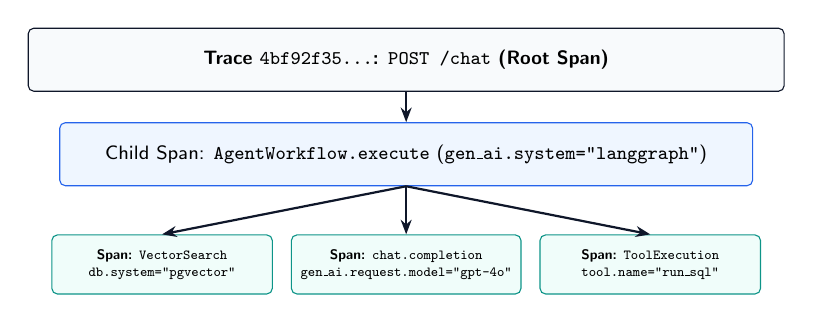
\begin{tikzpicture}[
  root/.style={draw=headingblue, fill=codebg, rounded corners=2pt, font=\sffamily\scriptsize\bfseries, minimum width=9.6cm, minimum height=0.8cm},
  agent/.style={draw=exampleBlue, fill=exampleBg, rounded corners=2pt, font=\sffamily\scriptsize, minimum width=8.8cm, minimum height=0.8cm},
  child/.style={draw=intuitionTeal, fill=intuitionBg, rounded corners=2pt, font=\sffamily\tiny\bfseries, minimum width=2.8cm, minimum height=0.75cm, align=center},
  arrow/.style={-{Stealth[scale=0.8]}, thick, color=headingblue}
]

\node[root] (session) at (0, 3.2) {Trace \texttt{4bf92f35...}: \texttt{POST /chat} (Root Span)};
\node[agent] (chain) at (0, 2.0) {Child Span: \texttt{AgentWorkflow.execute} (\texttt{gen\_ai.system="langgraph"})};

\node[child] (s1) at (-3.1, 0.6) {Span: \texttt{VectorSearch}\\\texttt{db.system="pgvector"}};
\node[child] (s2) at (0, 0.6) {Span: \texttt{chat.completion}\\\texttt{gen\_ai.request.model="gpt-4o"}};
\node[child] (s3) at (3.1, 0.6) {Span: \texttt{ToolExecution}\\\texttt{tool.name="run\_sql"}};

\draw[arrow] (session.south) -- (chain.north);
\draw[arrow] (chain.south) -- (s1.north);
\draw[arrow] (chain.south) -- (s2.north);
\draw[arrow] (chain.south) -- (s3.north);

\end{tikzpicture}
\caption{OpenTelemetry Span Hierarchy for an AI Agent Request.}
\label{fig:v2-ch07-spans}
\end{figure}

\subsection{OpenTelemetry Semantic Conventions for Generative AI}
Standardizing attribute names via OTel GenAI Semantic Conventions lets you switch backends (Langfuse, Grafana Tempo, Datadog, Honeycomb) without rewriting application instrumentation (Table~\ref{tab:v2-ch07-otel}).

\begin{table}[htbp]
\centering
\small
\begin{tabular}{lll}
\toprule
\textbf{Attribute Name} & \textbf{Type} & \textbf{Description / Example} \\
\midrule
\texttt{gen\_ai.system} & string & Provider identifier (\texttt{openai}, \texttt{anthropic}, \texttt{cohere}) \\
\texttt{gen\_ai.operation.name} & string & Operation (\texttt{chat}, \texttt{embeddings}, \texttt{execute\_tool}) \\
\texttt{gen\_ai.request.model} & string & Model name (\texttt{gpt-4o}, \texttt{claude-3-5-sonnet-20241022}) \\
\texttt{gen\_ai.request.temperature} & float & Sampling temperature ($0.0 \le T \le 2.0$) \\
\texttt{gen\_ai.request.max\_tokens} & int & Maximum output token limit \\
\texttt{gen\_ai.response.id} & string & Provider completion ID (\texttt{chatcmpl-9A8X...}) \\
\texttt{gen\_ai.usage.input\_tokens} & int & Input prompt tokens consumed \\
\texttt{gen\_ai.usage.output\_tokens} & int & Output completion tokens generated \\
\bottomrule
\end{tabular}
\caption{OpenTelemetry Generative AI Semantic Attributes.}
\label{tab:v2-ch07-otel}
\end{table}

Listing~\ref{lst:v2-ch07-fastapi} shows real \texttt{opentelemetry-sdk} instrumentation inside a FastAPI endpoint, including child spans, span events for TTFT, and explicit context propagation across a worker thread.

\begin{lstlisting}[language=Python, label={lst:v2-ch07-fastapi}, caption={FastAPI OpenTelemetry Instrumentation with Context Propagation}]
import asyncio
import time
from fastapi import FastAPI
from opentelemetry import context as otel_context, trace
from opentelemetry.sdk.trace import TracerProvider
from opentelemetry.sdk.trace.export import BatchSpanProcessor, ConsoleSpanExporter

provider = TracerProvider()
provider.add_span_processor(BatchSpanProcessor(ConsoleSpanExporter()))
trace.set_tracer_provider(provider)
tracer = trace.get_tracer("ai.service")

app = FastAPI()

def blocking_vector_lookup(query: str, parent_ctx) -> list[str]:
    # Re-attach asyncio parent context inside worker thread!
    token = otel_context.attach(parent_ctx)
    try:
        with tracer.start_as_current_span("VectorSearch") as span:
            span.set_attribute("db.system", "pgvector")
            time.sleep(0.02)
            return ["doc_42", "doc_99"]
    finally:
        otel_context.detach(token)

@app.post("/chat")
async def chat_endpoint(query: str) -> dict:
    with tracer.start_as_current_span("chat_request") as root:
        ctx = otel_context.get_current()
        docs = await asyncio.to_thread(blocking_vector_lookup, query, ctx)

        with tracer.start_as_current_span("chat.completion") as llm_span:
            llm_span.set_attribute("gen_ai.system", "openai")
            llm_span.set_attribute("gen_ai.request.model", "gpt-4o")
            await asyncio.sleep(0.05)
            llm_span.add_event("first_token", {"ttft_ms": 50.0})
            llm_span.set_attribute("gen_ai.usage.input_tokens", 1240)
            llm_span.set_attribute("gen_ai.usage.output_tokens", 85)
        return {"docs": len(docs), "status": "ok"}
\end{lstlisting}

\textbf{Step-by-Step Walkthrough:}
\begin{enumerate}[leftmargin=18pt]
  \item Lines 8--11 configure \texttt{TracerProvider} with a non-blocking \texttt{BatchSpanProcessor} so exporting telemetry never stalls FastAPI event-loop handlers.
  \item Line 28 opens the parent \texttt{chat\_request} span and captures the active \texttt{ContextVar} via \texttt{otel\_context.get\_current()} on line 29.
  \item Line 30 offloads \texttt{blocking\_vector\_lookup} to a thread pool; lines 17--23 re-attach \texttt{parent\_ctx} so \texttt{VectorSearch} appears as a child of \texttt{chat\_request} rather than splitting into an orphaned trace.
  \item Lines 32--38 record standard \texttt{gen\_ai.*} attributes and emit a \texttt{"first\_token"} event at TTFT.
\end{enumerate}

\section{Streaming Latency: Prefill, Decode, and KV-Cache Reuse}

When an LLM streams tokens over SSE, total duration splits into two physically distinct GPU phases (Figure~\ref{fig:v2-ch07-ttft}):

\begin{quote}
\textbf{GPU Prefill vs Decode \& KV-Cache Prefix Reuse:} During \textbf{Prefill}, the GPU reads all prompt tokens in parallel in one large matrix pass, computing intermediate Key and Value attention states (\textbf{KV cache}) and storing them in high-bandwidth GPU memory (HBM). This step is \emph{compute-bound} and determines \textbf{Time to First Token (TTFT)}. Once the first token appears, the GPU enters \textbf{Decode}: it emits one token at a time, and on every step it must stream the model's weights plus the entire KV cache from HBM into on-chip compute memory (SRAM), making decode \emph{memory-bandwidth bound}. Crucially, if consecutive requests share an identical static prompt prefix (like a 4,000-token system prompt), inference servers can reuse cached KV-cache blocks directly (\textbf{Prompt Caching}), skipping redundant prefill compute and slashing both TTFT and input token fees.
\end{quote}

\begin{figure}[htbp]
\centering
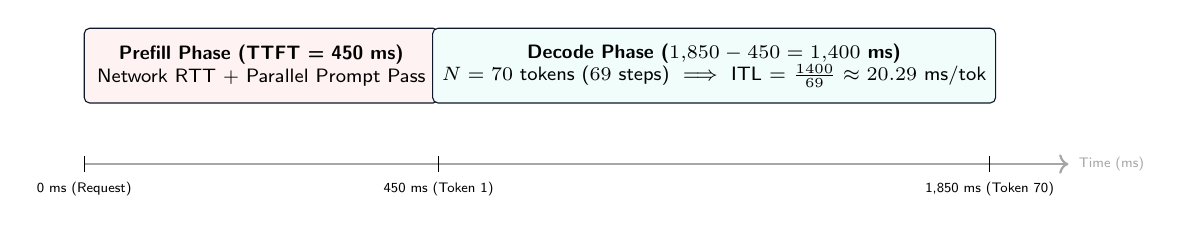
\begin{tikzpicture}[
  bar/.style={draw=headingblue, fill=codebg, rounded corners=2pt, font=\sffamily\scriptsize, align=center, minimum height=0.95cm}
]

\draw[->, thick, color=gray!70] (0,0) -- (12.5,0) node[right, font=\tiny\sffamily] {Time (ms)};
\draw[shift={(0,0)}] (0pt,3pt) -- (0pt,-3pt) node[below, font=\tiny\sffamily] {0 ms (Request)};
\draw[shift={(4.5,0)}] (0pt,3pt) -- (0pt,-3pt) node[below, font=\tiny\sffamily] {450 ms (Token 1)};
\draw[shift={(11.5,0)}] (0pt,3pt) -- (0pt,-3pt) node[below, font=\tiny\sffamily] {1,850 ms (Token 70)};

\node[bar, fill=warningBg, minimum width=4.5cm] at (2.25, 1.25) {
  \textbf{Prefill Phase (TTFT = 450 ms)}\\
  Network RTT + Parallel Prompt Pass
};

\node[bar, fill=intuitionBg, minimum width=7.0cm] at (8.0, 1.25) {
  \textbf{Decode Phase ($1{,}850 - 450 = 1{,}400\text{ ms}$)}\\
  $N = 70$ tokens ($69$ steps) $\implies$ ITL $= \frac{1400}{69} \approx 20.29\text{ ms/tok}$
};

\end{tikzpicture}
\caption{Streaming Latency Decomposition: Token 1 completes at TTFT (450 ms); the remaining $N - 1 = 69$ intervals govern average Inter-Token Latency (ITL).}
\label{fig:v2-ch07-ttft}
\end{figure}

Notice why we divide by $N_{\text{completion}} - 1$ when computing average \textbf{Inter-Token Latency (ITL)}: Token 1 arrives at TTFT, leaving $N - 1$ inter-token intervals across $(t_{\text{end}} - \text{TTFT})$:
\begin{equation}
\text{ITL} = \frac{t_{\text{completion}} - \text{TTFT}}{N_{\text{completion}} - 1}
\end{equation}
Listing~\ref{lst:v2-ch07-stream} tracks TTFT and per-token ITLs on any streaming generator.

\begin{lstlisting}[language=Python, label={lst:v2-ch07-stream}, caption={Streaming TTFT and ITL Latency Profiler}]
import time

class StreamingMetricsCollector:
    def __init__(self):
        self.start_time: float = 0.0
        self.first_token_time: float = 0.0
        self.end_time: float = 0.0
        self.token_timestamps: list[float] = []

    def start(self) -> None:
        self.start_time = time.perf_counter()

    def record_chunk(self) -> None:
        now = time.perf_counter()
        if not self.token_timestamps:
            self.first_token_time = now
        self.token_timestamps.append(now)

    def finalize(self) -> dict[str, float | int]:
        self.end_time = time.perf_counter()
        total_tokens = len(self.token_timestamps)
        ttft = (self.first_token_time - self.start_time) if total_tokens > 0 else 0.0
        total_duration = self.end_time - self.start_time

        itls = [
            self.token_timestamps[i] - self.token_timestamps[i - 1]
            for i in range(1, total_tokens)
        ]
        avg_itl = (sum(itls) / len(itls)) if itls else 0.0
        p95_itl = sorted(itls)[int(len(itls) * 0.95)] if len(itls) >= 20 else avg_itl

        return {
            "total_duration_sec": total_duration,
            "ttft_sec": ttft,
            "total_completion_tokens": total_tokens,
            "avg_itl_ms": avg_itl * 1000.0,
            "p95_itl_ms": p95_itl * 1000.0,
        }
\end{lstlisting}

\textbf{Step-by-Step Trace:} If \texttt{start()} records $t=0.000$ s and 4 tokens arrive at $0.450, 0.470, 0.495, 0.510$ s: \texttt{ttft = 0.450} s, \texttt{itls = [0.020, 0.025, 0.015]} ($N-1 = 3$ intervals), \texttt{avg\_itl\_ms = 20.0} ms, and \texttt{total\_duration\_sec = 0.510} s.

\section{Token Economics and Multi-Tenant Cost Attribution}

Production AI platforms track spend per tenant and feature using three-tier pricing (uncached input, cached prefix input, and output completion tokens):
\begin{equation}
\text{Cost} = \frac{N_{\text{uncached}}}{10^6} P_{\text{in}} + \frac{N_{\text{cached}}}{10^6} P_{\text{cache}} + \frac{N_{\text{out}}}{10^6} P_{\text{out}}
\end{equation}
Table~\ref{tab:model_pricing} lists reference pricing tiers used in Listing~\ref{lst:v2-ch07-cost} and Exercise~\thechapter.2.

\begin{table}[htbp]
\centering
\small
\begin{tabular}{lccc}
\toprule
\textbf{Model Identifier} & \textbf{Input (\$/1M)} & \textbf{Cached Input (\$/1M)} & \textbf{Output (\$/1M)} \\
\midrule
\texttt{gpt-4o} & \$2.50 & \$1.25 & \$10.00 \\
\texttt{claude-3-5-sonnet-20241022} & \$3.00 & \$0.30 & \$15.00 \\
\texttt{gpt-4o-mini} & \$0.15 & \$0.075 & \$0.60 \\
\bottomrule
\end{tabular}
\caption{Illustrative LLM Token Pricing Tiers (USD per 1 Million Tokens).}
\label{tab:model_pricing}
\end{table}

\begin{lstlisting}[language=Python, label={lst:v2-ch07-cost}, caption={Multi-Tenant Token Cost Ledger}]
from dataclasses import dataclass

@dataclass(frozen=True)
class ModelPricing:
    input_per_million: float
    cached_input_per_million: float
    output_per_million: float

PRICING_TABLE = {
    "gpt-4o": ModelPricing(2.50, 1.25, 10.00),
    "claude-3-5-sonnet-20241022": ModelPricing(3.00, 0.30, 15.00),
    "gpt-4o-mini": ModelPricing(0.15, 0.075, 0.60),
}

class CostLedger:
    def __init__(self):
        self.tenant_spend: dict[str, float] = {}

    def record_usage(
        self, tenant_id: str, model: str,
        prompt_tokens: int, cached_tokens: int, completion_tokens: int
    ) -> float:
        pricing = PRICING_TABLE.get(model, PRICING_TABLE["gpt-4o"])
        uncached_prompt = max(0, prompt_tokens - cached_tokens)
        cost = (
            (uncached_prompt / 1_000_000.0) * pricing.input_per_million
            + (cached_tokens / 1_000_000.0) * pricing.cached_input_per_million
            + (completion_tokens / 1_000_000.0) * pricing.output_per_million
        )
        self.tenant_spend[tenant_id] = self.tenant_spend.get(tenant_id, 0.0) + cost
        return cost
\end{lstlisting}

\section{PII Redaction and Tail-Based Sampling}

Exporting raw prompts to third-party trace platforms risks violating GDPR, HIPAA, or PCI-DSS if users paste SSNs, card numbers, or API keys. Scrub attributes in-process before spans leave the service (Figure~\ref{fig:v2-ch07-pipeline} and Listing~\ref{lst:v2-ch07-pii}).

\begin{figure}[htbp]
\centering
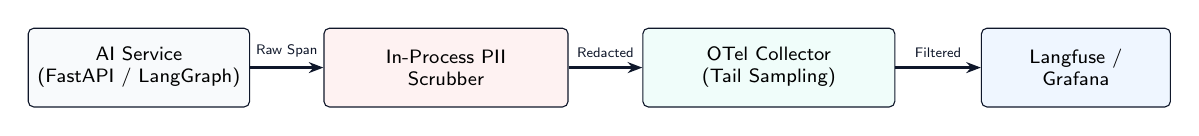
\begin{tikzpicture}[
  box/.style={draw=headingblue, fill=codebg, rounded corners=2pt, font=\sffamily\scriptsize, align=center, minimum height=1.0cm},
  arrow/.style={-{Stealth[scale=0.8]}, thick, color=headingblue}
]

\node[box, minimum width=2.7cm] (app) at (0, 0) {AI Service\\(FastAPI / LangGraph)};
\node[box, fill=warningBg, minimum width=3.1cm] (filter) at (3.9, 0) {In-Process PII\\Scrubber};
\node[box, fill=intuitionBg, minimum width=3.2cm] (collector) at (8.0, 0) {OTel Collector\\(Tail Sampling)};
\node[box, fill=exampleBg, minimum width=2.4cm] (langfuse) at (11.9, 0) {Langfuse /\\Grafana};

\draw[arrow] (app) -- (filter) node[midway, above, font=\tiny\sffamily] {Raw Span};
\draw[arrow] (filter) -- (collector) node[midway, above, font=\tiny\sffamily] {Redacted};
\draw[arrow] (collector) -- (langfuse) node[midway, above, font=\tiny\sffamily] {Filtered};

\end{tikzpicture}
\caption{Production Telemetry Pipeline: Scrub PII inside the service process before tail-based sampling at the OTel Collector.}
\label{fig:v2-ch07-pipeline}
\end{figure}

\begin{lstlisting}[language=Python, label={lst:v2-ch07-pii}, caption={In-Process Regex PII Scrubber}]
import re

class PIIScrubber:
    def __init__(self):
        self.patterns = [
            (re.compile(r"\b\d{3}-\d{2}-\d{4}\b"), "[REDACTED_SSN]"),
            (re.compile(r"\b(?:\d{4}[ -]?){3}\d{4}\b"), "[REDACTED_CARD]"),
            (re.compile(r"(sk-[a-zA-Z0-9]{20,}|ghp_[a-zA-Z0-9]{36})"), "[REDACTED_KEY]"),
        ]

    def scrub(self, text: str) -> str:
        for pattern, replacement in self.patterns:
            text = pattern.sub(replacement, text)
        return text
\end{lstlisting}

\begin{underthehoodbox}[Head-Based vs Tail-Based Sampling]
At 10 million daily requests, storing 100\% of verbose prompt spans is prohibitively expensive. \textbf{Head-based sampling} flips a coin at the start of a request (keeping say 1\%)—meaning 99\% of rare errors and slow outliers vanish! \textbf{Tail-based sampling} buffers spans briefly in the OTel Collector until the trace finishes, keeping 100\% of errors and slow traces ($>5$ s) while retaining only 0.5\% of routine fast traces.
\end{underthehoodbox}

\begin{realworldbox}[Isolating a Cascading SQL Tool Bottleneck via Span Waterfall]
On a routine Tuesday afternoon, an enterprise order-assistant's $p99$ latency climbed from 2.1 s to 58 s. Inspecting a single slow trace waterfall in Langfuse pinpointed the culprit immediately:
\begin{lstlisting}[basicstyle=\ttfamily\scriptsize]
TraceID: 91c8e2... (total=58,140 ms)
  |-- VectorSearch (pgvector)          18 ms
  |-- chat.completion (gpt-4o, TTFT)  350 ms
  |-- ToolExecution (InventoryCheck) 56,910 ms  <-- SQL Seq Scan on 40M rows!
  +-- chat.completion (final synth)   862 ms
\end{lstlisting}
The LLM and vector store were healthy; the \texttt{InventoryCheck} tool was running an unindexed \texttt{WHERE sku = ... AND warehouse\_id = ...} query across 40 million rows. Adding a composite B-tree index restored $p99$ latency to 1.8 s within 10 minutes.
\end{realworldbox}

\begin{tryityourselfbox}[Instrument an Async Streaming Route with OTel \& TTFT]
Extend Listing~\ref{lst:v2-ch07-fastapi} so that a simulated streaming helper yields 5 token chunks spaced 30 ms apart after an initial 120 ms prefill delay, records TTFT and average ITL via \texttt{StreamingMetricsCollector}, sets \texttt{gen\_ai.usage.output\_tokens = 5}, and prints the exported span JSON to stdout. (Complete solution in Section~7.8.)
\end{tryityourselfbox}

\section{Chapter Summary \protect\& Key Takeaways}
\begin{itemize}[leftmargin=18pt]
  \item \textbf{OpenTelemetry Core}: Traces link spans across services via 128-bit \texttt{TraceID}s, W3C \texttt{traceparent} headers, and Python \texttt{contextvars} (explicitly attached when crossing threads).
  \item \textbf{GenAI Conventions}: Standardize on \texttt{gen\_ai.usage.input\_tokens} and \texttt{gen\_ai.usage.output\_tokens}.
  \item \textbf{Prefill vs Decode}: TTFT reflects compute-bound prefill (accelerated by KV-cache prefix reuse); ITL reflects memory-bandwidth-bound decode divided across $N - 1$ token intervals.
  \item \textbf{Cost \& Privacy}: Attribute spend per tenant using three-tier pricing, scrub PII before export, and use tail-based sampling so errors are never dropped.
\end{itemize}

\section{Exercises}

\subsection*{Mechanics}
\textbf{Exercise \thechapter.1}: A streaming LLM request takes 2,400 ms total to emit 80 completion tokens, with Token 1 arriving at 400 ms. Compute: (1) TTFT, (2) average ITL in ms/token, and (3) decode throughput in tokens/second.

\textbf{Exercise \thechapter.2}: A service sends 100,000 daily requests to \texttt{claude-3-5-sonnet-20241022}. Each request has a static 4,000-token system prompt, a 500-token dynamic user query, and 300 completion tokens. Compute daily cost without vs with prompt caching using the rates in Table~\ref{tab:model_pricing}.

\subsection*{Debugging}
\textbf{Exercise \thechapter.3}: A team instruments FastAPI with OpenTelemetry, yet \texttt{AgentRun} and \texttt{ToolExecution} show up as completely separate top-level traces with different \texttt{TraceID}s whenever \texttt{ToolExecution} runs in \texttt{loop.run\_in\_executor()}. Diagnose the context failure and provide the fix.

\subsection*{Architecture}
\textbf{Exercise \thechapter.4}: Design a PCI-DSS compliant LLM observability architecture across 50 microservices that scrubs cardholder numbers before network export, tracks per-tenant token spend, retains 100\% of errors, and alerts on daily spend anomalies.

\section{Detailed Solutions}

\subsection*{Solution \thechapter.1}
1. $\text{TTFT} = 400\text{ ms}$. 2. Decode duration $= 2400 - 400 = 2000\text{ ms}$ across $80 - 1 = 79$ intervals, so $\text{ITL} = 2000 / 79 \approx 25.32\text{ ms/token}$. 3. Decode throughput $= 79 / 2.0\text{ s} = 39.5\text{ tokens/sec}$.

\subsection*{Solution \thechapter.2}
From Table~\ref{tab:model_pricing} for \texttt{claude-3-5-sonnet-20241022}: \$3.00/1M input, \$0.30/1M cached input, \$15.00/1M output.
\begin{itemize}
  \item \textbf{Without caching}: Input $= 10^5 \times \frac{4500}{10^6} \times \$3.00 = \$1{,}350.00$; Output $= 10^5 \times \frac{300}{10^6} \times \$15.00 = \$450.00$; Total $= \mathbf{\$1{,}800.00/\text{day}}$.
  \item \textbf{With caching}: Cached prefix $= 10^5 \times \frac{4000}{10^6} \times \$0.30 = \$120.00$; Uncached query $= 10^5 \times \frac{500}{10^6} \times \$3.00 = \$150.00$; Output $= \$450.00$; Total $= \mathbf{\$720.00/\text{day}}$ (60\% savings).
\end{itemize}

\subsection*{Solution \thechapter.3}
OpenTelemetry tracks the active span in an \texttt{asyncio} \texttt{ContextVar}. Worker threads spawned by \texttt{run\_in\_executor()} do not automatically inherit the coroutine's \texttt{ContextVar}, so the child span sees no parent and mints a fresh \texttt{TraceID}. Fix: capture \texttt{ctx = otel\_context.get\_current()} on the event-loop side, pass \texttt{ctx} into the executor function, and wrap the body in \texttt{token = otel\_context.attach(ctx)} / \texttt{otel\_context.detach(token)}.

\subsection*{Solution \thechapter.4}
1. \textbf{In-Process Scrubbing}: Run \texttt{PIIScrubber} inside every microservice before span attributes are serialized. 2. \textbf{Internal Collector Gateway}: Export spans over mTLS gRPC to an internal VPC OTel Collector cluster. 3. \textbf{Tail-Based Sampling}: Retain 100\% of errors and $>5$ s traces, 0.5\% of normal traces, while extracting exact \texttt{gen\_ai.usage.*} metrics into Prometheus/ClickHouse for 100\% accurate tenant billing and anomaly alerts.

\subsection*{Solution (Try It Yourself)}
\begin{lstlisting}[language=Python]
async def stream_with_telemetry():
    collector = StreamingMetricsCollector()
    with tracer.start_as_current_span("chat.completion") as span:
        span.set_attribute("gen_ai.request.model", "gpt-4o")
        collector.start()
        await asyncio.sleep(0.12)  # Simulated prefill
        for idx in range(5):
            collector.record_chunk()
            if idx == 0:
                span.add_event("first_token")
            await asyncio.sleep(0.03)  # Simulated decode step
        metrics = collector.finalize()
        span.set_attribute("gen_ai.usage.output_tokens", metrics["total_completion_tokens"])
        span.set_attribute("llm.ttft_ms", round(metrics["ttft_sec"] * 1000, 2))
        span.set_attribute("llm.avg_itl_ms", round(metrics["avg_itl_ms"], 2))
    provider.force_flush()
\end{lstlisting}

\begin{labbridgebox}[Project Bridge]
Combine evaluation and telemetry by inspecting how \texttt{projects/p07-llm-eval-pipeline/evaluator/harness.py} aggregates per-case latency and scores, and consider where OpenTelemetry spans attach around graph nodes in \texttt{projects/p05-langgraph-agent-state/agent/graph.py}.
\end{labbridgebox}

\section{Further Reading \protect\& Citations}
\begin{itemize}[leftmargin=18pt]
  \item OpenTelemetry. (2025). \emph{Semantic Conventions for Generative AI Systems}. \url{https://opentelemetry.io/docs/specs/semconv/gen-ai/}.
  \item W3C. (2021). \emph{Trace Context Recommendation (\texttt{traceparent})}. \url{https://www.w3.org/TR/trace-context/}.
  \item Langfuse. (2025). \emph{Open Source LLM Engineering Platform Documentation}. \url{https://langfuse.com/docs}.
\end{itemize}


\end{document}
